\documentclass[12pt,oneside]{uhthesis}
\usepackage{subfigure}
\usepackage[ruled,lined,linesnumbered,titlenumbered,algochapter,spanish,onelanguage]{algorithm2e}
\usepackage{amsmath}
\usepackage{amssymb}
\usepackage{amsbsy}
\usepackage{caption,booktabs}
\captionsetup{ justification = centering }
%\usepackage{mathpazo}
\usepackage{float}
\setlength{\marginparwidth}{2cm}
\usepackage{todonotes}
\usepackage{listings}
\usepackage{xcolor}
\usepackage{multicol}
\usepackage{graphicx}
\usepackage{array}
\usepackage{makecell}
\floatstyle{plaintop}
\restylefloat{table}
\addbibresource{Bibliography.bib}
% \setlength{\parskip}{\baselineskip}%
\renewcommand{\tablename}{Tabla}
\renewcommand{\listalgorithmcfname}{Índice de Algoritmos}
%\dontprintsemicolon
\SetAlgoNoEnd

\definecolor{codegreen}{rgb}{0,0.6,0}
\definecolor{codegray}{rgb}{0.5,0.5,0.5}
\definecolor{codepurple}{rgb}{0.58,0,0.82}
\definecolor{backcolour}{rgb}{0.95,0.95,0.92}

\lstdefinestyle{mystyle}{
    backgroundcolor=\color{backcolour},   
    commentstyle=\color{codegreen},
    keywordstyle=\color{purple},
    numberstyle=\tiny\color{codegray},
    stringstyle=\color{codepurple},
    basicstyle=\ttfamily\footnotesize,
    breakatwhitespace=false,         
    breaklines=true,                 
    captionpos=b,                    
    keepspaces=true,                 
    numbers=left,                    
    numbersep=5pt,                  
    showspaces=false,                
    showstringspaces=false,
    showtabs=false,                  
    tabsize=4
}

\lstset{style=mystyle}

\title{Sistema de gestión para el funcionamiento de un departamento docente en la facultad de Matemática y Computación de la UH}
\author{\\\vspace{0.25cm}Juan Carlos Casteleiro Wong}
\advisor{\\\vspace{0.25cm}Msc. Fernando Rodriguez Flores\\\vspace{0.2cm}Lic. Alain Cartaya Salabarría}
\degree{Licenciado en Ciencia de la Computación}
\faculty{Facultad de Matemática y Computación}
\date{Fecha\\\vspace{0.25cm}\href{https://github.com/username/repo}{github.com/username/repo}}
\logo{Graphics/uhlogo}
\makenomenclature

\renewcommand{\vec}[1]{\boldsymbol{#1}}
\newcommand{\diff}[1]{\ensuremath{\mathrm{d}#1}}
\newcommand{\me}[1]{\mathrm{e}^{#1}}
\newcommand{\pf}{\mathfrak{p}}
\newcommand{\qf}{\mathfrak{q}}
%\newcommand{\kf}{\mathfrak{k}}
\newcommand{\kt}{\mathtt{k}}
\newcommand{\mf}{\mathfrak{m}}
\newcommand{\hf}{\mathfrak{h}}
\newcommand{\fac}{\mathrm{fac}}
\newcommand{\maxx}[1]{\max\left\{ #1 \right\} }
\newcommand{\minn}[1]{\min\left\{ #1 \right\} }
\newcommand{\lldpcf}{1.25}
\newcommand{\nnorm}[1]{\left\lvert #1 \right\rvert }
\renewcommand{\lstlistingname}{Ejemplo de código}
\renewcommand{\lstlistlistingname}{Ejemplos de código}

\begin{document}



\frontmatter
\maketitle

\begin{dedication}
    A Delfín, el abuelo que me regaló la vida, \\  
    espero no olvidar ninguna 
    de tus enseñanzas.
\end{dedication}
\begin{acknowledgements}
    Agradecimientos
\end{acknowledgements}
\begin{opinion}
 En este trabajo se propone un sistema para la informatización de la gestión de varios procesos académicos de la facultad de Matemática y Computación de la Universidad de La Habana.  El uso de este sistema permitiría evitar errores y ahorrar tiempo.  Además, sienta las bases para poder incorporarles algoritmos de optimización que permitan hacer el proceso aún más cómodo.

 Para realizar esta tesis, Juan Carlos tuvo que estudiar contenidos que no forman parte de su plan de estudio, comprender el funcionamiento de los procesos que refleja en su tesis y actuar creativamente para resolver los problemas que aparecieron durante el proceso. Durante este tiempo de trabajo, Juan Carlos se ha caracterizado por su sobriedad, seriedad y responsabilidad.

 Por todo lo anterior, considero que estamos en presencia de un trabajo excelente, desarrollado por una persona que ha demostrado estar capacitada para desempeñarse como un excelente científico de la computación.

  \vspace{1cm}


  \begin{flushright}
    \underline{\hspace{6.5cm}}\\
    MSc. Fernando Raul Rodriguez Flores

    Facultad de Matemática y Computación
  
    Universidad de la Habana

    Noviembre, 2022
  \end{flushright}

  \begin{flushright}
   \underline{\hspace{6.5cm}}\\
   Lic. Alain Cartaya Salabarría

   Facultad de Matemática y Computación
  
   Universidad de la Habana

   Noviembre, 2022
 \end{flushright}
\end{opinion}
\begin{resumen}
	En la facultad de Matemática y Computación de la Universidad de La Habana es necesario realizar un conjunto de
    procesos para administrar y planificar las actividades docentes. La mayoría de estos procesos se llevan a cabo
    de forma manual por los profesores, restándoles tiempo que pudieran destinar a la investigación
    u otras actividades más productivas.

    La asignación de docencia es una tarea que se realiza todos los semestres, y consiste en determinar los profesores  
    que deben impartir cada asignatura del semestre. 
    La planificación de las tesis se realiza cada año, y consiste en conformar los tribunales para todos los
    trabajos de culminación de estudios, y programar la defensa de los mismos.

    En este trabajo se implementa
    un sistema de gestión para informatizar estos dos procesos.
    Para ello, se diseña una base de datos relacional en la que se modelan los elementos que intervienen en 
    la asignación de docencia y la planificación de las tesis. 
    Se desarrolla una aplicación web que permite la posterior integración de la informatización y/o automatización 
    de otras tareas administrativas de la facultad.

    % Se crea una plataforma que facilite que posteriormente se informaticen y/o automaticen el resto de las tareas 
    % administrativas que se realizan en la facultad.



    \paragraph*{}
  \textbf{\emph{Palabras clave---}} sistema de gestión, aplicación web, diseño de base de datos.
\end{resumen}

\begin{abstract}
  Every year, a series of processes to manage and plan 
  docent activities are required in the Math and Computing 
  Science school at the University of Havana. 
  Most of these processes are being done manually and by 
  the teachers themselves, consuming time that 
  could be used for research and other more productive 
  activities.
  
  % Most of theses
  % processes are being implemented manually by the teachers,
  % consuming time that could be destined to research.

  Docent assigning is a task performed every semester, and
  consists in determining which teachers will teach which 
  subjects during the upcoming semester.
  The planning of the graduation thesis is performed every 
  year, and it consists in selecting the juries for all 
  the degree papers, and scheduling their presetations.
  
  In this work, a management system is implemented to computerize those two processes.
  For this purpose, a relational data base was designed, in which the elements that intervene in docent assigning and thesis planning are modeled.
  A web application was developed, to enable the integration 
  of future computerization or automation of other 
  management tasks.
  
  
  
  

% Every year, a set of processes to administrate and plan docent activities is required in the Math and Computing Science faculty at the University of Havana. Most of theses processes are being implemented manually by the teachers, consuming time that could be destined to research.

% Docent assigning is a task performed every semester, and consists in determining which teachers will teach which subject during the semester.
% The planning of the graduation thesis is performed every year, and it consists in selecting the juries for all the Graduation papers, and programming their defense.

% In this paper a management system is implemented to automate those 2 processes.
% For this purpose, a relational data base is designed, in which the elements that intervene in docent assigning and thesis planning are modeled.
% A web app was developed to enable the integration of the automation of other administrative tasks within the faculty.



	% In the Faculty of Mathematics and Computer Science of the University of Havana
  %   a set of processes are performed to manage and planning teaching activities.
  %   Most of these processes are carried out
  %   manually by the professors, causing them to waste time that they could dedicate to investigation.

  %   Teaching assignment is a task that has to be done every semester, and consists in determinate the professors
  %   who must teach each subject of the semester.
  %   Thesis planning process has to be done every year, and consists in design the tribunals for all
  %   the degree works, and schedule their defenses.

  %   In this work we developed a management system to computerize these two processes.
  %   For this, we designed a relational database for modelate the elements that intervene in
  %   teaching assignment and thesis planning. We developed a web application that allows the later integration 
  %   of computerization and/or automation of other administrative tasks of the faculty.

    \paragraph*{}
  \textbf{\emph{Keywords---}} management system, web application, database design.
\end{abstract}
\tableofcontents
\listoffigures
% \listoftables
% \listofalgorithms
\lstlistoflistings

\mainmatter

\chapter*{Introducción}\label{chapter:introduction}
\addcontentsline{toc}{chapter}{Introducción}

\chapter{Preliminares}\label{chapter:preliminaries}
En este capítulo se presenta una breve introducción a los distintos 
procesos que se llevan a cabo en un departamento de la Facultad
de Matemática y Computación de La Universidad de La Habana, así
como una descripción de las herramientas utilizadas en la 
solución brindada. 

\section{Funcionamiento de la facultad}\label{section:funcionamiento de la facultad}
Cada año en la Facultad de Matemática y Computación de La 
Universidad de La Habana se realizan un conjunto de procesos de 
planificación y administración relacionados con los cursos escolares.
La ejecución de los procesos se lleva a cabo en los distintos
departamentos de la facultad y en su mayoría, si no en su totalidad,
se realizan actualmente de manera manual y no informatizada.
A continuación se describen algunos de estos procesos.

\paragraph{Asignación de docencia:}
Consiste en dadas las asignaturas a impartir en el semestre actual,
realizar una distribución de los profesores del departamento, tal que se 
cumplan ciertas restricciones. Por ejemplo, es necesario impartir
cierta cantidad de horas de conferencia, clases prácticas u otro tipo de actividad 
relacionada con cada asignatura, de acuerdo al plan de estudio al que pertenezca.

\paragraph{Planificación de las evaluaciones en el semestre:}
Por cada asignatura que se imparte en el semestre es necesario realizar un planificación de 
las evaluaciones del curso. Por ejemplo, se deben definir la cantidad de evaluaciones, el tipo 
de evaluación: trabajos de control (TC), intrasemestral, preguntas escritas, proyectos, seminarios, entre 
otros y las fechas en las que se efectuarán estas evaluaciones.

\paragraph{Planificación de los exámenes finales y las revalorizaciones:}
Por cada asignatura es necesario realizar la planificación de los exámenes
finales y revalorizaciones. Este es un proceso complejo, se debe tener en cuenta 
varios factores como la cantidad de locales, con sus respectivas capacidades,
todas las asignaturas no tiene las mismas características, por ejemplo la asignatura de 
Programación requiere de dos días completos consecutivos en el laboratorio para 
la realización de sus exámenes. En el caso de las revalorizaciones
se debe tener en cuenta las asignaturas que tengan estudiantes comunes para no programar los 
exámenes en los mismos horarios. Además se pueden valorar otros factores como el orden en el que 
se programen los exámenes, el nivel de complejidad de las asignaturas.

\paragraph{Confección de los tribunales de tesis:}
Como parte del proceso de graduación cada año 
es necesaria la planificación de los tribunales de tesis para 
realizar las defensas de los trabajos de grado. Para la organización 
de esta tarea se necesita la coordinación de los profesores que formarán parte 
de los tribunales de acuerdo a los horarios asignados, además estos profesores 
deben tener conocimientos sobre los temas que se aborden en las tesis en que participen. \\


Este trabajo se centra en los procesos de asignación de docencia y confección de tribunales
de tesis pero tiene como objetivo el desarrollo de una herramienta informática que permita
la integración del resto de los procesos que ocurren en un departamento de la 
Facultad de Matemática y Computación de La Universidad de La Habana.


% A continuación se describen los procesos de asignación de docencia y 
% confección de tribunales de tesis que son llevados
% a cabo en la Facultad de Matemática y Computación de La 
% Universidad de La Habana:

\subsection{Asignación de docencia}
El proceso de asignación de docencia en un departamento consiste en, 
dadas las asignaturas que se imparten en un semestre y el conjunto de 
profesores del departamento, realizar una distribución que satisfaga los
requerimientos de dichas asignaturas.

% contemplando la experiencia y 
% las preferencias de los profesores.

Las carreras universitarias que se estudian en La Universidad de La Habana están
asociadas a un plan de estudio. El plan de estudio es un programa estructurado
donde se definen los contenidos que forman parte del currículo de los 
graduados. En el plan de estudio de una carrera 
se debe caracterizar la profesión, describir las principales funciones de un profesional y 
los valores a desarrollar durante la carrera. Se realiza una planificación de las distintas 
disciplinas que se deben estudiar. Las disciplinas están compuestas por una o varias 
asignaturas y en el plan de estudio se debe especificar la cantidad de horas clase de 
cada asignaturas, así como el año y semestre en el que se deben impartir.

Cada cierto tiempo el plan de estudio de una carrera universitaria cambia, principalmente
para mantener la formación de los profesionales actualizada con el desarrollo de la 
sociedad. Actualmente en la carrera de Ciencia de la 
Computación de la Facultad de Matemática 
y Computación de La Universidad de La Habana, exiten tres planes de estudios 
vigentes. En el año 2018 se actualizó el plan de estudio para los profesionales de la 
carrera de Ciencia de la Computación, se creó el plan de estudio E, donde el total de años 
de estudio de la carrera se redujo de 5 a 4. Los estudiantes que ingresaron en la facultad en 
el curso 2017-2018 se encuentran en el quinto año de la carrera y se rigen por el plan D. 
Además, en consecuencia a la situación epidemiológica que provocó la epidemia de COVID-19 
fue necesaria la modificación del plan E para la reducción de asignaturas del currículo, creándose 
el plan de estudio E (COVID).   

Las asignaturas que se imparten en una carrera universitaria se distribuyen 
en los departamentos de la facultad, en ocasiones una facultad brinda servicio a otras facultades
para .  
Cada asignatura tiene un total de horas que se deben impartir de acuerdo 
al plan de estudio al que pertenezcan. La distribución del total de horas 
en las distintos tipos de clases como conferencias, clases prácticas, seminarios, 
laboratorios u otros, se maneja por el colectivo de profesores de la asignatura e incluso
puede cambiar de un año a otro. Por ejemplo para la asignatura Modelos de Optimización I, perteneciente
al plan de estudio D, para la carrera de Ciencia de la Computación que 
se imparte en el tercer año, se tiene un total de horas a impartir de 64,
de esas, 32 horas son de conferencia y 32 horas son de clases prácticas.


Los profesores tiene una categoría docente y un grado científico.



La planificación de la asignación de docencia se lleva a cabo por el jefe del 
departamento. Se debe tener en cuenta la experiencia, preferencias y carga docente 
de los profesores para realizar la asignación. 



% sus particularidades, como la cantidad de horas
% a impartir en conferencias, clases prácticas, seminarios, laboratorios u
% otras modalidades, y la cantidad de grupos de clase que reciben dicha 
% actividad. Estas particularidades varían en dependencia de la matrícula 
% del curso y del plan de estudio al que la asignatura pertezca.


% además se tiene que las conferencias se imparten a un solo grupo mientras
% que las clases prácticas a dos.


\subsection{Tribunales de tesis}

El ejercicio de culminación de estudios de pregrado consiste en la 
realización de un trabajo de diploma o tesis.
La tesis es un trabajo de investigación que realizan
los estudiantes bajo la tutela de uno o varios profesores (tutores y cotutores)
sobre un tema que tribute a alguna de las áreas que abarca la carrera.
El ejercicio se compone de dos partes, la escritura de un documento que recoja
todo el proceso investigativo y posteriormente la exposición o defensa del mismo ante 
un tribunal.

El tribunal de tesis debe estar compuesto por tres profesores que asuman los roles de 
secretario, presidente y oponente. Los profesores que integren el tribunal no pueden 
ser tutores o cotutores de la tesis y deben tener 
dominio acerca de los temas que se aborden en la investigación.

Debo hablar de que ser oponente es una carga mucho mayor.
Debo hablar sobre los principales problemas de realizar esa tarea 
de forma manual.


% Para realizar la confección de un tribunal de tesis
% se necesitan definir tres incógnitas fundamentales: el local,
% la fecha y el tribunal. El tribunal debe estar compuesto por tres
% profesores que asuman los roles de secretario, presidente y 
% oponente. Los profesores que integren el tribunal no pueden ser 
% tutores o cotutores de la tesis en cuestión, y deben tener dominio
% sobre el tema que será presentado.
% Para la elección de la fecha y el local se debe tener en cuenta que la 
% defensa de una tesis dura aproximadamente 45 minutos.

% (No se si agregar algo sobre esto)
% lo mismo que en el proceso anterior, mencionar las desventajas de 
% hacer este proceso no informatizado




\section{Descripción del software}
Para la informatización de estos procesos se implementa 
un sistema de gestión a través de una aplicación web,
utilizando un modelo cliente-servidor.
Para el desarrollo en el lado del servidor se hace uso del framework Django, en particular Django Rest Framework, aprovechando la
versatilidad, seguridad, escalabilidad y mantenibilidad
que el framework ofrece.
Mientras que en el lado del cliente se hace uso
del framework Quasar, que se basa en Vue.js, creando una
single-page application (SPA) o aplicación de página única.
A continuación se profundiza en el modelo 
y herramientas utilizadas.

\subsection{Modelo cliente-servidor}
El modelo cliente-servidor es uno de los más populares en
el mundo de la informática actual, es utilizado para el 
desarrollo de todo tipo de aplicaciones, incluso muchos 
de los protocolos utilizados a diario implementan este modelo,
tales como File Transfer Protocol (FTP), Simple Mail Transfer Protocol
(SMTP) y Hypertext Transfer Protocol (HTTP).

El modelo cliente-servidor puede ser definido como una arquitectura
de software compuesta por los proveedores de un recurso o servicio, 
denominados servidores, y los solicitantes del servicio, denominados
clientes. En este modelo se realiza una comunicación de procesos
que implica el intercambio de datos tanto por parte del cliente 
como del servidor, realizando cada uno funciones diferentes. La comunicación
se realiza frecuentemente a través de una red informática, pero 
tanto el cliente como el servidor pueden residir en un mismo sistema.

Entre las principales ventajas que ofrece este modelo se encuentran:

\begin{itemize}
    \item centralización de los recursos, los accesos y la integridad de los datos son controlados por el servidor de forma que un programa cliente defectuoso o no autorizado no pueda dañar el sistema.
    \item división del procesamiento de la aplicación en varios dispositivos.
    \item permite la escalabilidad del sistema, en cualquier momento se puede mejorar la capacidad de procesamiento aumentando la cantidad de servidores sin que el funcionamiento de la red se vea afectado.
    \item la separación en cliente y servidor permite el uso de tecnologías enfocadas en las labores específicas que realiza cada uno. 
\end{itemize}
 


\subsection{Desarrollo del servidor}
Para la implementación de los servicios que consumen los clientes del 
sistema de gestión se hace uso del framework Django. Django es un framework
web de alto nivel, gratuito y de código abierto que permite el desarrollo rápido de 
sitios web seguros y mantenibles. Entre las principales características
del framework se encuentran:

\begin{itemize}
    \item Django sigue la filosofía
    de diseño DRY (Don't Repeat Yourself), brindando un conjunto de funcionalidades implementadas
    por los desarrolladores para evitar la repetición de código en procesos
    comunes en el desarrollo web.
    \item Django implementa el patrón de diseño Model-View-Template (MVT), que
    consta de tres componentes esenciales Modelo, Vista,
    Plantilla. Estas componentes son responsables de diferentes
    partes del código e incluso pueden utililizarse de forma independiente. Al ser MVT una 
    ``loosely coupled architecture'' o una ``arquitectura
    débilmente acoplada'', permite de manera sencilla la integración de componentes
    desarrolladas en paralelo.
    \item Django está implementado en Python, por lo que cuenta con un 
    extenso conjunto de bibliotecas para resolver distintas tareas. Entre
    las bibliotecas más utilizadas resalta Django REST framework, desarrollada 
    para la creación de interfaces de programación de aplicaciones (APIs).
    \item Django proporciona un Object Relational Mapper (ORM) o mapeador
    relacional de objetos, permitiendo la interacción con la base de datos
    de forma orientada a objetos. Brinda la posibilidad de crear tablas, insertar,
    editar, borrar y extraer datos sin escribir consultas SQL, acelerando el proceso
    de desarrollo web. 
    \item Django sigue también la filosofía de ``Batteries Included'' o ``Baterías Incluidas''
    proporcionando una biblioteca estándar rica y versátil con herramientas para
    crear sistemas complejos sin la necesidad de instalar paquetes separados. Algunas de 
    estas ``baterías'' son ``Django Admin'', ``Django ORM'', ``Authentication'' y
    ``HTTP''.
    \item Django cuenta con extensa documentación, desde la documentación oficial hasta 
    contenido en forma de artículos, tutoriales y cursos en línea.
    \item Django es escalable, utiliza una arquitectura de ``shared-nothing'' o ``nada compartido'',
    que permite agregar hardware en cualquier nivel: servidores de bases de datos,
    servidores de almacenamiento en caché o servidores web (REFERENCIA).

\end{itemize}

 


\subsection{Desarrollo del cliente}
Dentro de las tecnologías de desarrollo web más utilizadas, sin duda, 
JavaScript es una de las más populares en la actualidad. JavaScript es 
un lenguaje de programación ligero, interpretado o compilado ``just-in-time''
o ``justo-a-tiempo'' con funciones de primera clase. Es un lenguaje de programación
basado en prototipos, multiparadigma, de un solo hilo, dinámico, con
soporte para programación orientada a objetos, imperativa y declarativa.
Se usa principalmente del lado del cliente, implementado como parte de un navegador 
web permitiendo mejorar las interfaces de usarios y la creación de
páginas web dinámicas[REFERENCIA WIKI].

La popularidad de JavaScript para el desarrollo web ha impulsado
la creación de distintos frameworks, entre los más 
utilizados se encuentran:

\subparagraph{Angular}
Lanzado en 2010, Google está a cargo de desarrollar y 
mantener Angular. La principal filosofía tras Angular es 
tener todo lo que el desarrollador necesita, es un framework
con muchas características integradas, tales como: validaciones 
de formularios, envíos de solicitudes http, enrutamiento y 
manejo de estados, cuenta además con herramientas adicionales
como: línea de comandos, interfaces para el manejo y 
creación de proyectos. Debido a esto muchos han llamado a Angular
una plataforma, más que un framework. Google y Wix se 
encuentran entre las empresas más populares que utilizan
Angular.

\subparagraph{React}
Lanzado en 2013, Facebook desarrolla y mantiene React.
A diferencia de Angular, React se enfoca en ser lo más minimalista posible,
especializada en el desarrollo de interfaces de usuario, describiéndose
a sí misma como una biblioteca. Cuenta con muchas menos funciones integradas
que Angular por lo que se terminan utilizando muchos paquetes o
dependencias de terceros al desarrollar un proyecto, ya sea para enrutamiento, manejo de estados o
envío de solicitudes http.
Whatsapp, Instagram, Paypal, Glassdoor y BBC son algunas de 
las compañías populares que usan React.

\subparagraph{Vue.js}
Lanzado en 2014, su desarrollo y mantenimiento es llevado a 
cabo por un equipo de colaboradores a nivel mundial, siendo  
Evan Yu, su principal creador, un ex ingeniero de Google.
Se puede decir que Vue se encuentra entre Angular y React en cuanto 
a la cantidad de funciones integradas que ofrece, más que React, pero 
menos que Angular. Sitios web como GitLab y Alibaba están usando Vue. \\

COMPARACION CON POPULARIDAD Y DESARROLLO\\
Graficos y datos sobre estos frameworks?\\


En los últimos años, Vue.js se ha convertido
en un fuerte competidor de Angular y React. El 
crecimiento de Vue.js se relaciona con la simplicidad 
del framework, la disponibilidad de bibliotecas, componentes
y materiales de aprendizaje. A pesar de que Vue.js es 
un framework para construir interfaces de usuario no 
proporciona elementos o componentes de interfaz de usuarios. Es por esto que surgen  
otros frameworks encima de Vue.js como una capa más de abstracción, que 
brindan un conjunto de componentes reutilizables y con estilo. Entre 
las más populares se encuentran: Vuetify, Bootstrap Vue y Quasar.
Este último fue el escogido para el desarrollo del front-end del sistema de gestión. 
  



\subparagraph{Quasar}
Es un framework de código abierto desarrollado para Vue.js,
que permite el desarrollo aplicaciones/sitios web de una sola página (SPA),
aplicaciones/sitios web renderizados del lado del servidor (SSR),
aplicaciones web progresivas (PWA), incluso aplicaciones móviles y de 
escritorio, reutilizando el mismo código fuente. 
Entre los principales beneficios que Quasar ofrece 
se encuentran:

\begin{itemize}
    \item más de 70 componentes web personalizables y de alto rendimiento para cubrir la 
    mayoría de las necesidades de la web.
    \item buenas prácticas integradas tales como: compresión de código, 
    manejo avanzado de caché, mapeo de fuentes y carga diferida. 
    \item Quasar-CLI, una herramienta que genera de forma automática la estructura del 
    proyecto en cuestión.
    \item soporte para varios idiomas, incluyendo 
    compatibilidad para idiomas RLT (right to left), tanto para los componentes de Quasar
    como para el código del desarrollador.  
    \item amplia comunidad y documentación.
    \item ofrece una versión UMD (Definición de módulo unificado) para la migraración
    de proyectos existentes sin necesidad de ningún proceso de compilación.
    \item promueve las buenas prácticas para mantener la seguridad de las aplicaciones
    desarrolladas con Quasar, en la documentación oficial se le dedica un capítulo
    a este tema [REF].

\end{itemize}


% La minificación es el proceso de reducir el peso de los archivos de código
% fuente a través de la eliminación de bytes innecesarios como los 
% saltos de línea, espacios adicionales y comentarios. Es uno de 
% los principales métodos utilizados para reducir los tiempos de carga y
% el uso de ancho de banda en los sitios web  (HTML/CSS/JS minification)





\section{Diseño de bases de datos}
El desarrollo de la informática y la computación ha permitido
el almacenamiento de grandes cantidades de datos en espacios 
físicos limitados. Actualmente los sistemas de bases de datos juegan
un papel fundamental en el desarrollo de todo tipo de sistemas computacionales.

El diseño de base de datos es un proceso fundamental a la hora 
de modelar el conjunto de datos y las operaciones que se deseen
realizar sobre ellos. Un correcto diseño de la base de datos
es esencial para garantizar la consistencia de la información,
eliminar datos redundantes, ejecutar consultas de manera 
eficiente y mejorar el rendimiento de la base de datos [\cite{db_book_cap2}]. 

\subsection{Metodología de diseño de bases de datos}
La complejidad de la información y la cantidad de requisitos que se 
deseen modelar en un sistema computacional hacen que el diseño de una 
base de datos no sea una tarea sencilla. Por tanto es común es común 
descomponer el proceso de diseño en tres etapas fundamentales: diseño conceptual,
diseño lógico y diseño físico. 


\subsubsection{Diseño conceptual}
En esta fase se obtiene como resultado una representación 
abstracta y de alto nivel de la realidad a partir de las 
especificaciones de requisitos de usuario [REF libro]. El diseño
conceptual comienza con la identificación de las necesidades de los 
usuarios, que a menudo se pueden obtener a través de: examinar
la documentación existente como formularios, observando y
analizando el procesamiento de la información en el proceso que 
se desea modelar o mediante entrevistas a los usuarios finales [\cite{db_requirement_analysis}].

El objetivo del diseño conceptual es describir el contenido de 
información de la base de datos, mediante un esquema conceptual de
la base de datos [\cite{db_book_cap3}], que es independiente del SGBD
que se utilice para manipular la base de datos.
Los programadores o diseñadores utilizan modelos conceptuales de datos 
para la construcción de esquemas. El modelo entidad-relación es uno 
de los más utilizados para el diseño conceptual de bases de datos. Fue 
introducido por Peter Chen en 1976 [REF], y está formado por 
un conjunto de conceptos que permiten describir la realidad mediante 
representaciones gráficas y lingüísticas.

La metodología utilizada 
para el desarrollo del modelo conceptual de datos para la modelación 
de los procesos de asignación de docencia y confección de tribunales de 
tesis fue la metodología genérica MER/XX, que se basa en un enfoque
híbrido entre el modelo entidad/relacional extendido y los conceptos de la 
modelación orientada a objetos [\cite{db_book_cap2}]. 

El modelo entidad-relación extendido describe con un alto nivel de abstracción
el significado de los datos, las relaciones entre ellos y las reglas de negocio 
de un sistema de información. Sus dos elementos principales son las entidades y 
las relaciones, además existen extensiones al modelo básico 
como atributos de las entidades o cardinalidades de las relaciones, 
que aportan al modelo una mayor expresividad.



\subsubsection{Diseño lógico}
Es el proceso de transformar el esquema conceptual del dominio de la aplicación
que se obtiene en la fase anterior,
en un esquema para el modelo de datos subyacente a un SGBD particular.
Existen diferentes modelos matemáticos utilizados para el diseño lógico
de las bases de datos, tales como: el modelo de listas invertidas[REF], el modelo 
jerárquico[REF], el modelo de redes[REF] y el modelo relacional[REF]. 

El modelo relacional fue propuesto por Edgar Frank Codd en 1970. Es un 
modelo que se basa en la lógica de predicados y en la teoría 
de conjuntos, donde todos los datos se representan en términos de tuplas, 
agrupados en relaciones.

El modelo relacional fue el primer modelo de base de datos que se describió en términos 
matemáticos formales. A pesar de que existen  
implementaciones del modelo de base de datos relacional como lo definió originalmente 
Codd, no han tenido éxito popular hasta el momento. No obstante al modelo relacional se le 
atribuye un gran valor por su desarrollo teórico, que ha sido fundamento de muchos de los 
sistemas de gestión de bases de datos relacionales que se utilizan hoy en la actualidad, como:
MySQL, Oracle, SQL Server, PostgreSQL y Microsoft Access. 

El resultado de esta fase consiste en una descripción de las estructuras 
de datos utilizadas para almacenar la base de datos[\cite{db_book_cap3}], que se 
ajuste al modelo que utilice el SGBD. Esto quiere decir que,
si el modelo conceptual es expresado como un modelo 
entidad-relación y el modelo lógico utilizado en el SGBD es el modelo 
relacional, entonces las entidades, relaciones y los atributos del modelo entidad-relación
deben representarse como relaciones. 

NOTA: ACLARAR el concepto de relación en el modelo relacional


% El objetivo del diseño de bases de datos lógicas es crear 
% tablas bien estructuradas que reflejen adecuadamente el 
% entorno empresarial de la empresa.

\subsubsection{Diseño físico}
En esta etapa se transforma la estructura obtenida en la etapa del diseño
lógico, con el objetivo de conseguir mayor eficiencia. Es necesario
evaluar los aspectos de implementación física relacionados al SGBD que se utilice.
Por ejemplo: si se trabaja con una base de datos relacional, la 
transformación de la estructura puede consistir en crear una nueva relación que 
sea la combinación de varias relaciones o separar una relación en varias relaciones o 
añadir algún atributo calculable a una relación. \\




% Para el almacenamiento de los datos hizo uso de SQLite 3
% como sistema de gestión de bases de datos relacionales,
% el cual viene integrada en Django por defecto.

\subsection{Correcto diseño de bases de datos relacionales}

El diseño de una base de datos mediante el enfoque relacional, es una 
tarea no determinista, es posible obtener distintos esquemas relacionales 
como propuestas de la base de datos.
Un diseño incorrecto de una base de datos puede no responder apropiadamente a las exigencias
del proceso que se modela, y puede conllevar a la generación de dificultades o 
errores en el acceso a los datos. Entre los principales errores o dificultades que se pueden generar
se encuentran:

\begin{itemize}
    \item \textbf{Redundancia en los datos}, provoca un aumento innecesario 
    del tamaño de la base de datos, disminuyendo la eficiencia, además puede provocar 
    inconsistencia de los datos que puede conducir a la corrupción de los mismos. 
    \item \textbf{Violación de la integridad de los datos}, el término ``integridad de los datos'' se 
    refiere a la correctitud y completitud de la información en una base de datos. Cuando los datos son 
    modificados con sentencias INSERT, DELETE o UPDATE la integridad de los datos puede comprometerse.
\end{itemize}



Para lograr un correcto diseño de la base de datos se recomienda aplicar un método formal de 
análisis a cada uno de los esquemas obtenidos intuitivamente durante la fase de diseño conceptual, 
que se conoce como proceso de normalización.

\subsubsection{Normalización}
La normalización de una base de datos es un proceso que consiste 
en aplicar una serie de reglas a las relaciones obtenidas 
tras el paso del modelo entidad-relación (diseño conceptual) al modelo 
relacional (diseño lógico), con el objetivo de minimizar la redundancia de datos.
Cada regla se denomina una ``forma normal'', si se cumple la primera regla, se dice que 
la base de datos está en ``primera forma normal'', si se cumplen las tres 
primeras reglas se dice que la base de datos está en ``tercera forma normal''. El proceso de 
normalización se puede caracterizar como la transformación sucesiva de una colección de 
relaciones hacia una forma más restrictiva, de modo que mientrás mas profundo sea el nivel 
de normalización menor será la redundancia que albergue la base de datos [\cite{db_book_cap4}].
A continuación se introducen las definiciones de las reglas formales:

\begin{itemize}
    \item \textbf{Primera Forma Normal (1FN)}: una relación está en 1FN si y solo si, para 
    cada ocurrencia de la relación, toda tupla contiene exactamente un valor del dominio subyacente en
    cada atributo.
    \item \textbf{Segunda Forma Normal (2FN)}: una relación está en 2FN si, además de estar en 
    1FN, todos los atributos que no forman parte de alguna llave candidata constituyen información 
    acerca de la(s) llave(s) completa(s) y no de algún subconjunto de ella(s).
    \item \textbf{Tercera Forma Normal (3FN)}: una relación está en 3FN si, además de estar en 2FN,
    los atributos que no forman parte de alguna llave candidata constituyen información solo acerca
    de la(s) llave(s) y no acerca de otros atributos.
\end{itemize}


Aunque existen otros niveles de normalización como la ``Forma Normal de Boyce-Codd (BCFN)'',
la ``Cuarta Forma Normal(4FN)'' y la ``Quinta Forma Normal (5FN)'',
se considera que una base de datos en 3FN presenta niveles nulos o 
admisibles de redundancia en los datos[\cite{ws_3FN}].





% Para la implementación del sistema de gestión es necesario el almacenamiento
% y procesamiento de los datos que intervienen en los procesos de asignación de 
% docencia y confección de tribunales de tesis. A continuación se brinda una 
% descripción de cómo se modelaron estos procesos.

\chapter{Descripción de las funcionalidades que se desean}\label{chapter:features}
El objetivo de este trabajo es la creación de una herramienta
que permita informatizar dos de los procesos que se realizan en la Facultad de Matemática y
Computación de la Universidad de La Habana (MATCOM): la asignación de docencia y la planificación de las tesis. 

En este capítulo se describen las funcionalidades que se desean incorporar
en el sistema para cada proceso. 
Para ello, se ilustra el flujo de trabajo actual para 
realizar la asignación de docencia y la planificación de las tesis, resaltando 
cómo y cuándo utilizar las funcionalidades deseadas.
La sección \ref{docencia:cap2} está destinada a la asignación de docencia y 
la sección \ref{tesis:cap2} a la planificación de las tesis.



% el uso de las funcionalidades
% se describe el flujo de trabajo actual para realizar estos procesos y 


% En la sección \ref{docencia:cap2} 
% se ilustra el flujo de trabajo actual para realizar la asignación de docencia y cómo se desean utilizar 
% las funcionalidades y en la sección \ref{tesis:cap2}


% En las siguientes secciones se describen las funcionalidades
% que se desean incorporar para cada proceso. En la sección \ref{docencia:cap2}
% las relacionadas (voz pasiva) con la asignación de docencia y en la sección \ref{tesis:cap2}
% las relacionadas(voz pasiva) con la planificación de las tesis.

% Se desea además que la herramienta sea lo sufientemente 
% extensible para que permita, en un futuro, la integración de otros procesos como: 
% planificación de los exámenes finales y revalorizaciones, planificación de los alumnos ayudantes,
% planificación de los cursos optativos, entre otros.

% El objetivo principal de este trabajo es la creación de
% una herramienta que permita la informatización de los procesos de
% asignación de docencia, confección de los tribunales de tesis y planificación de las defensas
% de las tesis, que se llevan a cabo en la Facultad de Matemática y Computación
% de la Universidad de La Habana.
% Se desea además que la herramienta permita la 
% posterior integración de los procesos que se abordan en la 
% sección \ref{section:funcionamiento de la facultad}.



% El objetivo principal de este trabajo es la creación de
% una herramienta que permita la informatización de los procesos
% de administración y planificación que se llevan a cabo en la Facultad de Matemática y Computación
% de La Universidad de La Habana. 
% Se desea implementar un sistema de 
% gestión para realizar los procesos de asignación de docencia y 
% confección de los tribunales de tesis, y que permita 
% la posterior integración de los procesos que se abordan en la 
% sección \ref{section:funcionamiento de la facultad}.












% La primera funcionalidad que se desea es la informatización
% de los datos que intervienen en estos procesos.
% Una vez se tengan los datos se desea realizar la 
% asignación de docencia de un departamento, así como la
% confección de los tribunales de tesis. A continuación 
% se describen estos procesos.


\section{Asignación de docencia}\label{docencia:cap2}
% Se desea implementar un mecanismo que permita realizar la asignación de docencia 
% facilitando el acceso a toda la información que interviene en este proceso. 
% Las principales funcionalidades que se desean:

Como parte del proceso de informatización de la asignación docente, se 
desea incorporar las siguientes funcionalidades al sistema:

% Existen un conjunto de funcionalidades que se desean incorporar para realizar la asignación de 
% docencia, en el sistema que se propone en este trabajo, como:

\begin{itemize}
    \item Conocer las asignaturas que se deben impartir en un período de tiempo dado, por ejemplo enero-julio 2021.
    \item Conocer durante el proceso de asignación, la carga docente que se le ha asignado a cada profesor.
    \item Exportar la asignación de docencia a un documento con un formato preestablecido, que 
    es el que se utiliza actualmente en la facultad.
\end{itemize}

%     \item Realizar la asignación de docencia en un departamento, mostrando solo los datos relevantes 
%      para el mismo. Por ejemplo, cuando se realice la asignación de docencia para el departamento de Matemática Aplicada, solo 
%      se mostrarán las asignaturas y profesores del mismo.
%     \item Realizar filtrados o búsquedas a partir de los datos que intervienen en la asignación 
%           de docencia. Por ejemplo, saber las asignaturas que debe impartir un profesor en un semestre dado.


% A continuación se describen como se desean utilizar las funcionalidades anteriores durante el 
% proceso de asignación de docencia.


El siguiente ejemplo ilustra 
el flujo del proceso de asignación de docencia y cómo se 
desean utilizar las funcionalidades anteriores.
Supongamos que se desea realizar la asignación docente del departamento de 
Matemática Aplicada en el período enero--julio del curso 2022. A continuación 
se muestran las asignaturas que se deben impartir.

\begin{table}[H]
    \centering
    \begin{tabular}{| c | c | c | c | c |}
        \hline
        \thead{Asignatura}   & \thead{Año} & \thead{Facultad} & \thead{Horas} \\ \hline
        Programación y Algoritmos & M1 & MATCOM     & 64 \\
        \hline
        Seminarios de Problemas   & M1 & MATCOM     & 48 \\
        \hline
        Programación y Algoritmos & M2 & MATCOM     & 32 \\
        \hline
        Inferencia Estadística    & M3 & MATCOM     & 80 \\
        \hline
        Matemática Numérica       & M3 & MATCOM     & 48 \\
        \hline
        Optimización Matemática I & M3 & MATCOM     & 64 \\
        \hline
        Estadística               & C3 & MATCOM     & 64 \\
        \hline
        Modelos de Optimización I & C3 & MATCOM     & 64 \\
        \hline
        Estadística               & G2 & GEOGRAFÍA  & 80 \\
        \hline
        Estadística               & S2 & SOCIOLOGÍA & 80 \\
        \hline
    \end{tabular}
    \caption{Asignaturas que debe impartir el departamento de Matemática Aplicada en el período enero--julio 2022.}
    \label{tabla-asignaturas-cap2}
\end{table}

En la tabla \ref{tabla-asignaturas-cap2} se muestra los datos asociados 
a las asignaturas, como el nombre, el año escolar en el que se imparte, la 
facultad a la que pertenece el año escolar y la cantidad de horas totales. 

El primer requerimiento para el sistema, es que la herramienta muestren las asignaturas que se deben impartir por un 
departamento en un período de tiempo dado, por lo tanto, en este caso, se deberían mostrar todas las asignaturas que aparencen 
en la tabla \ref{tabla-asignaturas-cap2}. 

Para simplificar la descripción del proceso, vamos a asumir que las únicas 
asignaturas que se deben impartir son Optimización Matemática I, Modelos de 
Optimización I y Estadística (GEOGRAFÍA).

A partir de las asignaturas que se deben impartir en el semestre, se debe determinar la cantidad
de grupos de conferencias, clases prácticas o cualquier otra actividad de clase,
así como la distribución del total de horas a impartir en cada una de estas actividades. 
Esta tarea se referencia en el documento como ``planificar la carga de las 
asignaturas''.
En la tabla \ref{tabla-carga-asignatura-cap2} se muestra la planificación de la carga 
de las asignaturas que se deben impartir en este ejemplo.
    

% Al comienzo de un período de tiempo, el jefe de departamento debe realizar la planificación de docencia
% del semestre. Se desea que la herramienta muestre las asignaturas que se deben impartir por ese departamento en el período de tiempo dado.
% Por ejemplo en el período enero-julio del curso 2022, el departamento de Matemática Aplicada debe impartir las siguientes asignaturas.


\begin{table}[H]
    \centering
    \begin{tabular}{| c | c | c | c | c | c |}
        \hline
        \thead{Asignatura}  & \thead{Año} & \thead{Facultad} & \thead{Horas} & \thead{Grupos} & \thead{\makecell{Distribución \\ de horas}  } \\ \hline
        Optimización Matemática I  & M3  & MATCOM  &  64   &  1/1  & 32/32  \\ 
        Modelos de Optimización I  & C3  & MATCOM  &  64   &  1/2  & 32/32  \\ 
        Estadística                & G2  & GEOGRAFÍA  &  80   &  1/2  & 48/32  \\ 
        \hline
    \end{tabular}
    \caption{Carga de las asignaturas}
    \label{tabla-carga-asignatura-cap2}
\end{table}

En las columnas de la tabla \ref{tabla-carga-asignatura-cap2} se muestran: 
el nombre de la asignatura, el año escolar en el cual se imparte, la facultad a la que 
pertenece el año escolar, la cantidad total de horas clase, la cantidad de grupos 
de conferencias y de clases prácticas, y la distribución de horas clase en 
conferencias y clases prácticas. 
Por ejemplo, la primera fila de la tabla indica que la asignatura Optimización Matemática I, 
que se imparte a los estudiantes de tercer año de la carrera 
Matemática, tiene un total de 64 horas clase, que se distribuyen en 32 horas de 
conferencias y 32 horas de clases prácticas,
y que solo existe un grupo para las conferencias y para las clases prácticas.


% Una vez que se definan las cargas de las asignaturas, el jefe del departamento
% comienza el proceso de asignación. Se desea que el sistema muestre
% los profesores que están disponibles para 
% cubrir las actividades de clase de las asignaturas (conferencias, clases prácticas).

A partir de esta información, el jefe del departamento comienza el proceso de asignación.
Se desea que el sistema muestre los profesores que están disponibles para 
cubrir la carga de las asignaturas.
En la tabla \ref{tabla-asignación-cap2} se muestra una posible asignación docente 
para este ejemplo.

\begin{table}[H]
    \centering
    \begin{tabular}{ | c | c | c | c |}
      \hline
      \thead{Asignatura} & \thead{Horas} & \thead{Grupos} & \thead{Profesores}\\
      \hline
      Optimización Matemática I &  64  & 1/1 & \makecell{C: Aymeeé Marrero (32) \\ CP: Gemayqzel Bouza(32)} \\
      \hline
      Modelos de Optimización I   &  64   &  1/2 & \makecell{C: Aymeeé Marrero(16) \\ C: Fernando Rodríguez (16) \\ CP: Daniela González(32) \\ CP: Camila Pérez(32)}    \\ 
      \hline
      Estadística                 &  80   &  1/2 &  \makecell{C: Elianys García (48) \\ CP: Ernesto Borrego(32) \\ CP: Elianys García(32)} \\  
      \hline
    \end{tabular}
    \caption{Posible asignación de docencia.}
    \label{tabla-asignación-cap2}
\end{table}

En la primera fila de la tabla \ref{tabla-asignación-cap2}, se indica 
que las 32 horas de conferencia de la asignatura Optimización Matemática I,
se le asignaron a la profesora Aymeeé Marrero y las 32 horas de clases prácticas a la profesora Gemayqzel Bouza.

Cada vez que el jefe de departamento realice una 
asignación, se desea que se actualice la carga docente que tendrá en el semestre el profesor asignado, de forma que se conozca la carga 
de todos los profesores durante el proceso de asignación.
Para la asignación que se muestra en la tabla \ref{tabla-asignación-cap2}, 
el sistema de gestión debe mostrar las siguientes cargas docentes:

\begin{multicols}{2}
    \begin{itemize}
        \item Aymeeé Marrero: 48 horas
        \item Gemayqzel Bouza: 32 horas 
        \item Fernando Rodríguez: 16 horas 
        \item Daniela González: 32 horas 
        \item Camila Pérez: 32 horas
        \item Elianys García: 80 horas
        \item Ernesto Borrego: 32 horas 
    \end{itemize}
\end{multicols}

En este caso se puede apreciar que la carga docente de la profesora 
Elianys García es mayor que la del resto de los profesores, lo cual se 
quisiera evitar con la implementación de esta funcionalidad. 


Por otra parte, se quiere también que el sistema muestre las asignaturas o 
grupos que faltan por cubrir para cumplir con la planificación de la docencia. 
Además, una vez concluida la asignación, se desea poder exportar la información de la docencia a un documento con el 
formato que se utiliza actualmente en la facultad. 


En la próxima sección se describen las funcionalidades que se desean incorporar para el 
proceso de planificación de las tesis.


\section{Planificación de las tesis}\label{tesis:cap2}
El proceso de planificación de las tesis se puede descomponer en dos subprocesos principales: 
la confección de los tribunales y la programación de las defensas.
Para la planificación de las tesis, se desea disponer de las siguientes funcionalidades.



\begin{itemize}
    \item Cada vez que se agregue una tesis en el sistema, crear un tribunal sin definir para la misma.
    \item Conocer, durante el proceso de confección de los tribunales de tesis, la cantidad de tribunales 
    en los que participa cada profesor.
    \item Una vez se confeccione el tribunal de una tesis, crear un horario sin definir para la defensa de la misma.
    \item Una vez estén definidos los horarios, se desea conocer en cuáles, un determinado profesor no está libre (por participaciones en defensas). 
    Con el objetivo de facilitar cambios necesarios en la programación de los actos de defensa.  
    \item Exportar la confección de los tribunales de tesis a un documento con un formato preestablecido.
    \item Exportar la programación de las defensas de tesis a un documento con un formato preestablecido.
\end{itemize}

% A continuación se describen como se desean utilizar las funcionalidades anteriores
% durante el proceso de planificación de tesis.

Para ilustrar las funcionalidades que se desean durante el proceso de 
planificación de las tesis se utilizará un ejemplo.
En la tabla \ref{tabla-tesis-cap2}, se muestran dos tesis.

\begin{table}[H]
    \centering
    \begin{tabular}{ | c | c | c | c |}
      \hline
      \thead{ID} & \thead{Tesis} & \thead{Estudiante} & \thead{Tutores} \\
      \hline 
             1 & \makecell{Simulación y optimización \\ de movimientos de malabares} & Gustavo Despaigne & Fernando Rodríguez  \\
      \hline
             2 & \makecell{Propagación de epidemias \\ mediante modelos basados \\ en metapoblaciones} & Abel Antonio Cruz & \makecell{Angela M. León \\ José A. Mesejo} \\
      \hline
    \end{tabular}
    \caption{Ejemplo de dos tesis}
    \label{tabla-tesis-cap2}
\end{table}

Las columnas de la tabla \ref{tabla-tesis-cap2} muestran: un identificador, el nombre de la tesis, el nombre del autor y 
los nombres de los tutores

El primer paso es la confección de los tribunales para cada tesis. Se debe definir qué
profesor formará parte de cada tribunal y con qué rol. En este ejemplo 
se asume que los tribunales solo se conformarán por un oponente y un presidente.
A continuación se muestran posibles tribunales para las tesis correspondientes a la 
tabla \ref{tabla-tesis-cap2}.


% El encargado de realizar la planificación de las tesis debe confeccionar un tribunal para 
% cada una de ellas. Se desea que el sistema de gestión muestre los profesores de la facultad para 
% la confección de los tribunales. En el curso 2022 los tribunales estarán compuestos por los tutores, 
% un oponente y un presidente, por tanto solo se deben determinar los profesores que asumirán los roles 
% de oponente y presidente. En la figura tal se muestran posibles tribunales para las tesis correspondientes 
% a la tabla \ref{tabla-tesis-cap2}.

\begin{table}[H]
    \centering
    \begin{tabular}{ | c | c | c | c |}
      \hline
      \thead{ID Tesis} & \thead{Tutores} & \thead{Oponente} & \thead{Presidente} \\
      \hline 
             1 & Fernando Rodríguez & Gemayqzel Bouza & Aymeeé Marrero  \\
      \hline
             2 & \makecell{Angela M. León \\ José A. Mesejo} & Damian Valdés & Gemayqzel Bouza  \\
      \hline
    \end{tabular}
    \caption{Posibles tribunales de tesis}
    \label{tabla-tribunal-tesis-cap2}
\end{table}

Con el objetivo de realizar una distribución equitativa de los profesores en los tribunales de tesis, 
se desea que durante el proceso de confección de los tribunales, se pueda conocer la cantidad en los que participa cada profesor.
En la tabla \ref{tabla-carga-profesores-tribunales}
se muestran las participaciones de los profesores en tribunales 
de acuerdo a la tabla \ref{tabla-tribunal-tesis-cap2}

\begin{table}[H]
    \centering
    \begin{tabular}{ | c | c | c |}
      \hline
      \thead{Profesor} & \thead{Oponente} & \thead{Presidente} \\
      \hline 
             Gemayqzel Bouza & 1 & 1  \\
      \hline
             Aymeeé Marrero & 0 & 1 \\
      \hline
            Damian Valdés & 1 & 0 \\
      \hline
    \end{tabular}
    \caption{Cantidad de tribunales de tesis en los que participa cada profesor}
    \label{tabla-carga-profesores-tribunales}
\end{table}


Una vez que se definan los tribunales de tesis, el próximo paso es 
relizar la programación de las defensas. 
Se debe definir la fecha, hora y local en donde se realizará
el acto de defensa de cada tesis. En la tabla \ref{tabla-defensa-tesis-cap2} se muestran posibles 
horarios para las defensas de las 
tesis que se muestran en la tabla \ref{tabla-tesis-cap2}.

\begin{table}[H]
    \centering
    \begin{tabular}{ | c | c | c | c |}
      \hline
      \thead{ID Tesis} & \thead{Fecha} & \thead{Hora} & \thead{Local} \\
      \hline 
             1 & 10/12/2022 & 2:00 PM & Aula Posgrado  \\
      \hline
             2 & 10/12/2022 & 3:30 PM & Salón del Decanato \\
      \hline
    \end{tabular}
    \caption{Posible horarios para las defensas de tesis}
    \label{tabla-defensa-tesis-cap2}
\end{table}

Una vez concluido el proceso de planificación de las tesis, 
se desea poder exportar los datos de los tribunales y la programación de las 
defensas a documentos con un formato 
preestablecido. 

Con el objetivo de evitar que una tesis se quede sin planificar, se desea que cada vez que una tesis se agregue al sistema, se genere automáticamente 
un tribunal sin definir y una programación para el acto de defensa, sin definir la fecha, la hora ni el local.

Además se desea conocer para cada profesor los horarios que tiene ocupado a partir de la programación de las defensas, 
por si es necesario realizar algún cambio en la planificación.


En este capítulo se describieron las funcionalidades que se desean incorporar en el sistema 
como parte de la informatización de los procesos de asignación de docencia y planificación de las tesis. 
En el próximo capítulo se describe como se modeló y diseñó la base de datos para representar 
la información que interviene en estos procesos. 



\chapter{Descripción del diseño de la base de datos}\label{chapter:database}

\section{Modelación de la asignación de docencia}\label{database:asignación-docencia}
En la fase de diseño conceptual se modelaron las entidades fundamentales
que intervienen en el proceso de la asignación de docencia, 
así como las interrelaciones que se establecen entre ellas
y se obtuvo el siguiente
esquema a partir del modelo entidad-relación extendido.

\begin{figure}[H]
    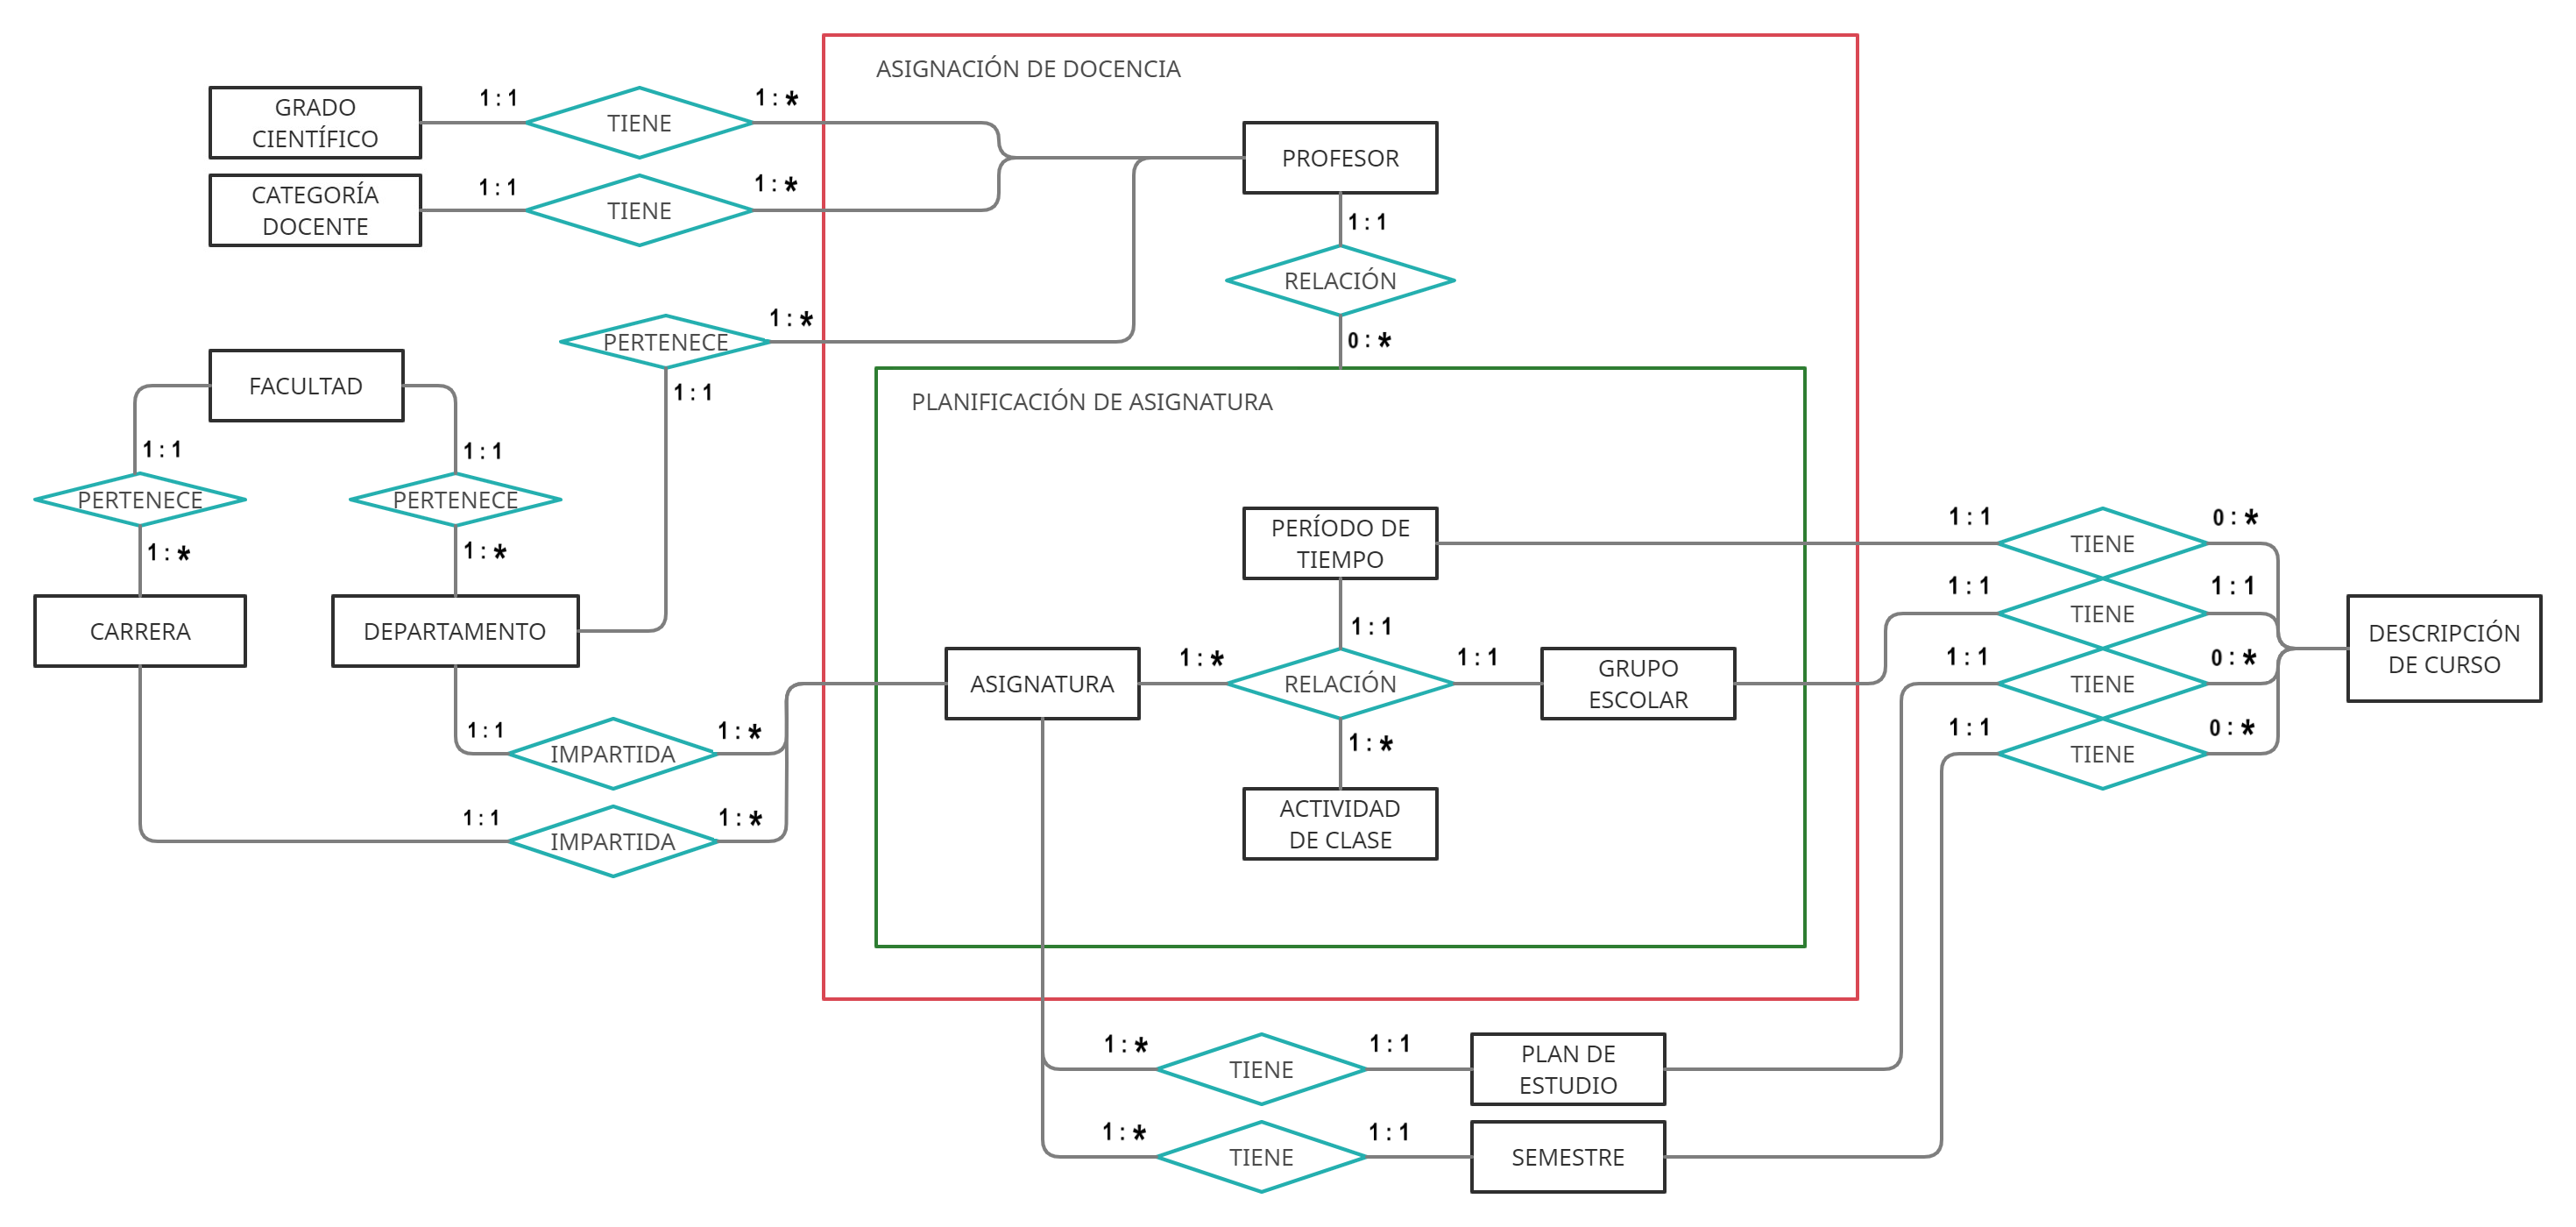
\includegraphics[scale=0.2]{Graphics/Database/MERXX-TA-FINAL.png}
\end{figure}


Con el objetivo de simplificar la representación del modelo entidad-relación
no se agregaron a la imagen los atributos correspondientes a cada entidad, por lo 
que a continuación se describen las entidades en mayor profundidad.


\subparagraph{FACULTAD:}
Representa las facultades de la Universidad de La Habana.
El nombre de la facultad se modela como un atributo, mientras que 
las carreras que se estudian en la facultad y los departamentos que pertenecen 
a ella, se modelan como relaciones con las entidades CARRERA y DEPARTAMENTO, respectivamente.
Una facultad tiene uno o muchos departamentos, y en 
una facultad se pueden estudiar una o más carreras.

\subparagraph{CARRERA:}
Representa las carreras que se estudian en la Universidad de La Habana.
El nombre de la carrera se modela como un atributo, mientras que la facultad a la que pertenece la carrera y
las asignaturas que se imparten en ella, se modelan como relaciones con las entidades FACULTAD y
ASIGNATURA, respectivamente. 
Una carrera pertenece a una única facultad y en una carrera se imparten una o muchas asignaturas.

\subparagraph{DEPARTAMENTO:}
Representa los departamentos de una facultad de la Universidad de La Habana.
El nombre del departamento se modela como un atributo, mientras que los profesores que 
pertenecen a un departamento, las asignatura que son atendidas por el departamento y la 
facultad a la que pertenece el departamento, se modelan como relaciones con las entidades 
PROFESOR, FACULTAD y ASIGNATURA, respectivamente. Un departamento pertenece a una única facultad,
un departamento atiende una o muchas asignaturas y a un departamento pertenecen uno o muchos 
profesores.

\subparagraph{PROFESOR:}
Agrupa los datos asociados a los profesores.
Los campos nombre y apellidos se modelan como atributos,  
mientras que, la categoría docente, el grado 
científico de un profesor y el departamento al que pertenece, se modelan como 
relaciones con las entidades CATEGORÍA DOCENTE, GRADO CIENTÍFICO y 
DEPARTAMENTO, respectivamente. Un profesor pertenece a un único departamento y puede tener solo 
un grado científico y una categoría docente. 


\subparagraph{CATEGORÍA DOCENTE:}
Representa la categoría docente que tienen los profesores.
El nombre de la categoría docente se modela como un atributo. 
Pueden existir uno o muchos profesores con una misma categoría docente.

\subparagraph{GRADO CIENTÍFICO:}
Representa el grado científico que tienen los profesores.
El nombre del grado científico se modela como un atributo.
Pueden existir uno o muchos profesores con un mismo grado científico.





\subparagraph{ASIGNATURA:}
Agrupa los datos asociados a las asignaturas.
Los campos nombre de la asignatura y cantidad de horas 
totales a impartir, se modelan como atributos, mientras que
el plan de estudio asociado a la asignatura, el semestre en el que se 
imparte, el departamento responsable de la asignatura y la carrera a la 
que pertenece, se modelan como relaciones con las entidades
PLAN DE ESTUDIO, SEMESTRE, DEPARTAMENTO y CARRERA respectivamente. Una asignatura 
es atendida por un único departamento, pertenece a una única carrera, se imparte en un 
único semestre y tiene un único plan de estudio. Las asignaturas que se imparten de forma 
anual son representadas como dos asignaturas independientes.

\subparagraph{PLAN DE ESTUDIO:}
Representa el plan de estudio por el que se rige una asignatura.
El nombre del plan de estudio se modela como un atributo.
Pueden existir una o muchas asignaturas con el mismo plan de estudio.



\subparagraph{SEMESTRE:}
Representa los semestres asociados a una carrera. 
El nombre del semestre se modela como un atributo.
Pueden existir una o muchas asignaturas que se imparten en 
el mismo semestre. 

\subparagraph{CURSO ESCOLAR:}
Representa los cursos escolares.
El nombre del curso escolar se modela como un atributo.
Pueden existir una o muchas asignaturas que se imparten en 
el mismo curso escolar.


\subparagraph{PERÍODO DE TIEMPO:}
Representa los períodos de tiempo del año.
El nombre del período de tiempo se modela como un atributo.
Pueden existir una o muchas asignaturas que se imparten en 
el mismo período de tiempo.


\subparagraph{GRUPO ESCOLAR:}
Representa los años académicos asociados a una carrera, como por ejemplo:
Matemática primer año (M1) o Computación tercer año (C3).
El nombre del grupo escolar se modela como un atributo.

\subparagraph{ACTIVIDAD DE CLASE:}
Representa los tipos de actividades que se imparten en una asignatura, 
tales como: conferencias, clases prácticas, seminarios, laboratorios, otros. 

\subparagraph{PLANIFICACIÓN DE ASIGNATURA:}
Se crea con el objetivo de modelar la separación de una asignatura
según las actividades de clases a impartir, en un período de tiempo y para
un grupo escolar específico. Está compuesta por la agregación de las entidades ASIGNATURA, ACTIVIDAD DE CLASE, GRUPO 
ESCOLAR, CURSO ESCOLAR Y PERÍODO DE TIEMPO.
Se agregan los atributos cantidad de horas para el tipo de actividad a realizar y 
la cantidad de grupos.
Por ejemplo (poner ejemplo real de una asignatura
con distintas act de clase y como queda la separación)



% Entidad creada con el objetivo de separar las distintas actividades 
% que se imparten en una asignatura ( conferencia, clases 
% prácticas, seminarios, laboratorios, otras )  para
% realizar la asignación de docencia. Cuenta con una ASIGNATURA,
% en un PERÍODO DE TIEMPO, con el tipo de ACTIVIDAD DE CLASE y 
% el GRUPO ESCOLAR correspondiente. Por ejemplo, una planificación de
% asignatura pudiera ser (Poner ejemplo real). 
% se hace necesaria 
% la separación de una ASIGNATURA en más de una instancia para representar 
% el tipo de actividad de clase ( conferencia, clases 
% prácticas, seminarios, laboratorios, otras ), que va a recibir un 
% grupo escolar, en un período de tiempo.



\subparagraph{ASIGNACIÓN DE DOCENCIA:}
Representa las asignaciones de planificaciones de asignaturas a profesores.
Además se agrega un atributo porciento que indica el porcentaje del total de horas 
a impartir que asume el profesor asignado. Un profesor puede 
tener asignada cero o muchas planificaciones de asignaturas y una planificación de 
asignatura puede estar asignada a uno o muchos profesores.


\subparagraph{DESCRIPCIÓN DE CURSO:}
Representa el grupo escolar vigente en el curso actual. Está 
compuesta por la agregación de las entidades GRUPO ESCOLAR,
PERÍODO DE TIEMPO, PLAN DE ESTUDIO y SEMESTRE.  
Por ejemplo, una DESCRIPCIÓN DE CURSO puede ser 
que el grupo escolar C4 (Computación de cuarto año), con plan de
estudio E, se encuentra en el semestre 8,  en el período de tiempo septiembre-diciembre.






\section{Modelación de los tribunales de tesis}
Para la modelación del proceso de confección de los tribunales de tesis,
se crea un esquema basado en el modelo entidad-relacional extendido como en el 
proceso anterior. 


\begin{figure}[H]
    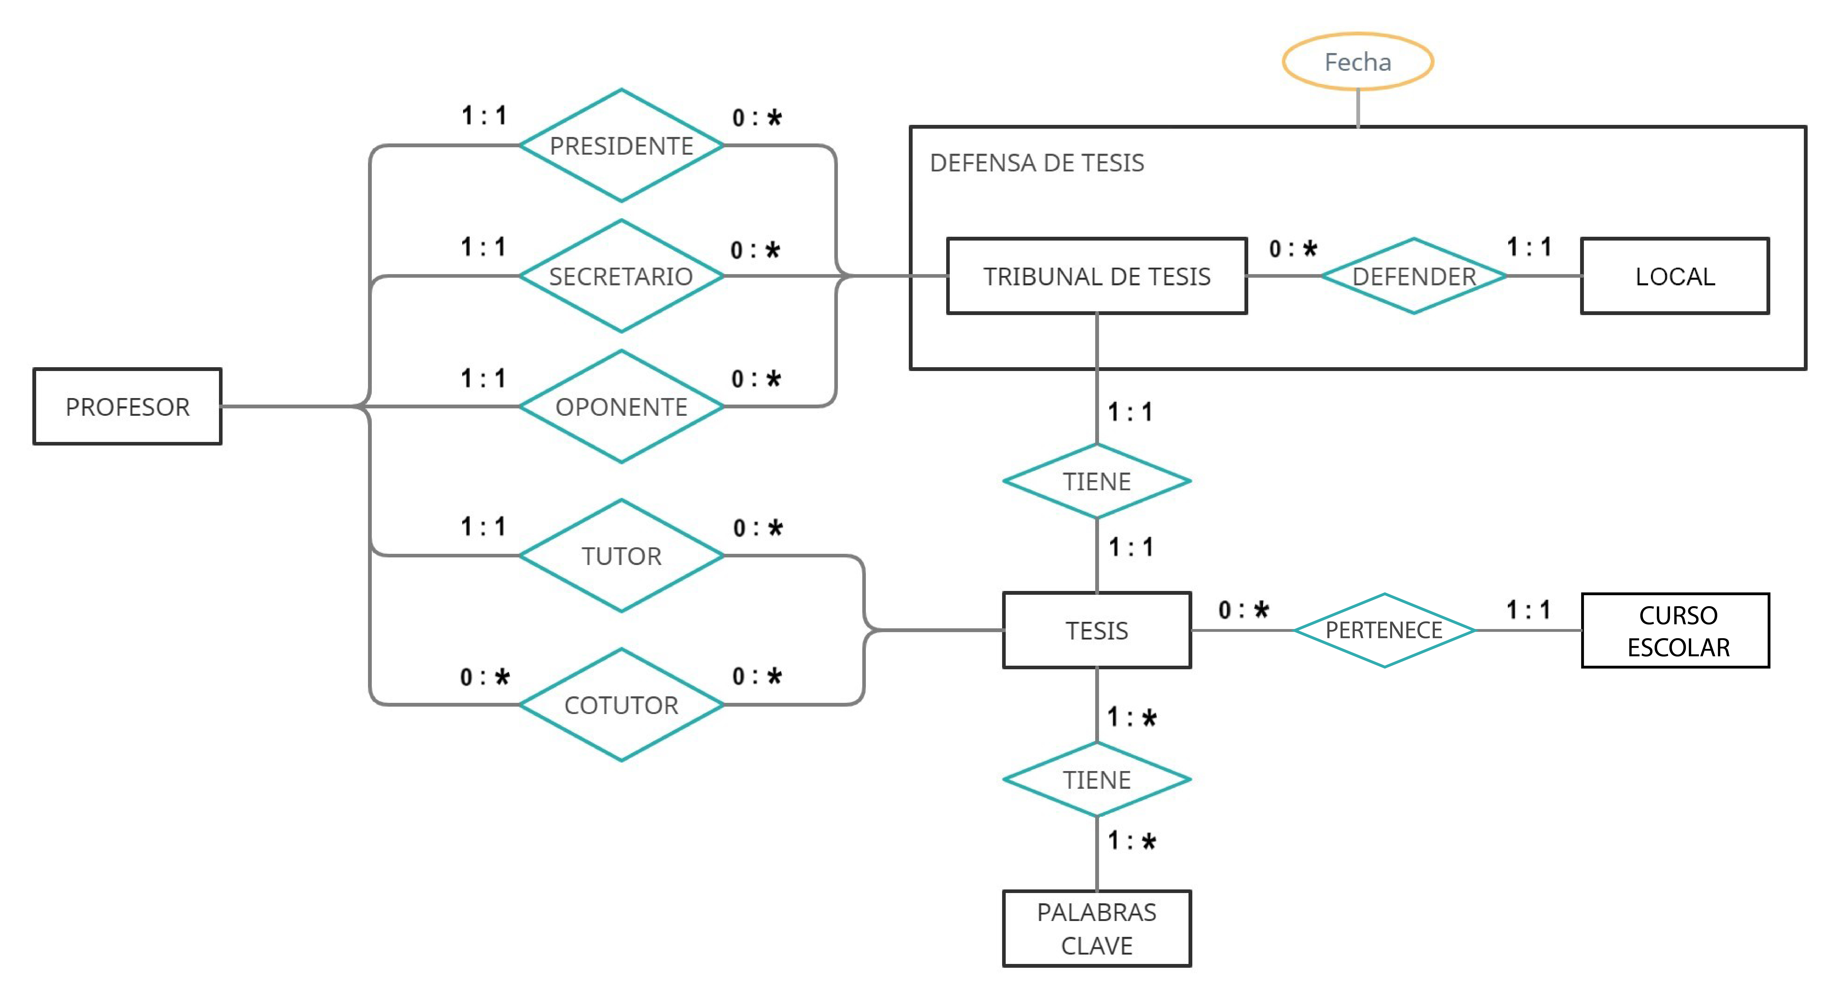
\includegraphics[scale=0.22]{Graphics/Database/MERXX-TC-FINAL.png}
    \caption{}
    \label{mern-ta}
\end{figure}


\subparagraph{TESIS:}
Agrupa los datos asociados a una tesis.
El título de la tesis y el autor se modelan como atributos, mientras que
el tutor, los cotutores, curso escolar y las palabras claves se modelan como relaciones con 
las entidades PROFESOR (tutor y cotutores), CURSO ESCOLAR y PALABRAS CLAVES.
Una tesis tiene un único tutor, puede tener cero o muchos cotutores, pertenece a 
un único curso escolar y tiene una o muchas palabras claves. 

\subparagraph{PALABRAS CLAVES:}
Representa las palabras claves que describen el contenido de una tesis.
El nombre o texto de las palabras claves se modela como un atributo. Una 
palabra clave puede aparecer en una o muchas tesis. 


\subparagraph{TRIBUNAL DE TESIS:}
Representa el tribunal de la defensa de una tesis.
Está compuesto por los miembros del tribunal: presidente, secretario y oponente, 
y la tesis, campos que se modelan como relaciones con las entidades PROFESOR y TESIS, respectivamente.
Un tribunal de tesis tiene una única tesis, un único presidente, un único secretario y 
un único oponente.


\subparagraph{DEFENSA DE TESIS:}
Representa el acto de defensa de la tesis. 
Está compuesta por un tribunal de tesis, en un local y una 
fecha determinada. La fecha se modela como un atributo mientras que 
el tribunal y el local se modelan como relaciones con las entidades TRIBUNAL DE 
TESIS y LOCAL, respectivamente. Una defensa de tesis tiene un único tribunal de tesis,
una única fecha y un único local.



\subparagraph{LOCAL:}
Representa el local donde se lleva a cabo la defensa de las tesis.
El nombre del local se modela como un atributo. 
En un local se puede realizar la defensa de cero o muchas tesis.


\subparagraph{PROFESOR:}
Se utiliza la misma entidad creada en el proceso de asignación de docencia.
Un profesor puede tener el rol de presidente, secretario u oponente en cero o 
muchos tribunales de tesis. Un profesor puede ser 
tutor o cotutor de cero o muchas tesis. \\


DESPUES DE LA MODELACION DE CADA PROCESO CREO Q DEBO HABLAR UN 
POCO DEL PROCESO DE NORMALIZACION PARA ESOS ESQUEMAS, Y REVISAR SI 
ESTAN EN 3FN... 

NO SE QUE MAS MENCIONAR EN ESTE CAPITULO.



\chapter{Descripción las herramientas implementadas}\label{chapter:implementation}
El objetivo de este trabajo es la informatización de los 
procesos de asignación de docencia y 
planificación de las tesis que se llevan a cabo 
en la Facultad de Matemática y Computación de la Universidad de La Habana (MATCOM). 

En este capítulo se presenta la aplicación web que se implementó 
como propuesta de solución para la informatización de estos procesos. 
En las secciones \ref{cap4:docencia} y \ref{cap4:tesis} se describen los pasos que se deben 
seguir para realizar a través del sistema, la asignación de docencia y la planificación de las tesis, respectivamente.
En la sección \ref{cap4:csv} se describe una funcionalidad que se implementó en el lado del servidor 
para salvar el estado de la base datos en documentos CSV y poblar la base de datos a partir de los mismos.

% P

% En este capítulo se presenta 

% la propuesta de solución para 
% la informatización de los procesos de asignación de docencia y 
% planificación de las tesis que se llevan a cabo 
% en la Facultad de Matemática y Computación de la Universidad de La Habana. 




% Se implementó un sistema de gestión siguiendo el modelo cliente-servidor. El desarrollo del servidor se efectuó con el uso Django, en 
% particular Django Rest Framework y el cliente se desarrolló utilizando
% Quasar para la creación de las interfaces de usarios. Para almacenar los datos que 
% se utilizó una base de datos SQLite.

En la figura \ref{img-home-page} se ilustra la vista inicial de la 
aplicación web que se implementó. En la parte superior se encuentra una 
barra de navegación, desde la cual se puede acceder a todas las vistas 
de la aplicación. Se crearon dos paneles principales, uno para la administración de 
los departamentos y otro para la planificación de las tesis. En el 
panel para la administración de los departamentos se muestran los cuatro departamentos 
de la facultad MATCOM, con cuatro botones cada uno que llevan a las vistas 
para administrar los profesores, las asignaturas, las cargas de las asignaturas 
y las asignaciones de docencia correspondientes al departamento.
En el panel para la planificación de las tesis se agregó un selector para definir qué curso escolar 
se desea planificar y tres botones que 
llevan a las vistas para administrar las tesis, los tribunales y las defensas, correspondientes 
al curso escolar seleccionado.

  


\begin{figure}[H]
    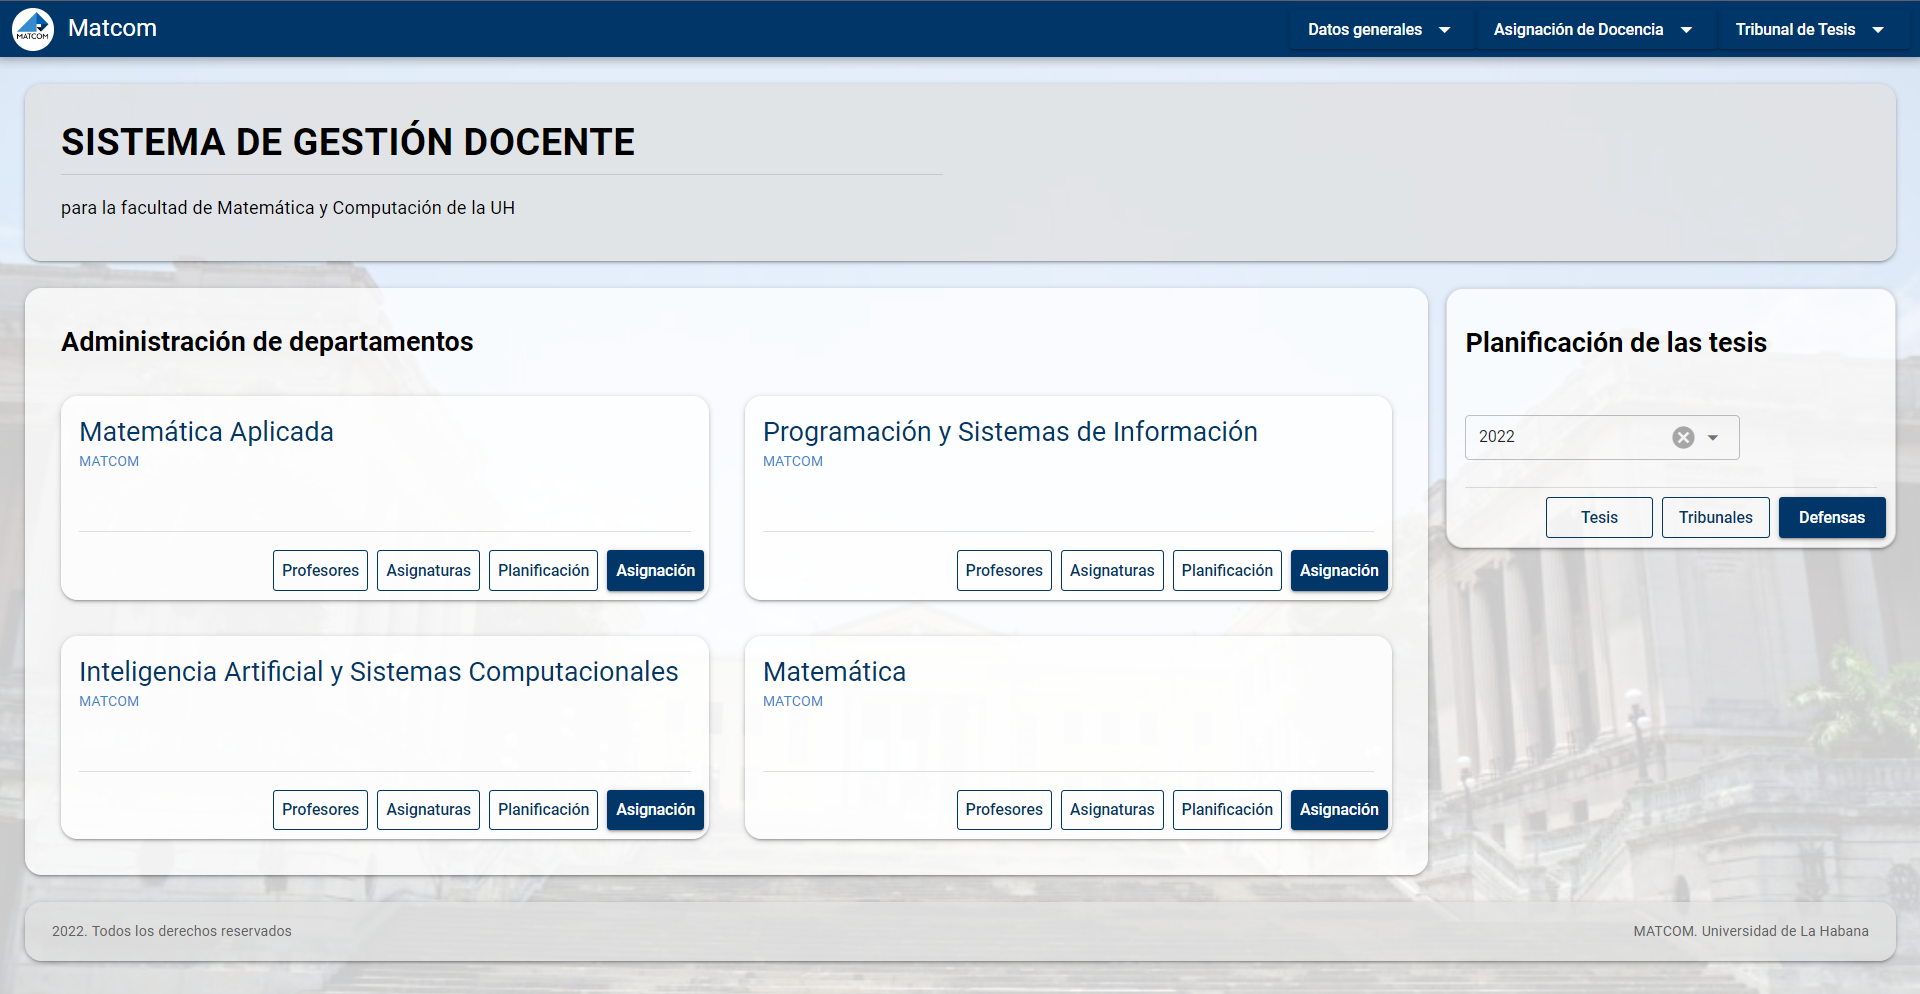
\includegraphics[scale=0.3]{Graphics/Implementation/Home-page.png}
    \caption{Vista inicial del sistema de gestión}
    \label{img-home-page}
\end{figure}






\section{Asignación de docencia}\label{cap4:docencia}

% El proceso de asignación de docencia en un departamento se realiza en la 
% interfaz que se muestra en la figura \ref{img-ta-done}. El usuario de la 
% aplicación puede ver la carga docente de los profesores durante el proceso 
% de asignación, realizar filtrados por profesor para ver las asignaturas 
% que tiene asignada y descargar un documento CSV que contiene la información 
% de la docencia una vez haya terminado la asignación.



En esta sección se describen los pasos que se deben seguir para realizar 
el proceso de asignación de docencia en un departamento a través del sistema 
de gestión que se propone en este trabajo. 
Para la ilustrar este proceso se utilizará 
el mismo fragmento de la docencia correspondiente al departamento
de Matemática Aplicada en el período de tiempo 
enero--julio del curso 2022, que se describe en la sección \ref{docencia:cap2}. 
En la tabla \ref{tabla-carga-asignaturas-cap4} 
se muestra la carga de las asignaturas que se deben impartir
y en la \ref{tabla-carga-asignaturas-cap4} 
la distribución de los profesores
para cubrir con la docencia. 
% Supongamos que se quiere realizar la asignación de docencia para el departamento 
% de Matemática Aplicada   

% \begin{table}[H]
%     \centering
%     \begin{tabular}{| c | c | c | c | c |}
%         \hline
%         \thead{Facultad}   & \thead{Año} & \thead{Asignatura} & \thead{Horas} & \thead{Grupos}  \\ \hline
%         MATCOM     & M3  & Optimización Matemática I  &  64   &  1/1   \\ 
%         MATCOM     & C3  & Modelos de Optimización I  &  64   &  1/2   \\ 
%         GEOGRAFÍA  & G2  & Estadística                &  80   &  1/2   \\ 
%         \hline
%     \end{tabular}
%     \caption{Fragmento de la planificación de docencia.}
%     \label{tabla-planificación-cap4}
% \end{table}

\begin{table}[H]
    \centering
    \begin{tabular}{| c | c | c | c | c | c |}
        \hline
        \thead{Asignatura}  & \thead{Año} & \thead{Facultad} & \thead{Horas} & \thead{Grupos} & \thead{\makecell{Distribución \\ de horas}  } \\ \hline
        Optimización Matemática I  & M3  & MATCOM  &  64   &  1/1  & 32/32  \\ 
        Modelos de Optimización I  & C3  & MATCOM  &  64   &  1/2  & 32/32  \\ 
        Estadística                & G2  & GEOGRAFÍA  &  80   &  1/2  & 48/32  \\ 
        \hline
    \end{tabular}
    \caption{Carga de las asignaturas}
    \label{tabla-carga-asignaturas-cap4}
\end{table}


\begin{table}[H]
    \centering
    \begin{tabular}{ | c | c | c | c |}
      \hline
      \thead{Asignatura} & \thead{Horas} & \thead{Grupos} & \thead{Profesores}\\
      \hline
      Optimización Matemática I &  64  & 1/1 & \makecell{C: Aymeeé Marrero (32) \\ CP: Gemayqzel Bouza(32)} \\
      \hline
      Modelos de Optimización I   &  64   &  1/2 & \makecell{C: Aymeeé Marrero(16) \\ C: Fernando Rodríguez (16) \\ CP: Daniela González(32) \\ CP: Camila Pérez(32)}    \\ 
      \hline
      Estadística                 &  80   &  1/2 &  \makecell{C: Elianys García (48) \\ CP: Ernesto Borrego(32) \\ CP: Elianys García(32)} \\  
      \hline
    \end{tabular}
    \caption{Fragmento de la asignación de docencia.}
    \label{tabla-asignación-cap4}
\end{table}


El primer paso que se debe realizar es planificar la carga de las asignaturas 
que se deben impartir, la interfaz de usuario que se implementó en el sistema para realizar 
este proceso se muestra en la figura \ref{img-pd-example}.

\begin{figure}[H]
    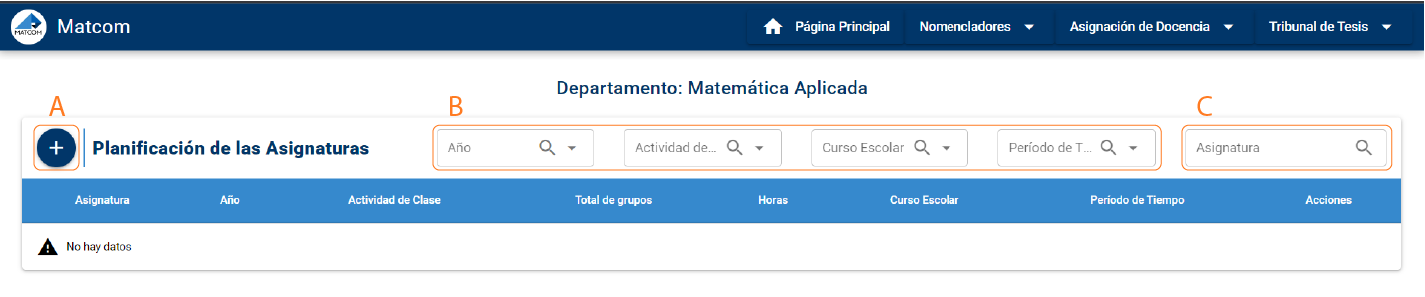
\includegraphics[scale=0.3]{Graphics/Implementation/Docencia/PD-empty.png}
    \caption{Vista de la planificación de las cargas de las asignaturas}
    \label{img-pd-example}
\end{figure}


En la figura \ref{img-pd-example},
se indican con recuadros tres regiones cuyo significado se explica a continuación.

\begin{itemize}
    \item A: botón para agregar una nueva carga de asignatura.
    \item B: filtros por: Año, Actividad de clase, Curso escolar, Período de tiempo.
    \item C: barra de búsqueda por texto para el nombre de las asignaturas. 
\end{itemize}


Para agregar una nueva carga de asignatura se debe pulsar en el 
botón que se indica en el recuadro A y completar los campos del formulario. 
En la figura \ref{img-pd-form} se muestra como agregar la planificación
correspondiente a las conferencias de la asignatura Optimización
Matemática I para los estudiantes de tercer año de la carrera Matemática. 

\begin{figure}[H]
    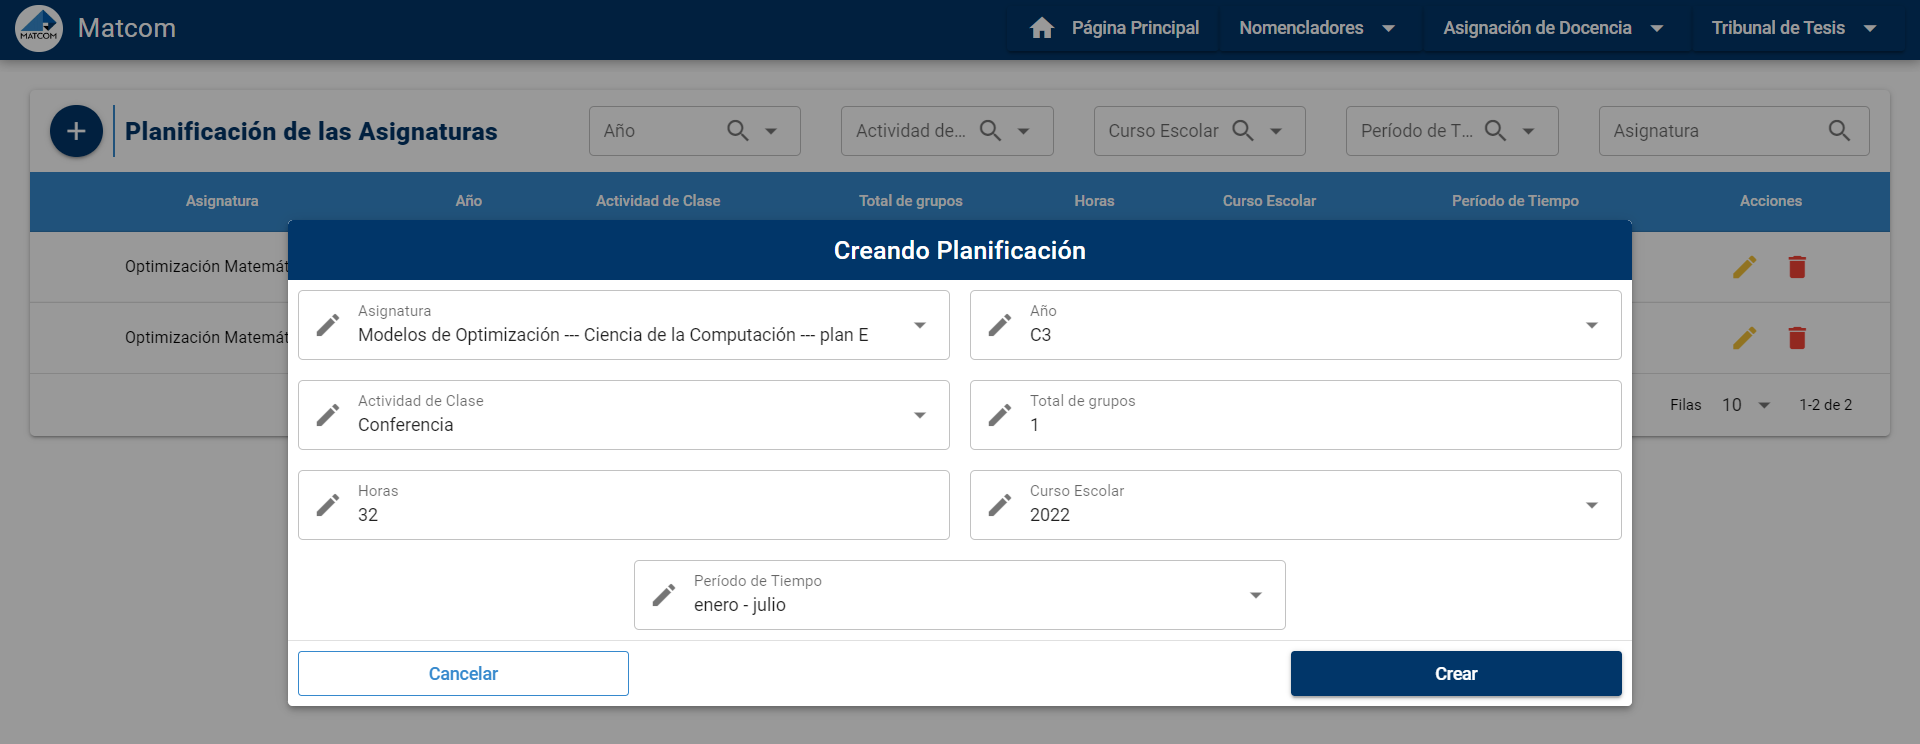
\includegraphics[scale=0.3]{Graphics/Implementation/Docencia/PD-form.png}
    \caption{Vista del formulario para crear una carga de asignaturas}
    \label{img-pd-form}
\end{figure}


La figura \ref{img-pd-result} muestra el resultado de agregar las planificaciones de las asignaturas 
correspondientes a la tabla \ref{tabla-carga-asignaturas-cap4}. 


\begin{figure}[H]
    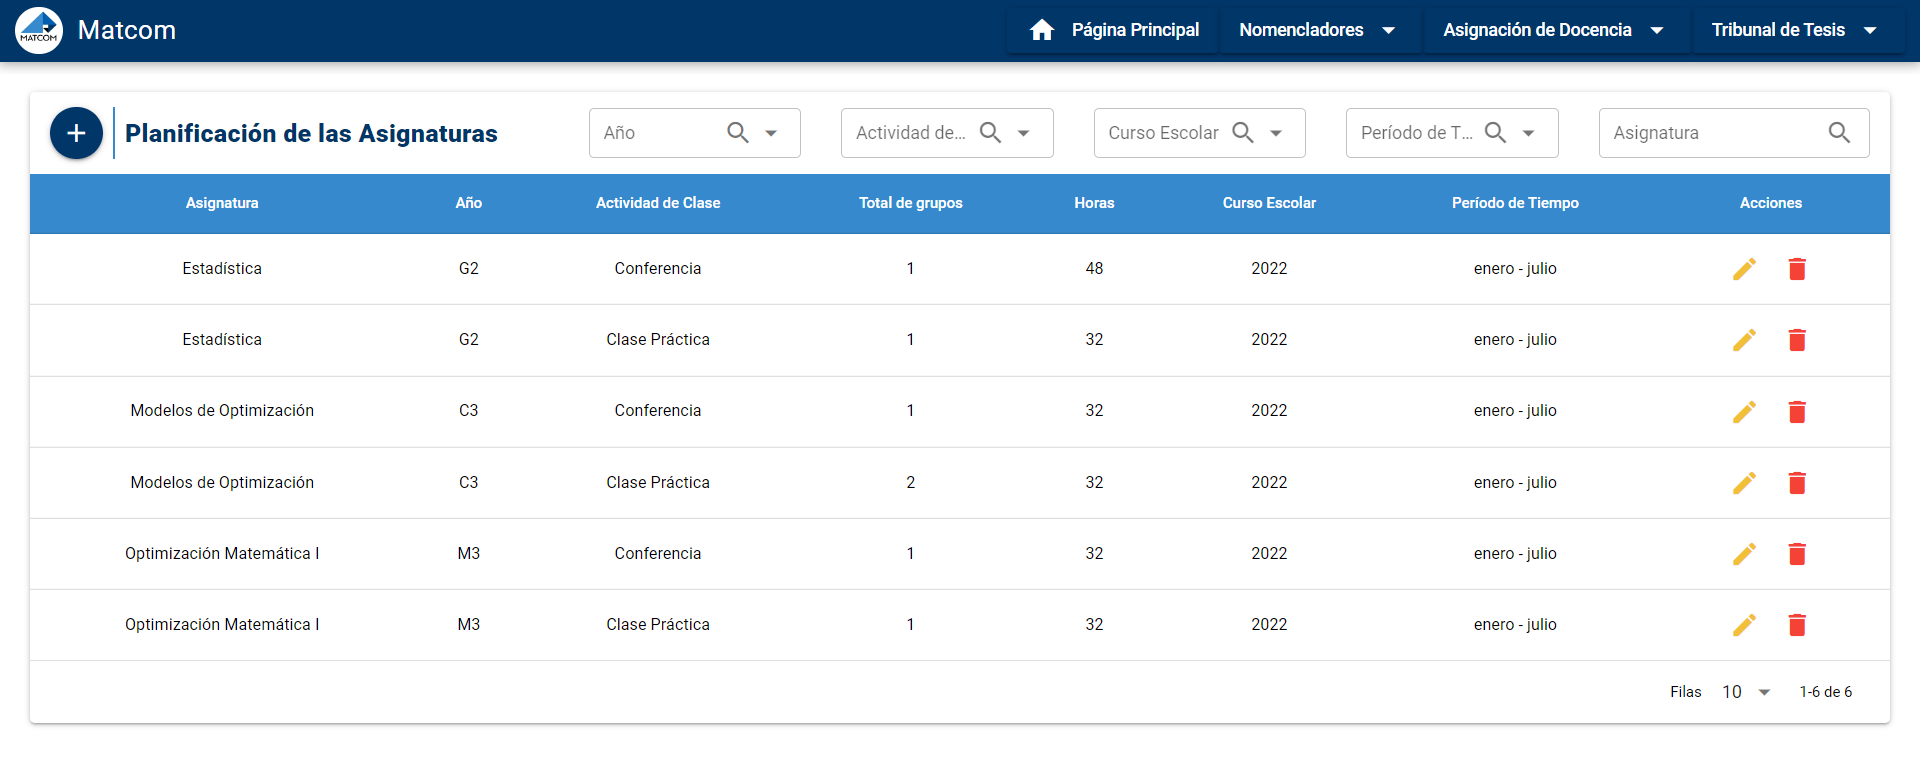
\includegraphics[scale=0.3]{Graphics/Implementation/Docencia/PD-result.png}
    \caption{Vista de la carga de las asignaturas}
    \label{img-pd-result}
\end{figure}

Por cada carga de asignatura que se agregue en el sistema se crean $n$ asignaciones 
de docencia sin asignar, donde $n$ es la cantidad de grupos que tiene la carga de la asignatura. En 
la figura \ref{img-ta-unassing} se muestran las asignaciones de docencias creadas automáticamente por el sistema 
a partir de las cargas agregadas en la figura \ref{img-pd-result}.

\begin{figure}[H]
    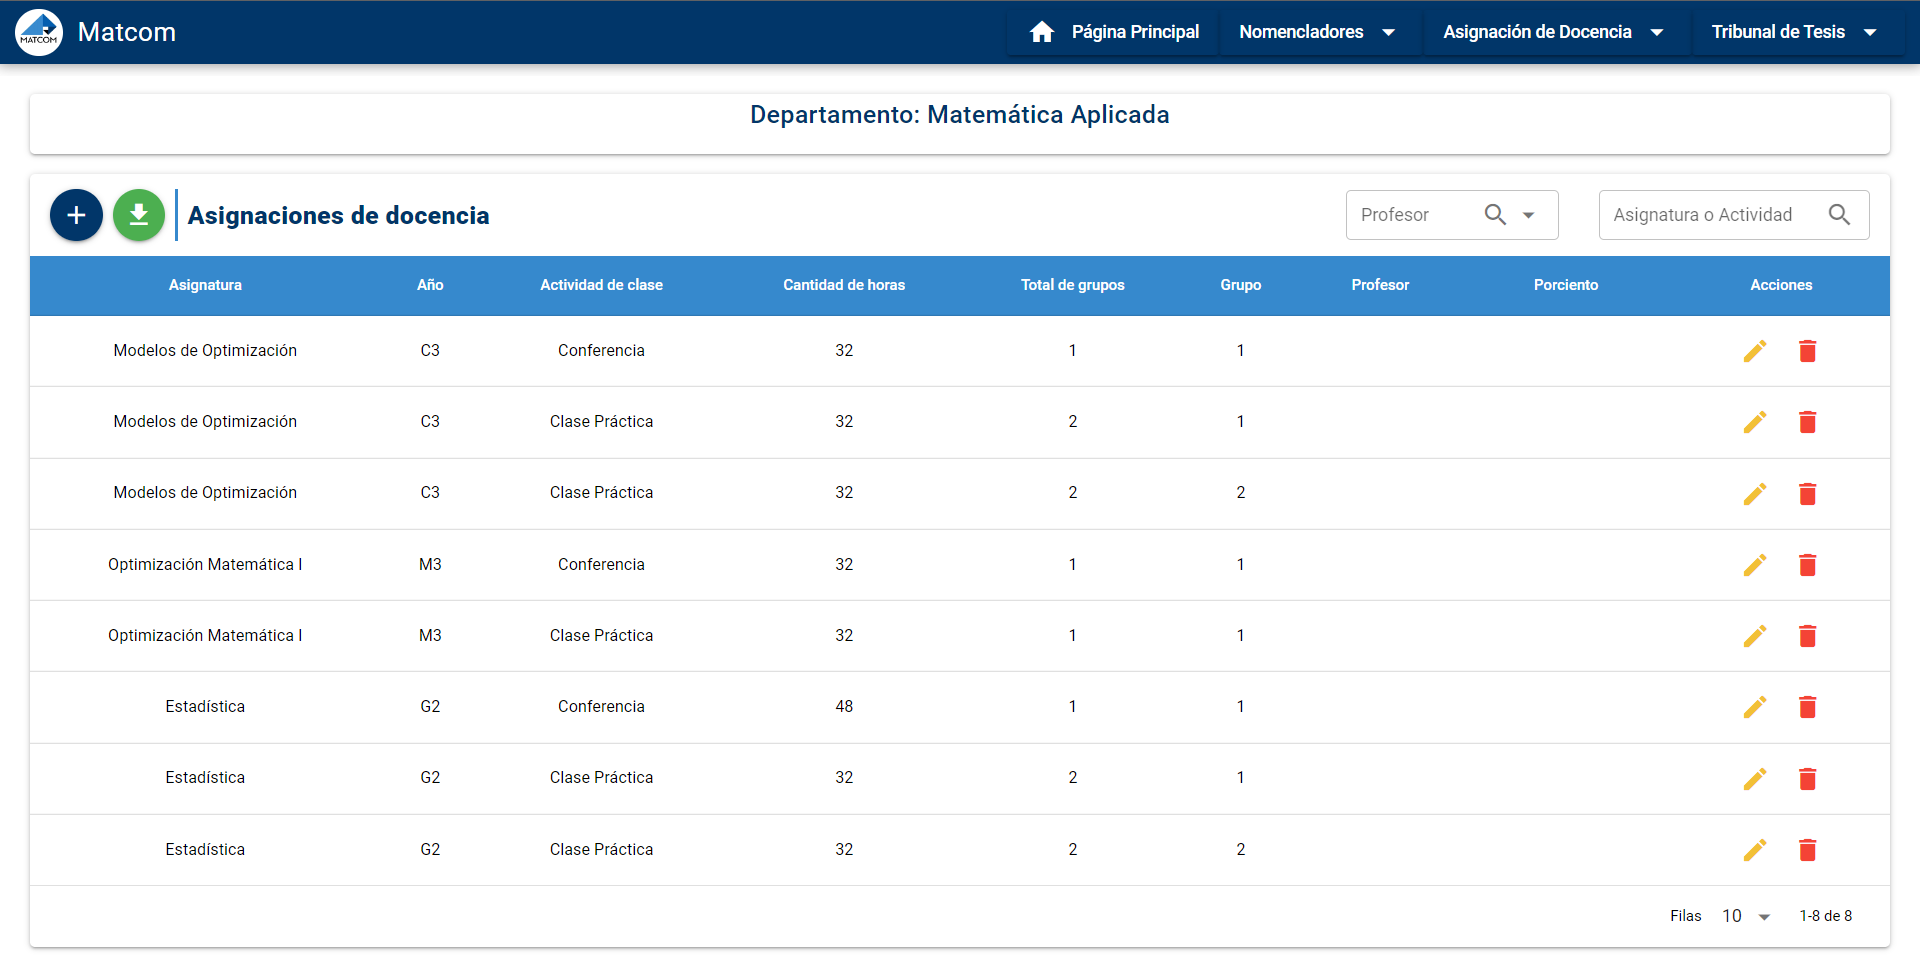
\includegraphics[scale=0.3]{Graphics/Implementation/Docencia/AD-unassing.png}
    \caption{Vista de la asignación de docencia}
    \label{img-ta-unassing}
\end{figure}


El próximo paso es realizar la asignación de los profesores para cubrir 
la docencia del semestre. Para asignar un profesor se debe 
pulsar sobre el botón de editar de una fila. En la figura \ref{img-ta-form-empty} se muestra el resultado 
de pulsar sobre el botón de editar de la cuarta fila, correspondiente a las conferencias
de la asignatura de Optimización Matemática I. 


\begin{figure}[H]
    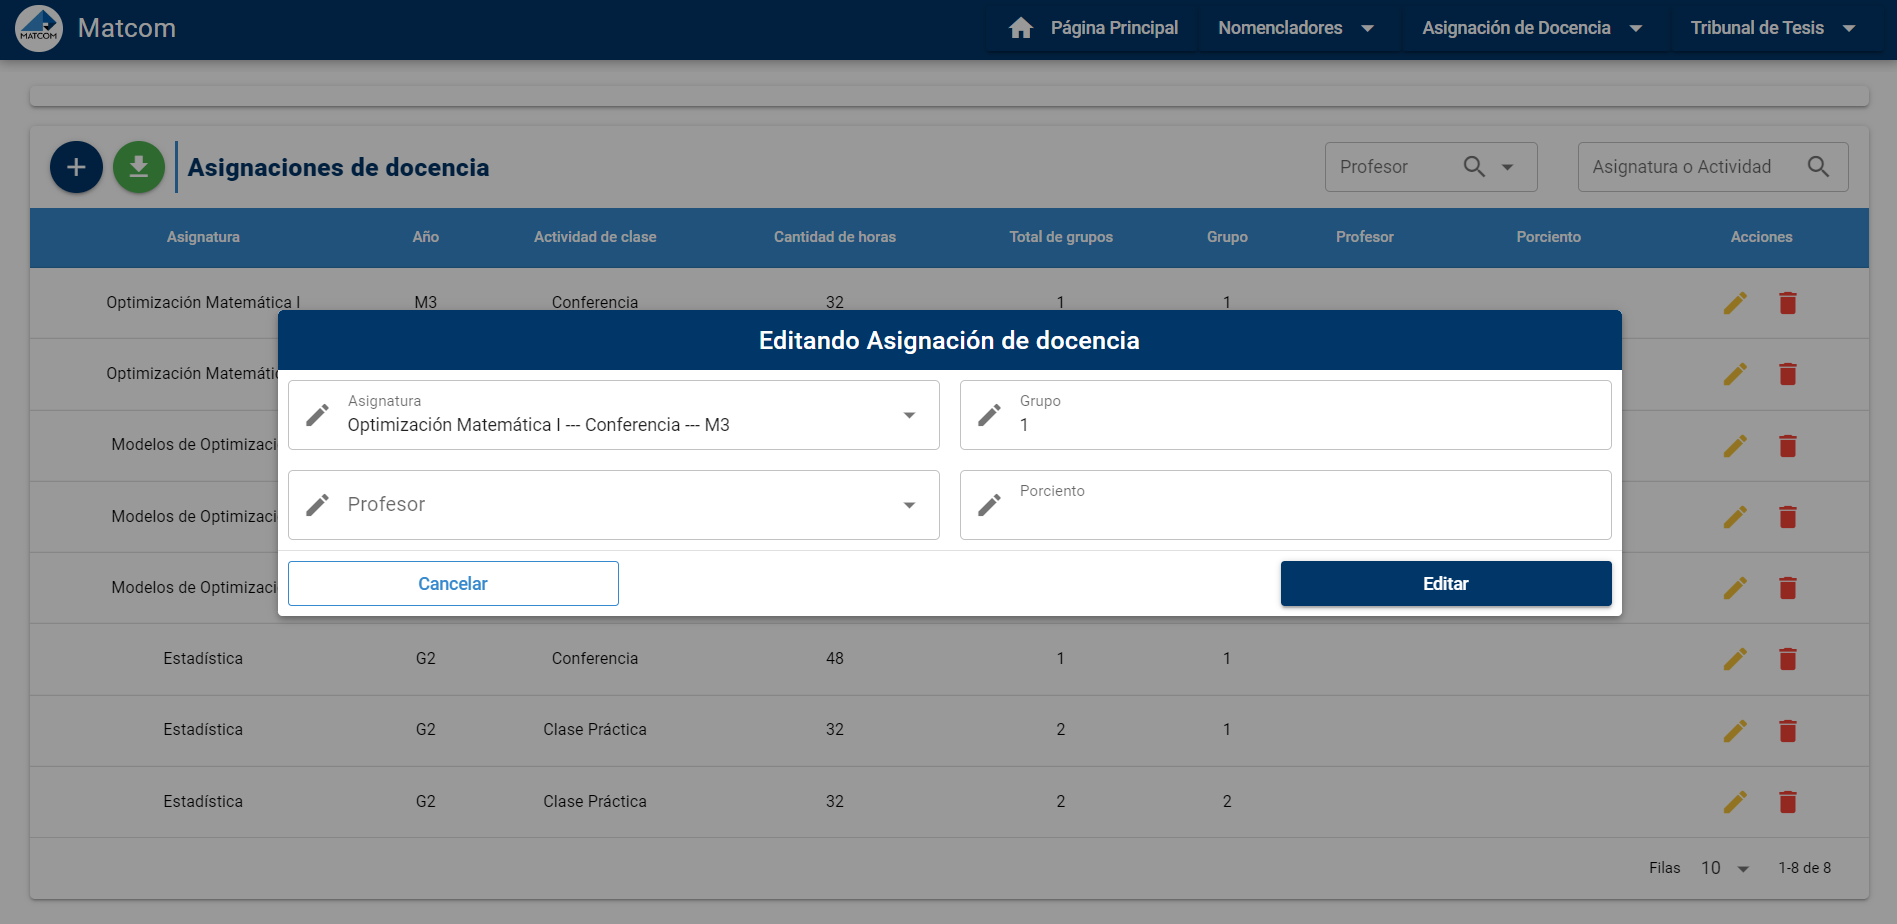
\includegraphics[scale=0.3]{Graphics/Implementation/Docencia/AD-form-empty}
    \caption{Vista del formulario para realizar una asignación de docencia}
    \label{img-ta-form-empty}
\end{figure}


Se deben completar los campos del formulario y pulsar sobre el botón editar. 
Como se muestra en la tabla \ref{tabla-asignación-cap4}, la profesora Aymeeé Marrero es la encargada de 
impartir las 32 horas de conferencia de la asignatura Optimización Matemática I, por 
tanto se debe especificar que la profesora imparte el 100 porciento de las horas 
como se muestra en la figura \ref{img-ta-form-fill}.


\begin{figure}[H]
    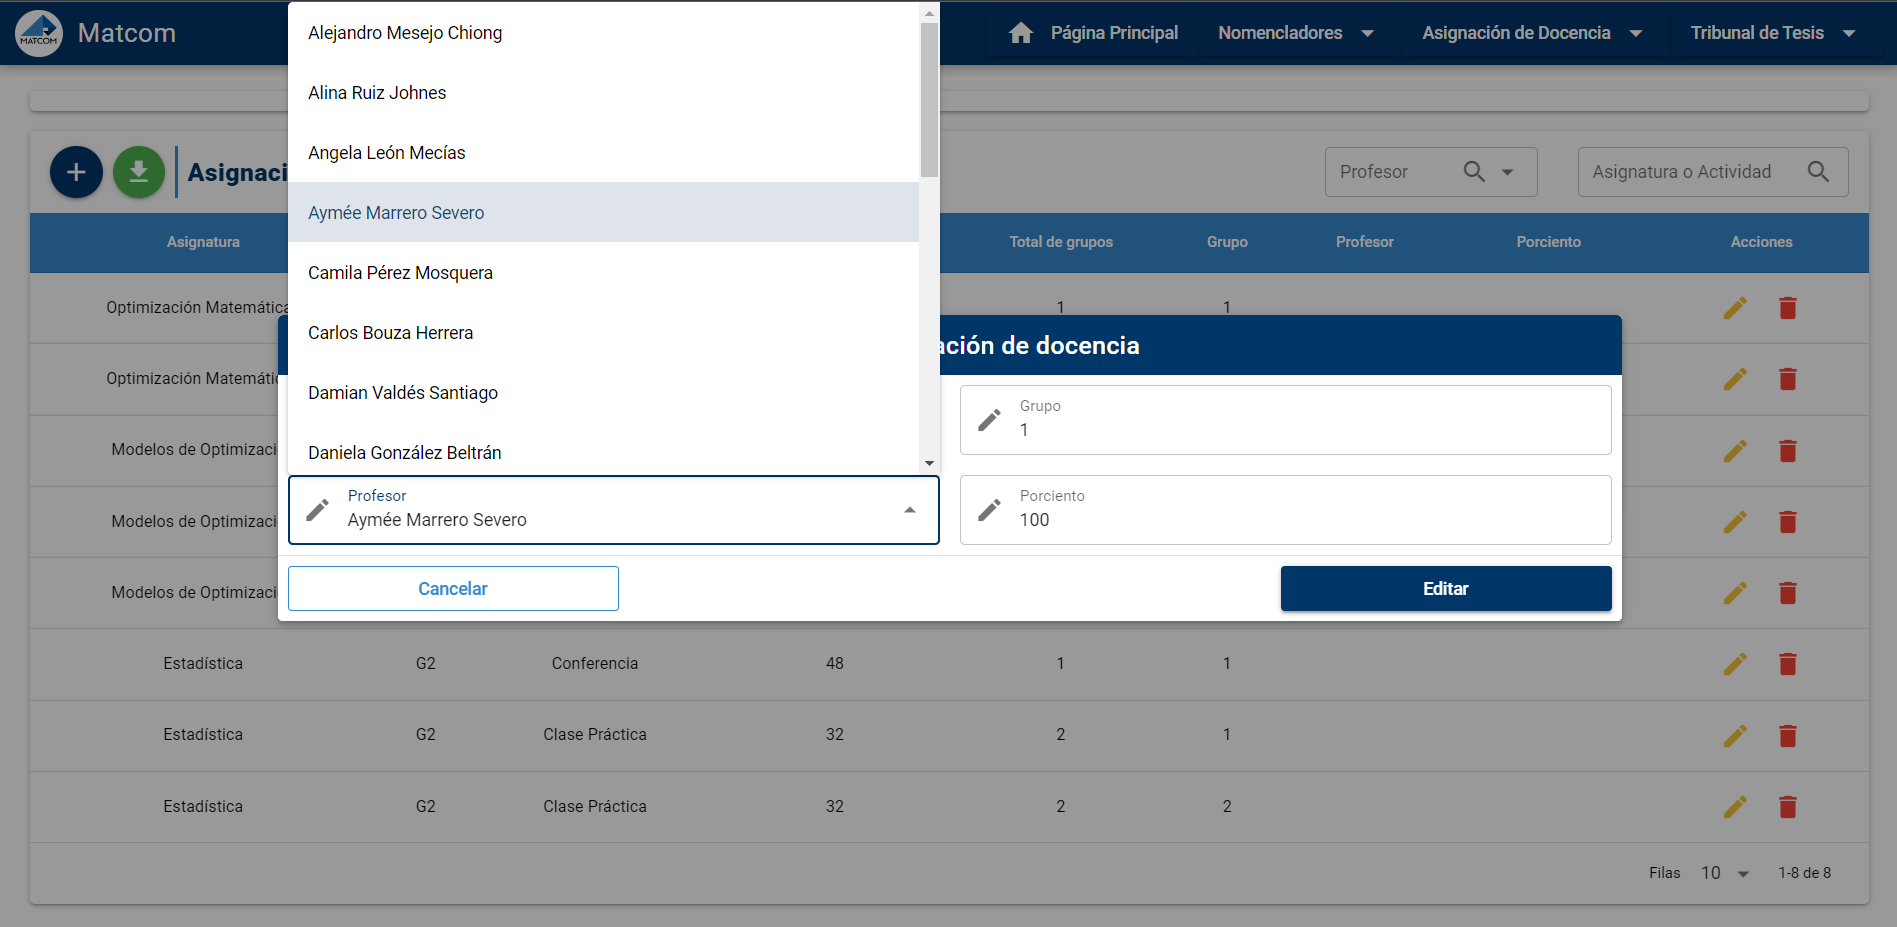
\includegraphics[scale=0.3]{Graphics/Implementation/Docencia/AD-form-fill.png}
    \caption{Vista del formulario con los datos ingresados de una asignación de docencia}
    \label{img-ta-form-fill}
\end{figure}


En la figura \ref{img-ta-one-assign} se muestra el resultado 
de realizar la asignación.


\begin{figure}[H]
    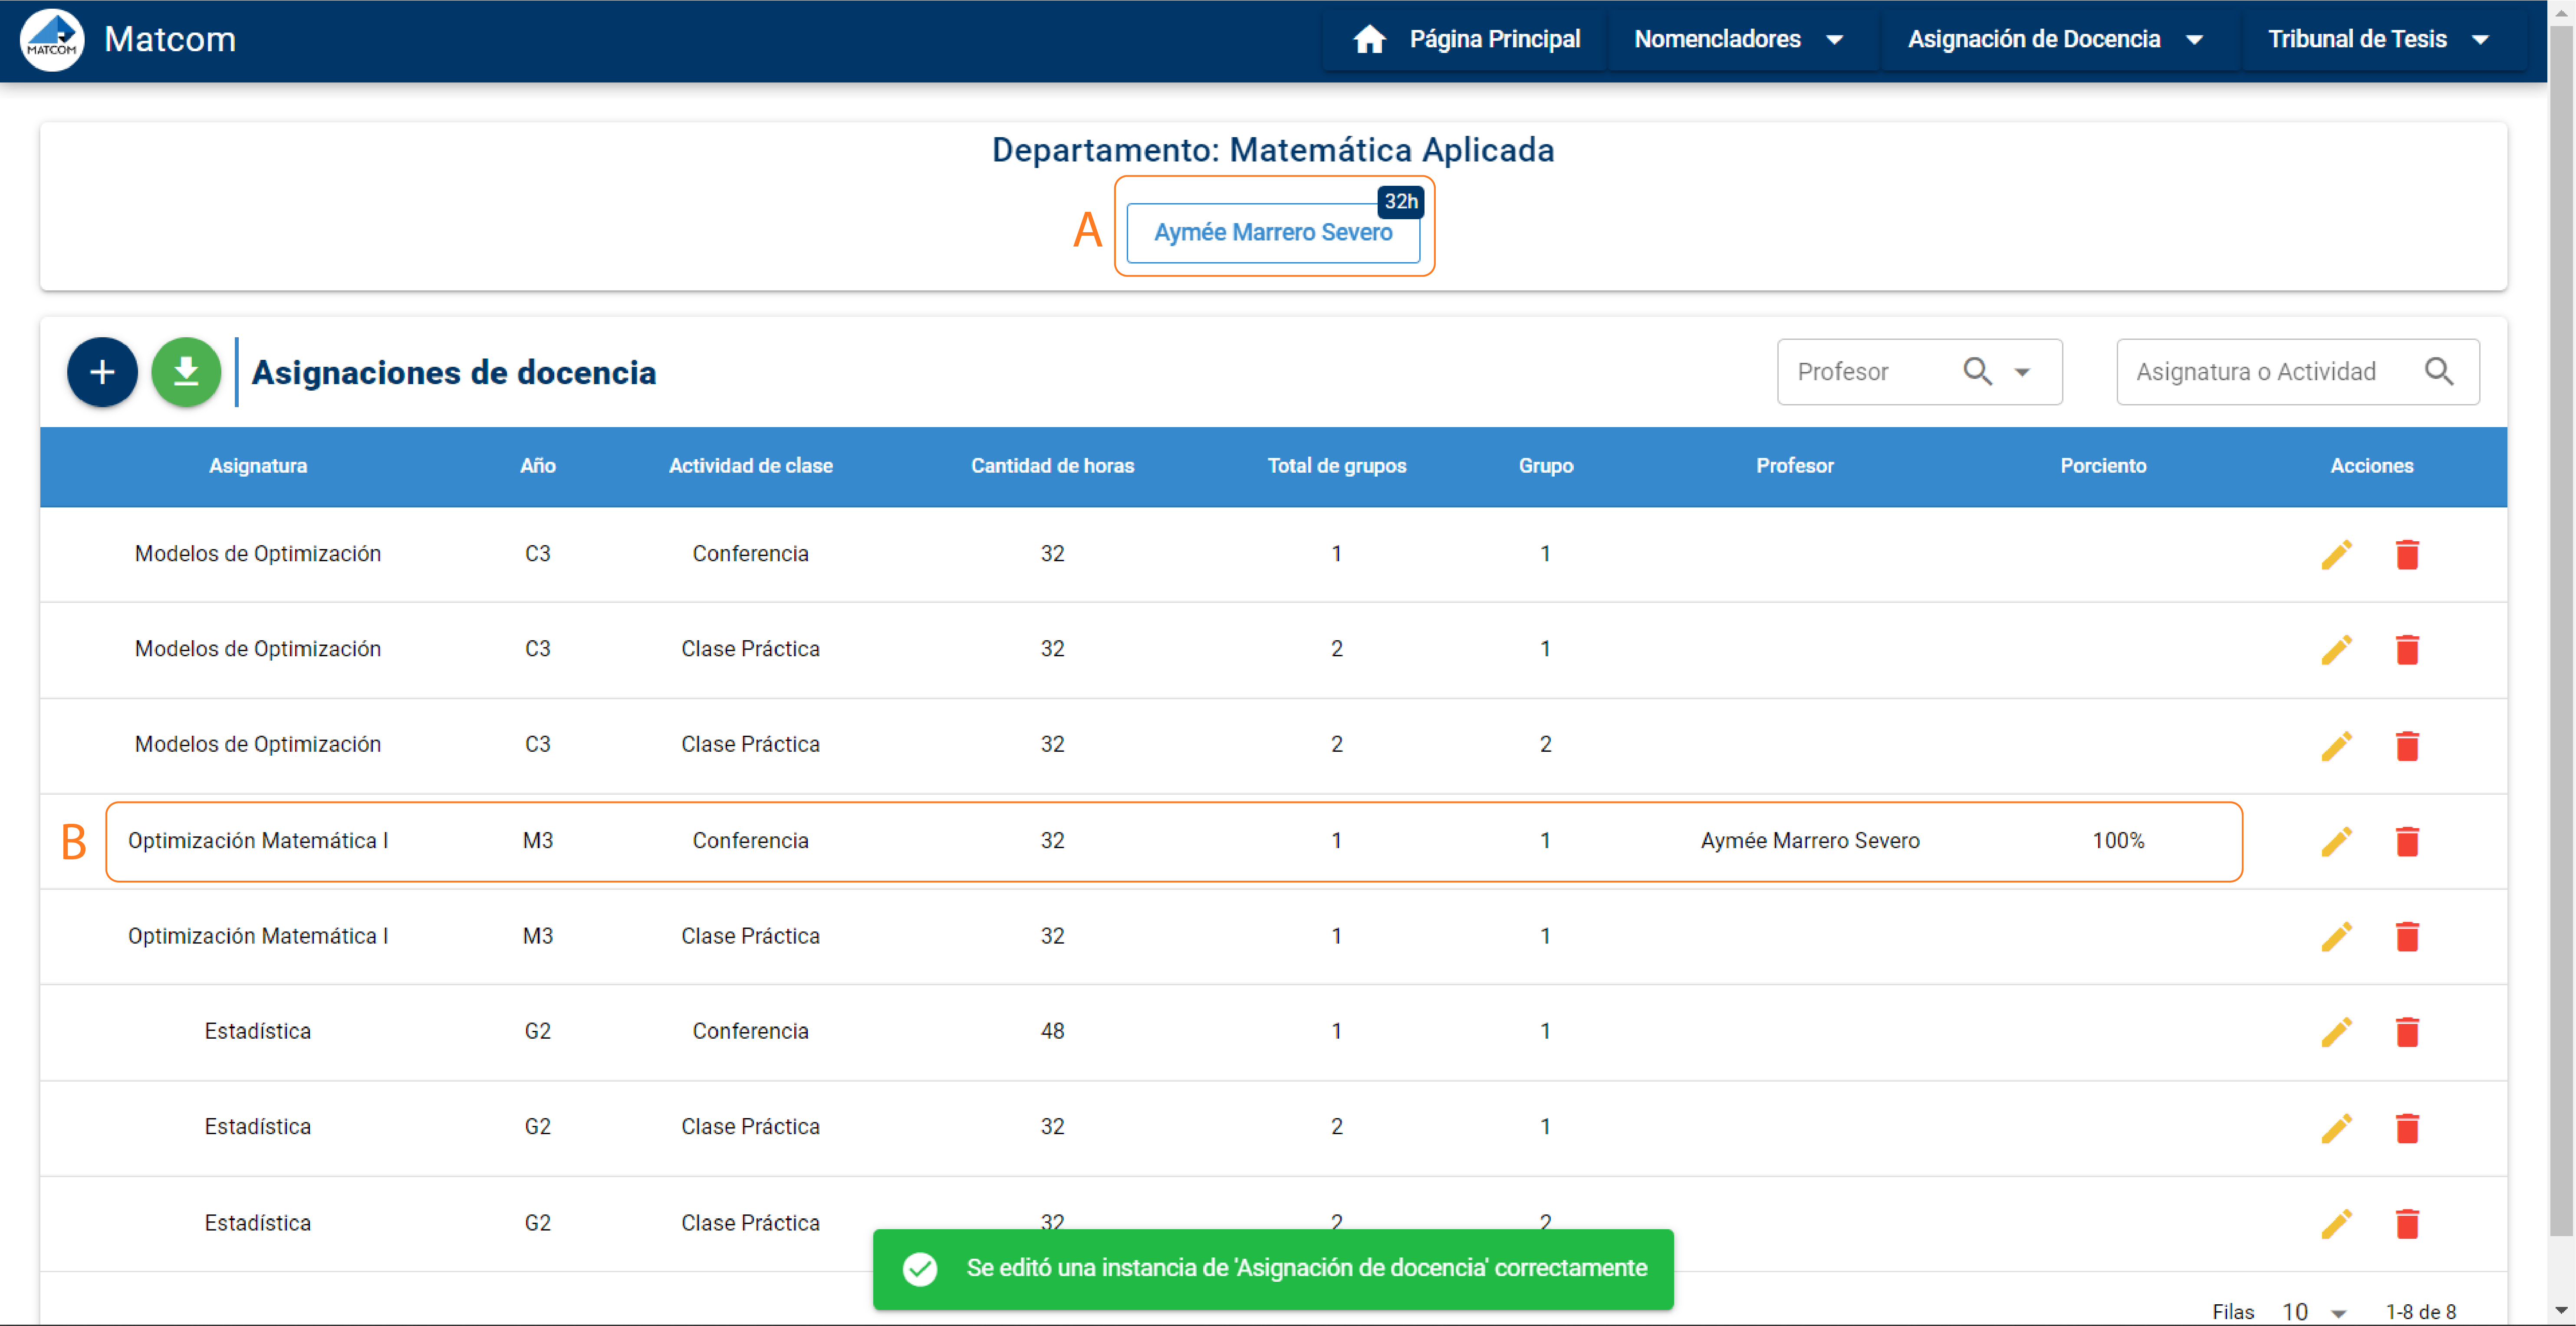
\includegraphics[scale=0.3]{Graphics/Implementation/Docencia/AD-one-assign.png}
    \caption{Vista resultante de realizar una asignación de docencia correctamente}
    \label{img-ta-one-assign}
\end{figure}

% Cada vez que se realicen cambios en la tabla, ya sean por agregar, editar o eliminar 
% asignaciones de docencia, la carga docente de los profesores se actualiza como se indica 
% en el recuadro A. El recuadro B refleja como quedó la fila tras la asignación de la profesora 
% Vivian Sistaschs para que imparta las 48 horas de conferencia de la asignatura Inferencia Matemática
% a los estudiantes que cursan el tercer año de la carrera Matemática.


Cada vez que se realicen cambios en la tabla, ya sean por agregar, editar o eliminar 
asignaciones de docencia, la carga docente de los profesores se actualiza como se indica 
en el recuadro A de la figura \ref{img-ta-one-assign}. El recuadro B refleja como quedó la fila tras la asignación de la profesora 
Aymeeé Marrero para que imparta las 32 horas de conferencia de la asignatura Optimización Matemática I
a los estudiantes que cursan el tercer año de la carrera Matemática.


En la figura \ref{img-ta-with-assign} se muestra el resultado de cubrir la docencia de las asignaturas de Optimización
Matemática I, Estadística y las clases prácticas de Modelos de Optimización, de acuerdo a la tabla \ref{tabla-asignación-cap4}.


\begin{figure}[H]
    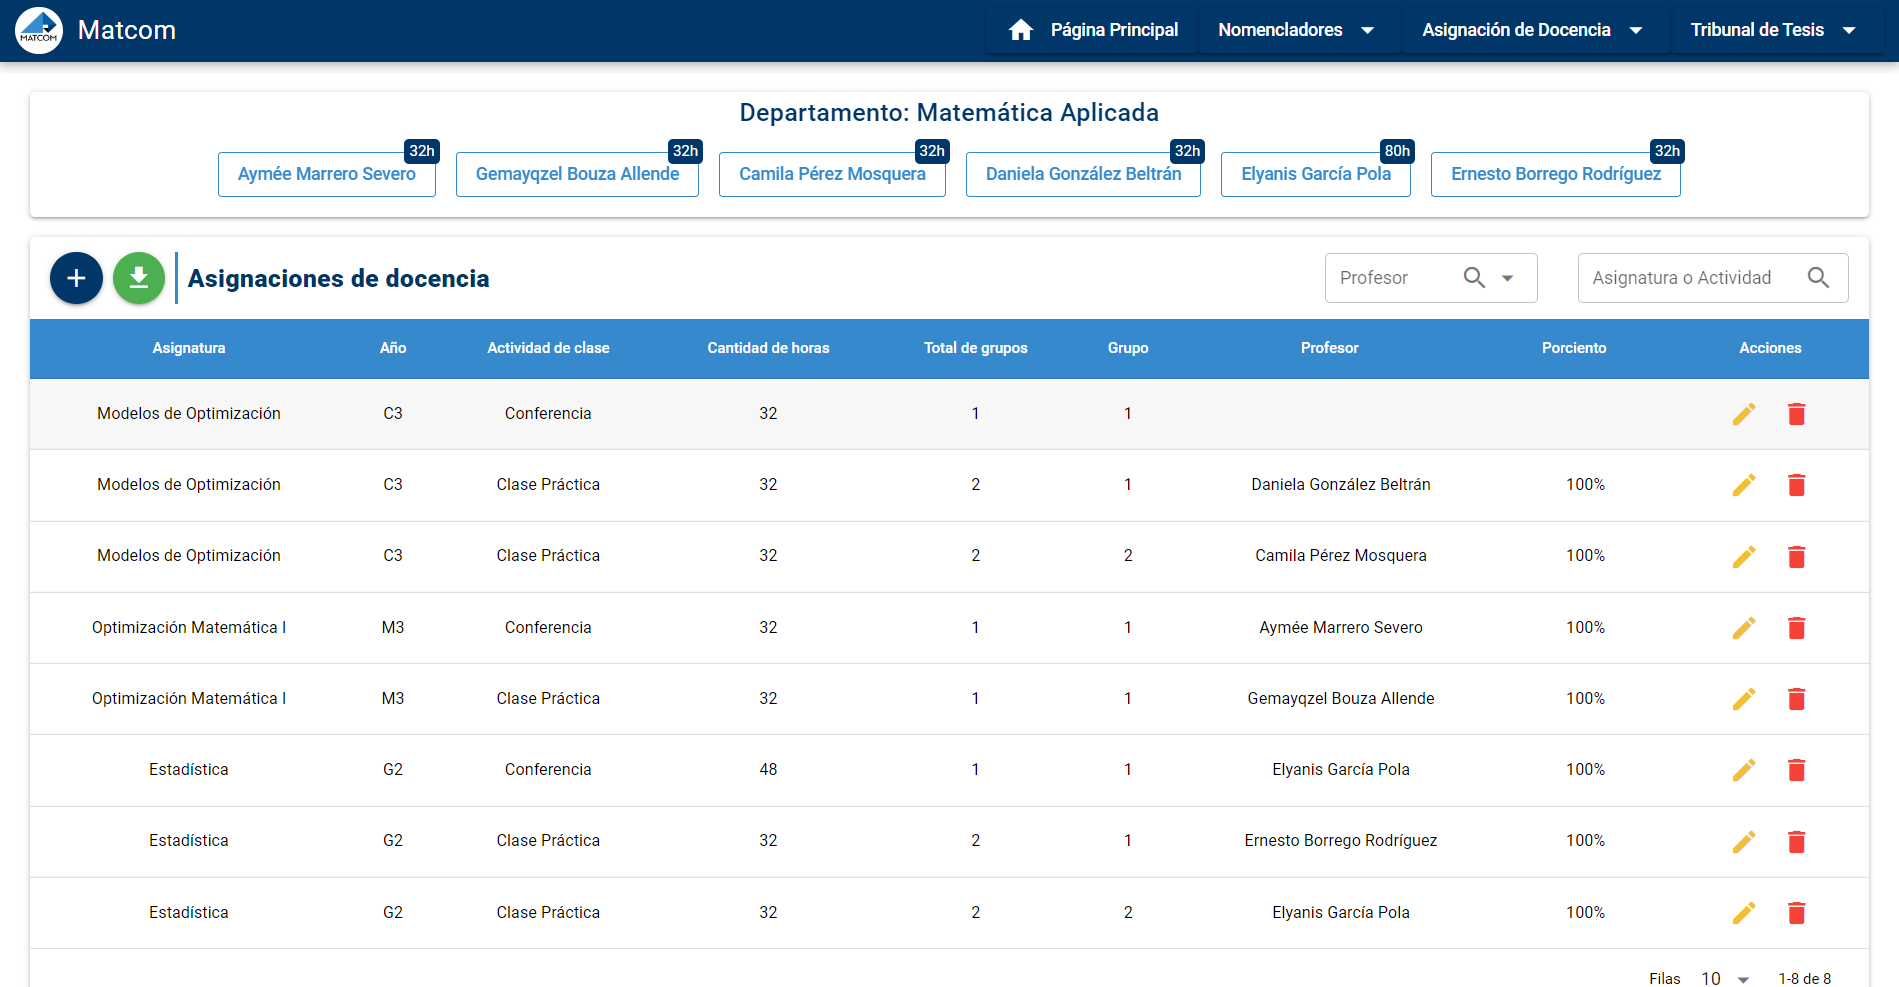
\includegraphics[scale=0.3]{Graphics/Implementation/Docencia/AD-with-assigns.png}
    \caption{Vista con varias asignaciones de docencia}
    \label{img-ta-with-assign}
\end{figure}


Las conferencias de la asignatura Modelos de Optimización I, se imparten por los profesores 
Aymeeé Marrero y Fernando Rodríguez, con 16 horas cada uno.
Para modelar esta distribución en el sistema, es necesario agregar una 
nueva asignación de docencia y especificar que cada profesor va a impartir el 50 porciento 
de las horas totales de conferencia. Para agregar una nueva asignación se debe pulsar sobre el 
botón de agregar y llenar los campos necesarios. En la figura
\ref{img-ta-result}, se muestra como queda
la asignación final de la docencia. 

\begin{figure}[H]
    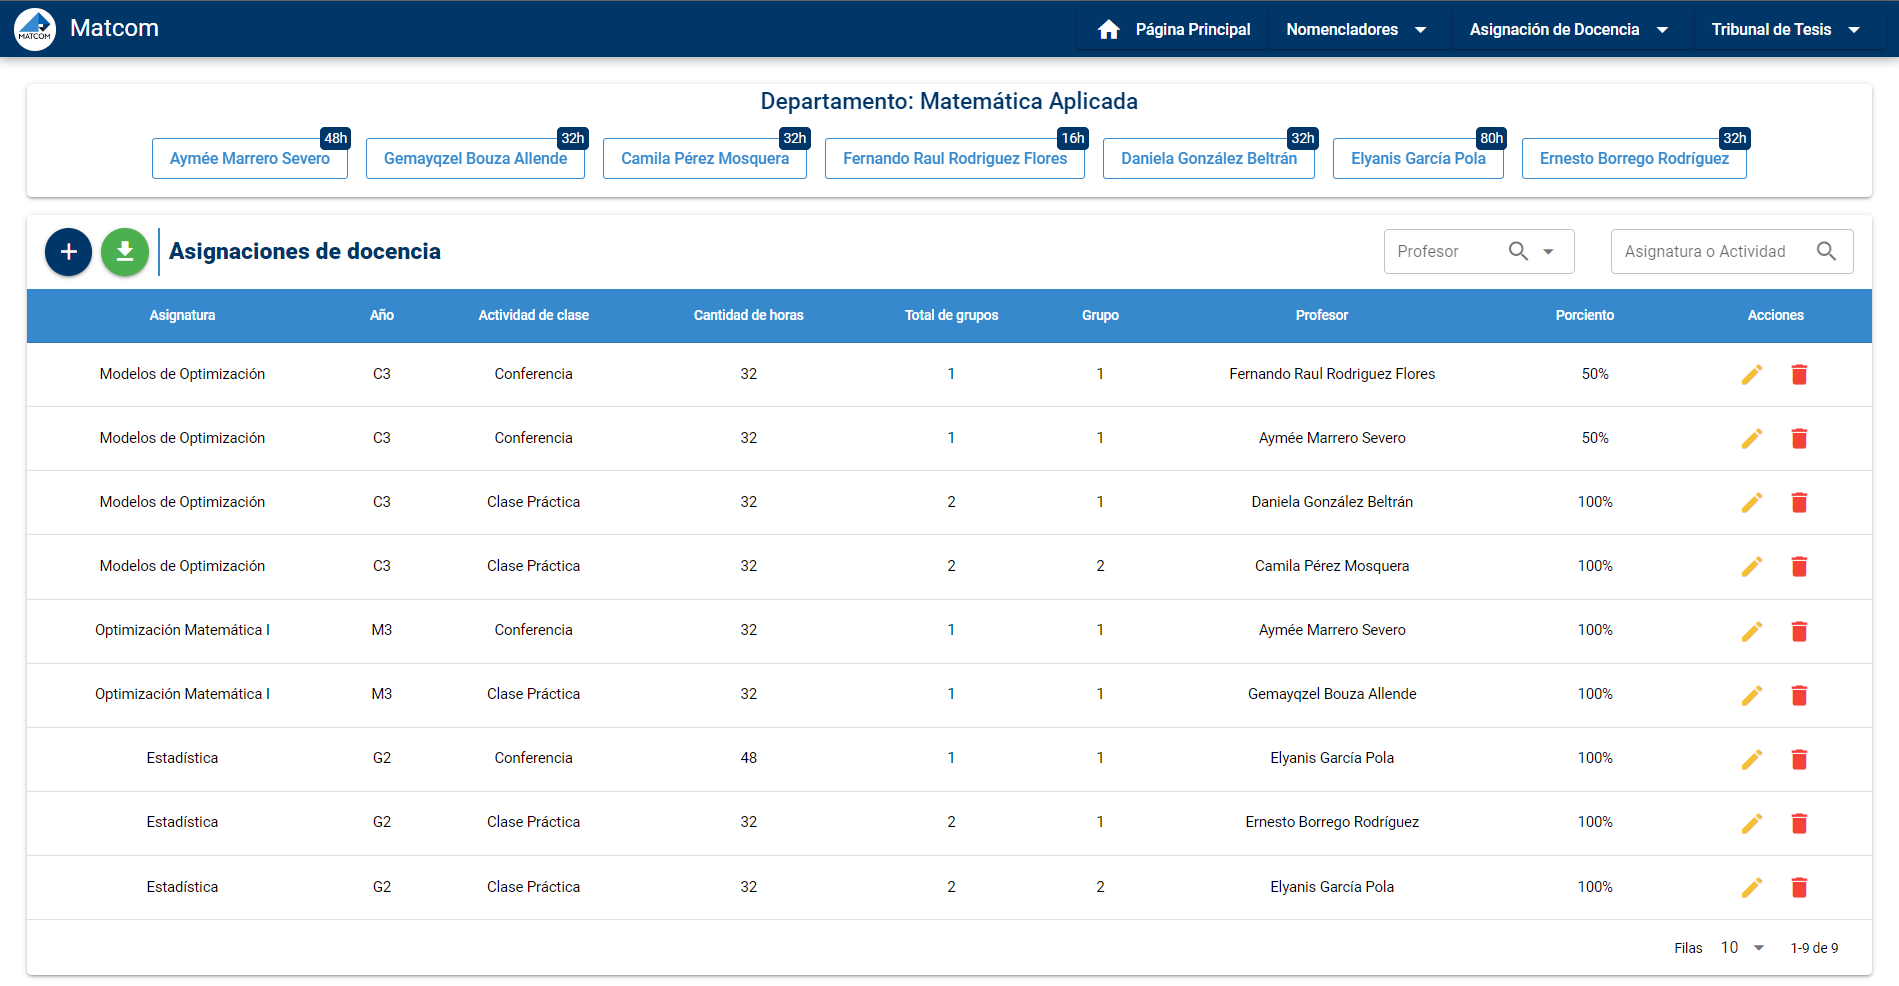
\includegraphics[scale=0.3]{Graphics/Implementation/Docencia/AD-result.png}
    \caption{Vista resultado de la asignaciones de docencia}
    \label{img-ta-result}
\end{figure}


Para poder llevar a cabo el proceso de asignación de docencia a través del sistema 
que se propone, es necesario que en la base de datos se ingresen las informaciones 
que intervienen en este proceso. Por ejemplo, para realizar una asignación de docencia se necesitan 
los profesores del departamento
y las planificaciones de las cargas de las asignaturas. Para poder crear las cargas  
se necesitan las asignaturas, los años escolares, las actividades de clase y los períodos de tiempo.
Por tanto el primer paso para realizar la asignación de docencia es ingresar todos los datos que 
se describen en la sección \ref{database:asignación-docencia}.







% El proceso de asignación de docencia en un departamento se realiza en la 
% interfaz que se muestra en la figura \ref{img-ta-done}. El usuario de la 
% aplicación puede ver la carga docente de los profesores durante el proceso 
% de asignación, realizar filtrados por profesor para ver las asignaturas 
% que tiene asignada y descargar un documento CSV que contiene la información 
% de la docencia una vez haya terminado la asignación.


% \begin{figure}[H]
%     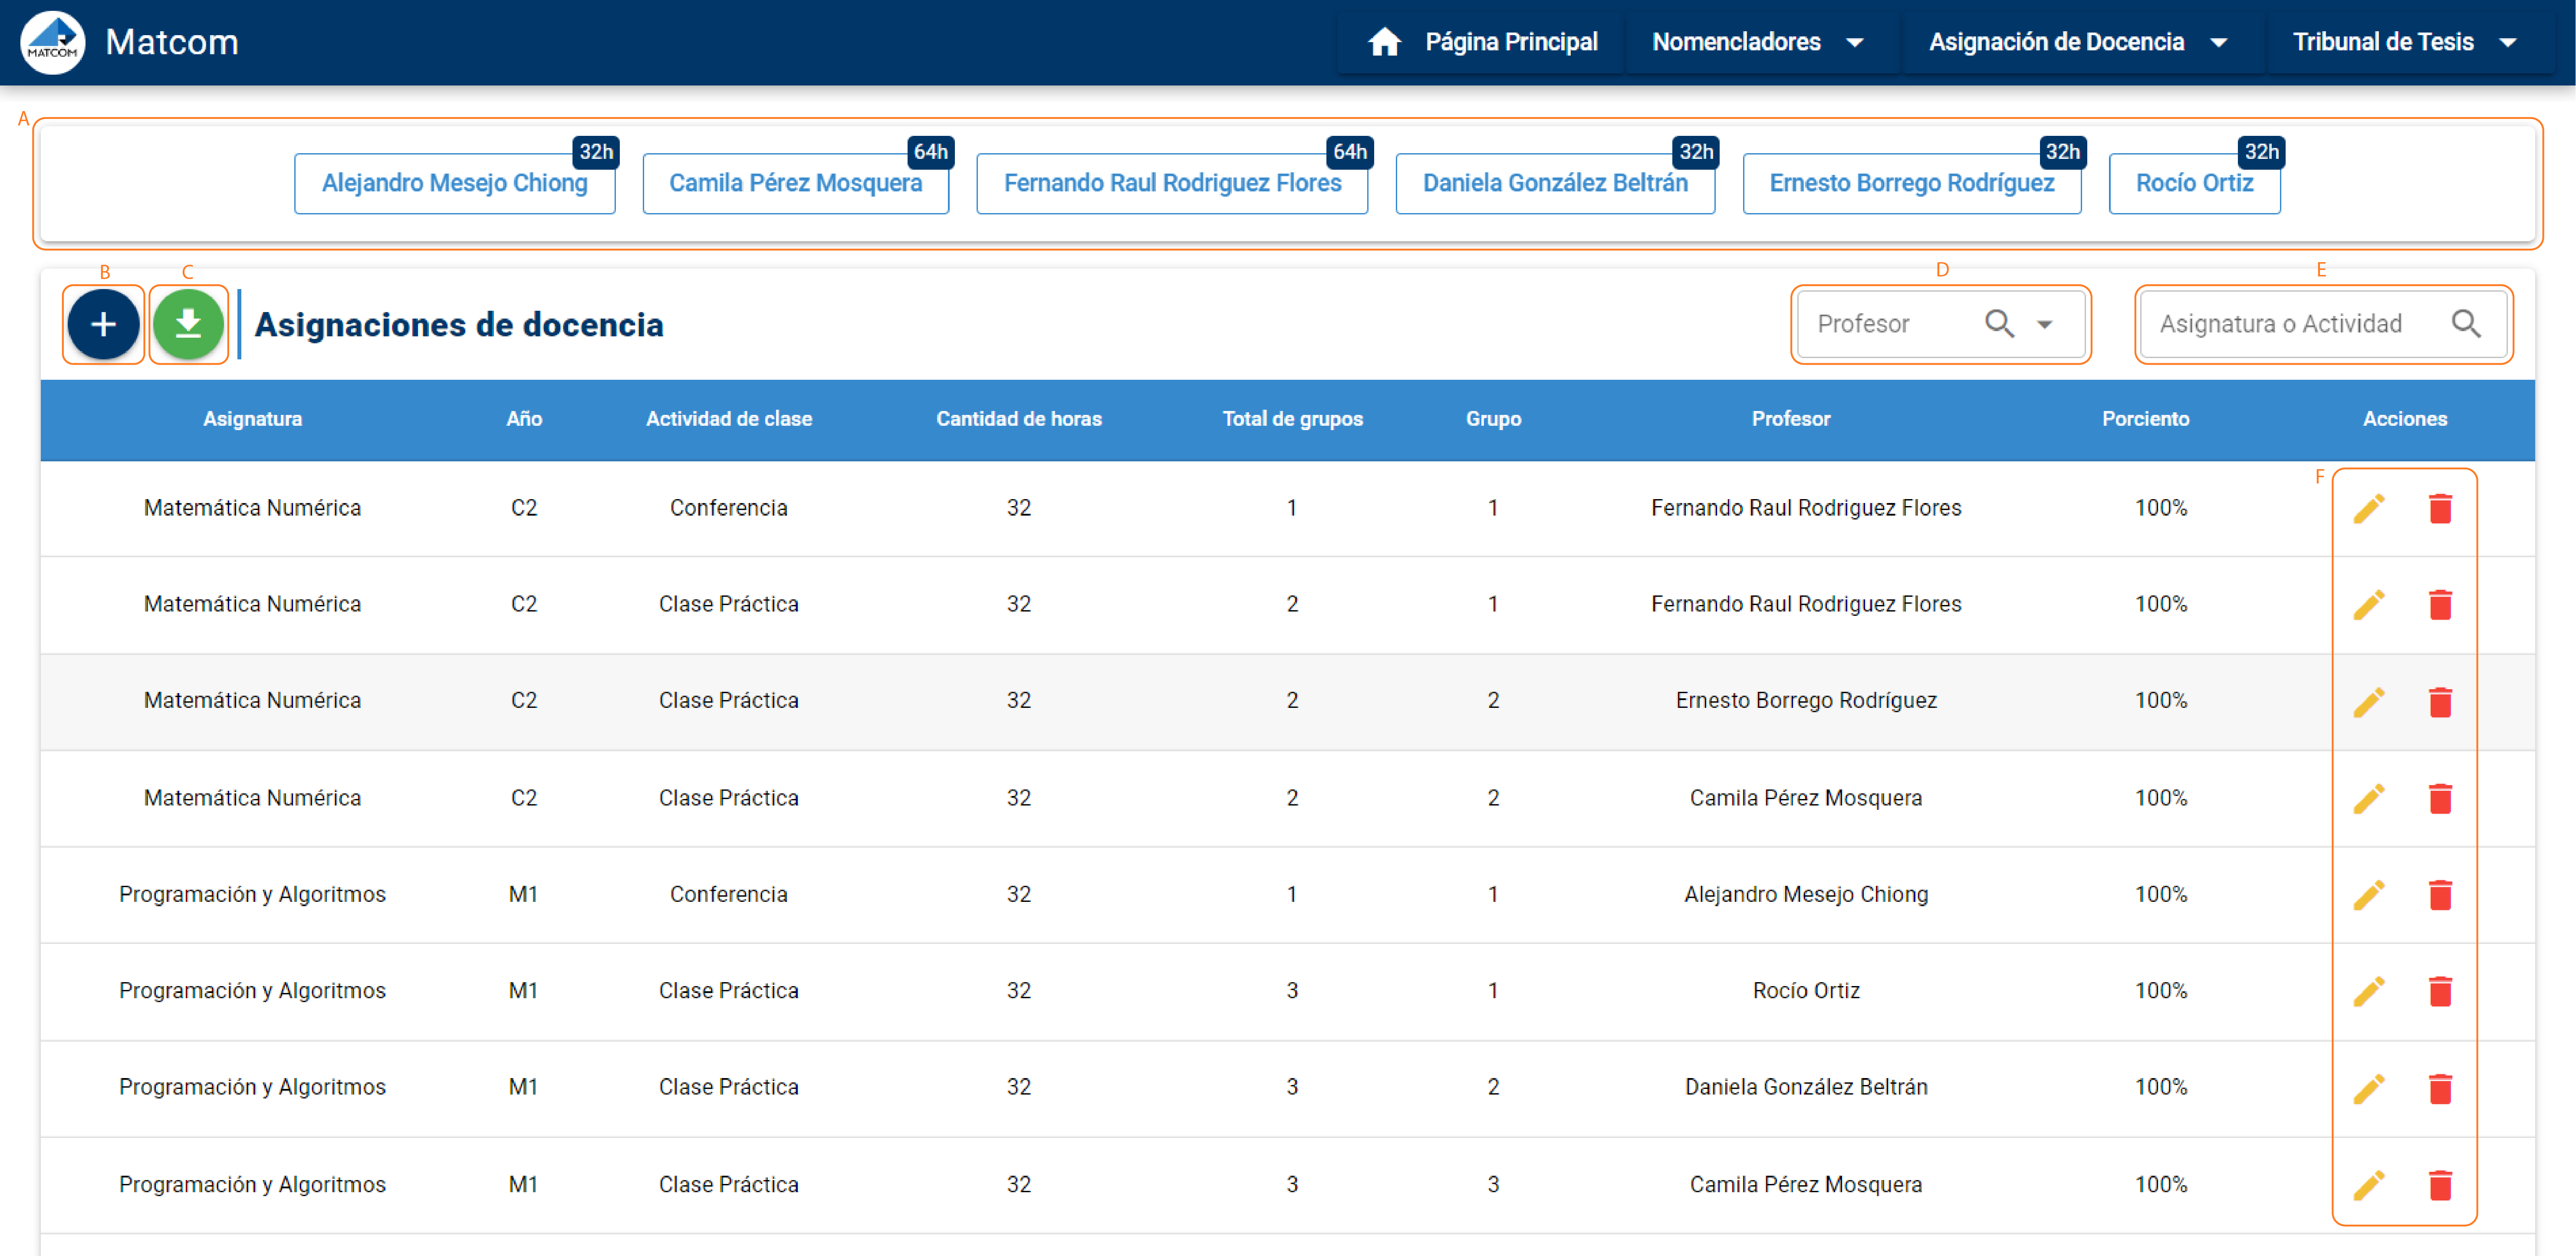
\includegraphics[scale=0.3]{Graphics/Implementation/Docencia/AD-asignada.png}
%     \caption{Vista de la asignación de docencia}
%     \label{img-ta-done}
% \end{figure}

% En la figura \ref{img-ta-done},
% se indican con recuadros cuatro regiones cuyo significado se explica a continuación.

% \begin{itemize}
%     \item A: muestra la carga docente de los profesores dada la asignación actual.
%     \item B: botón para agregar una nueva planificación de docencia.
%     \item C: botón para descargar la asignación de docencia actual.
%     \item D: realizar filtrado por los profesores para ver las asignturas que tiene asignadas.
%     \item E: realizar búsquedas por las asignaturas o actividades de clase.
%     \item F: botones para editar o borrar una fila de la tabla.  
% \end{itemize}



% En la figura \ref{img-ta-ordering} se muestra como quedaría ordenada la tabla a partir de los profesores,
% con el objetivo de mostrar primero aquellas 
% asignaturas que no se han asignado aún.


% \begin{figure}[H]
%     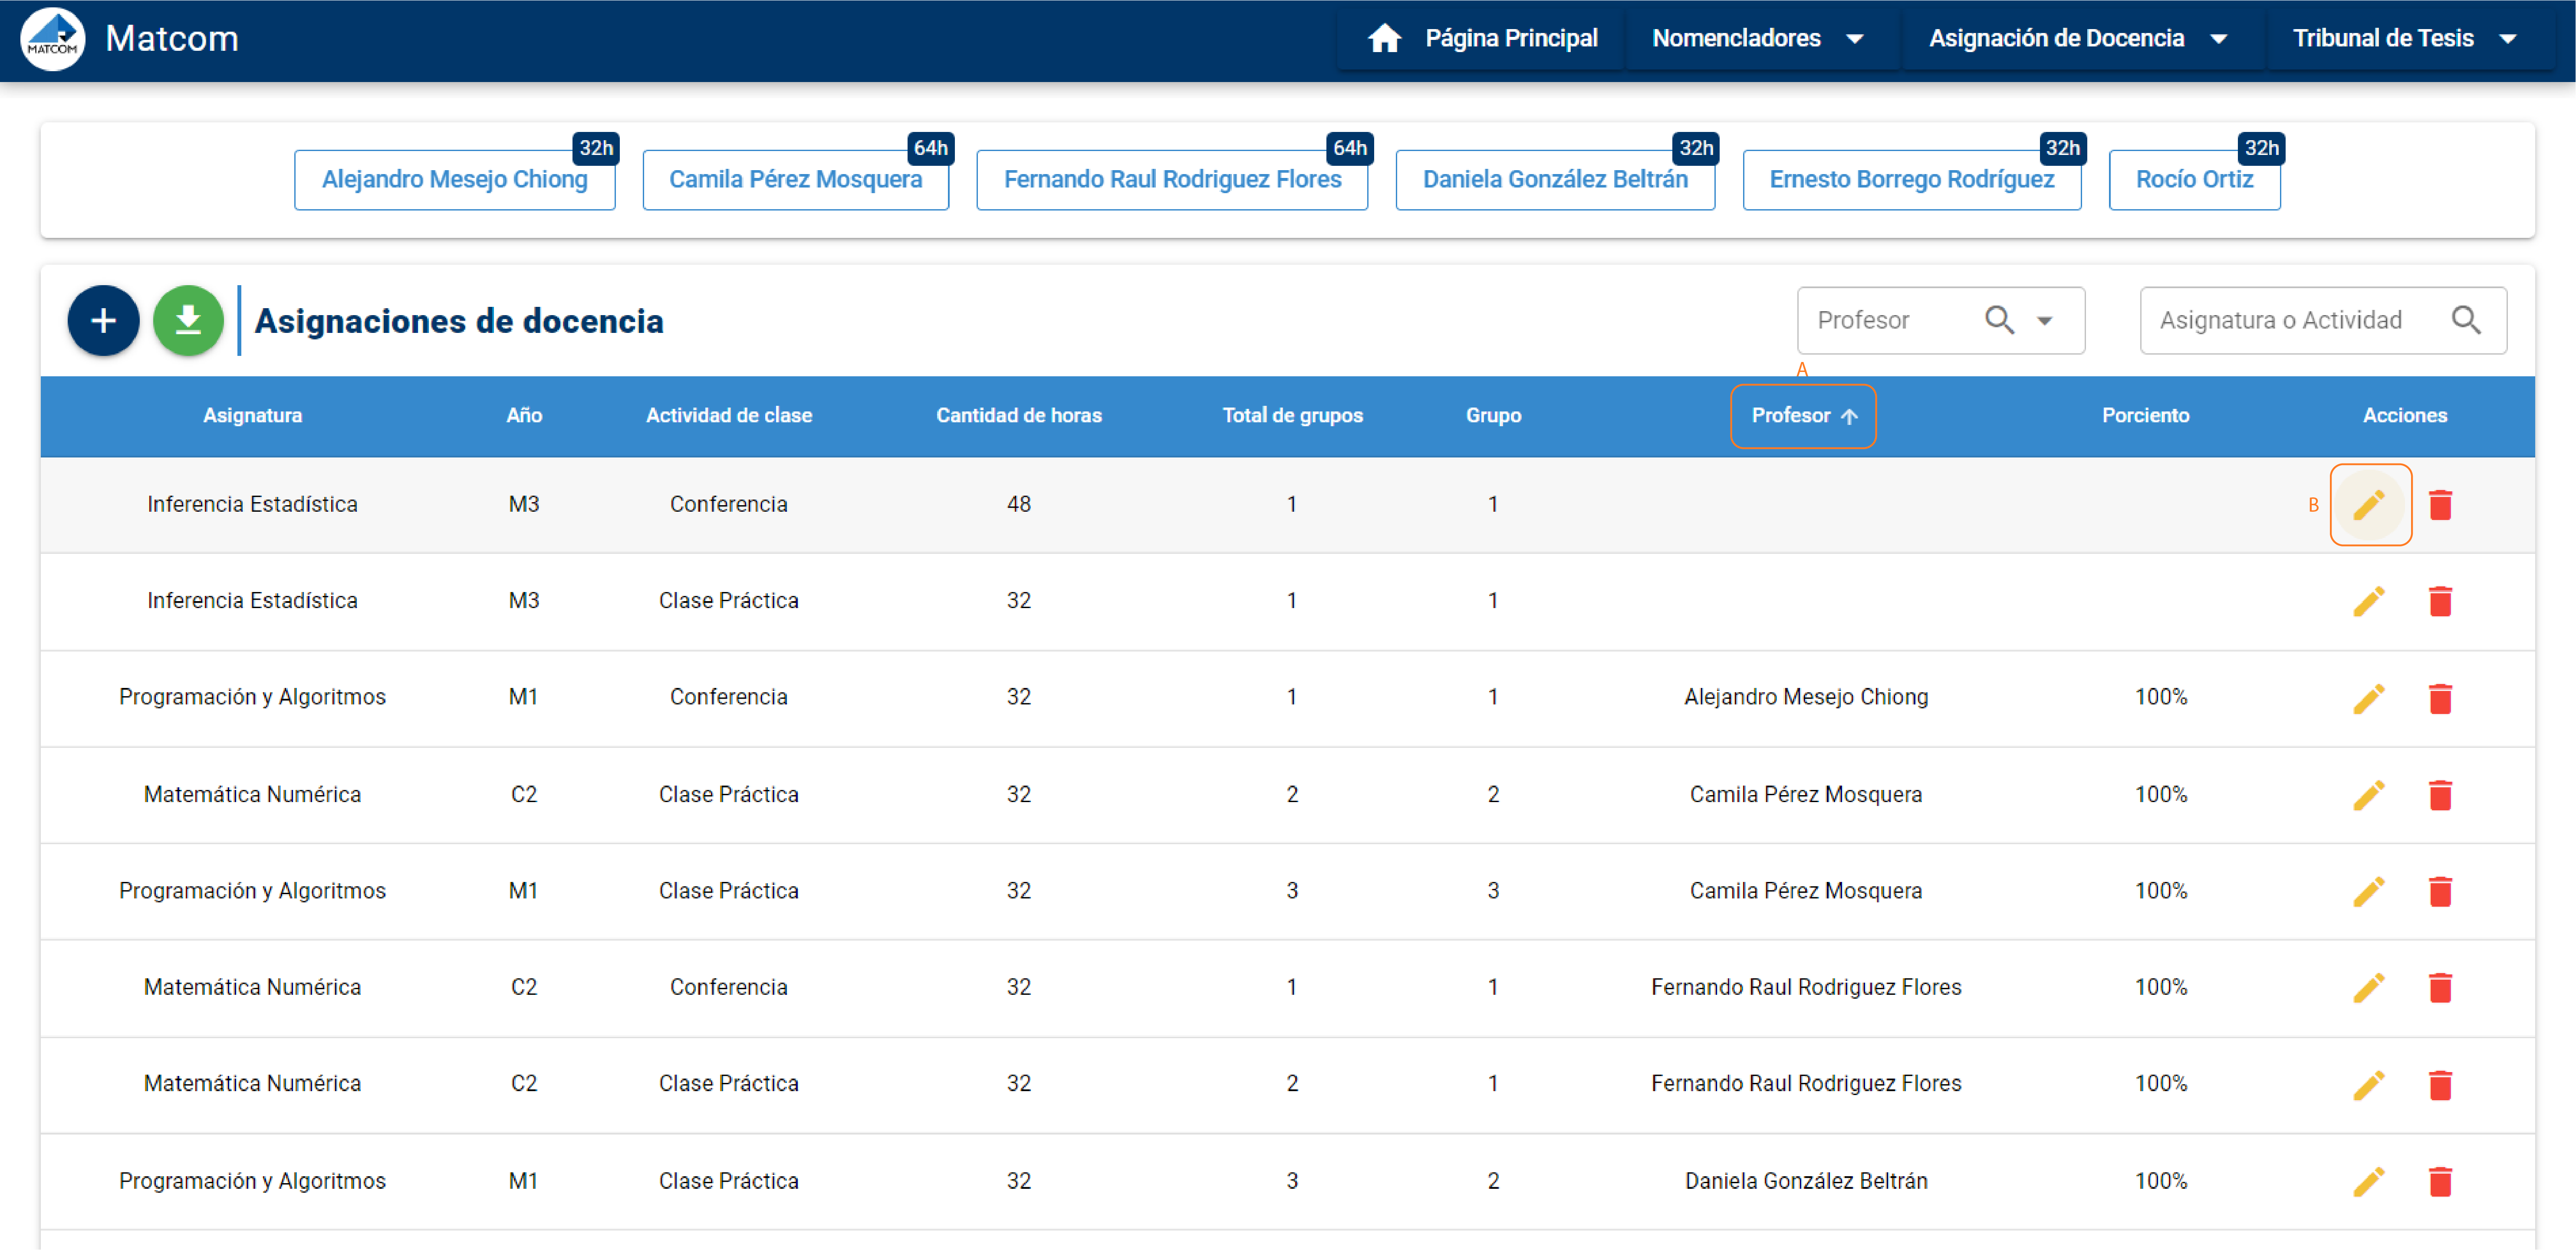
\includegraphics[scale=0.3]{Graphics/Implementation/Docencia/AD-sin-asignar.png}
%     \caption{Vista de la asignación de docencia, ordenada por profesores para que aparezcan primero las asignaturas que aún no han sido asignadas}
%     \label{img-ta-ordering}
% \end{figure}


% Para ordenar la tabla a partir de los profesores se debe pulsar sobre el elemento que se indica en 
% con el recuadro A. Para realizar una asignación se debe pulsar el botón de editar que se indica con
% con el recuadro B. La figura \ref{img-ta-edit-form1} muestra la vista después de pulsar el botón de 
% editar.  



% \begin{figure}[H]
%     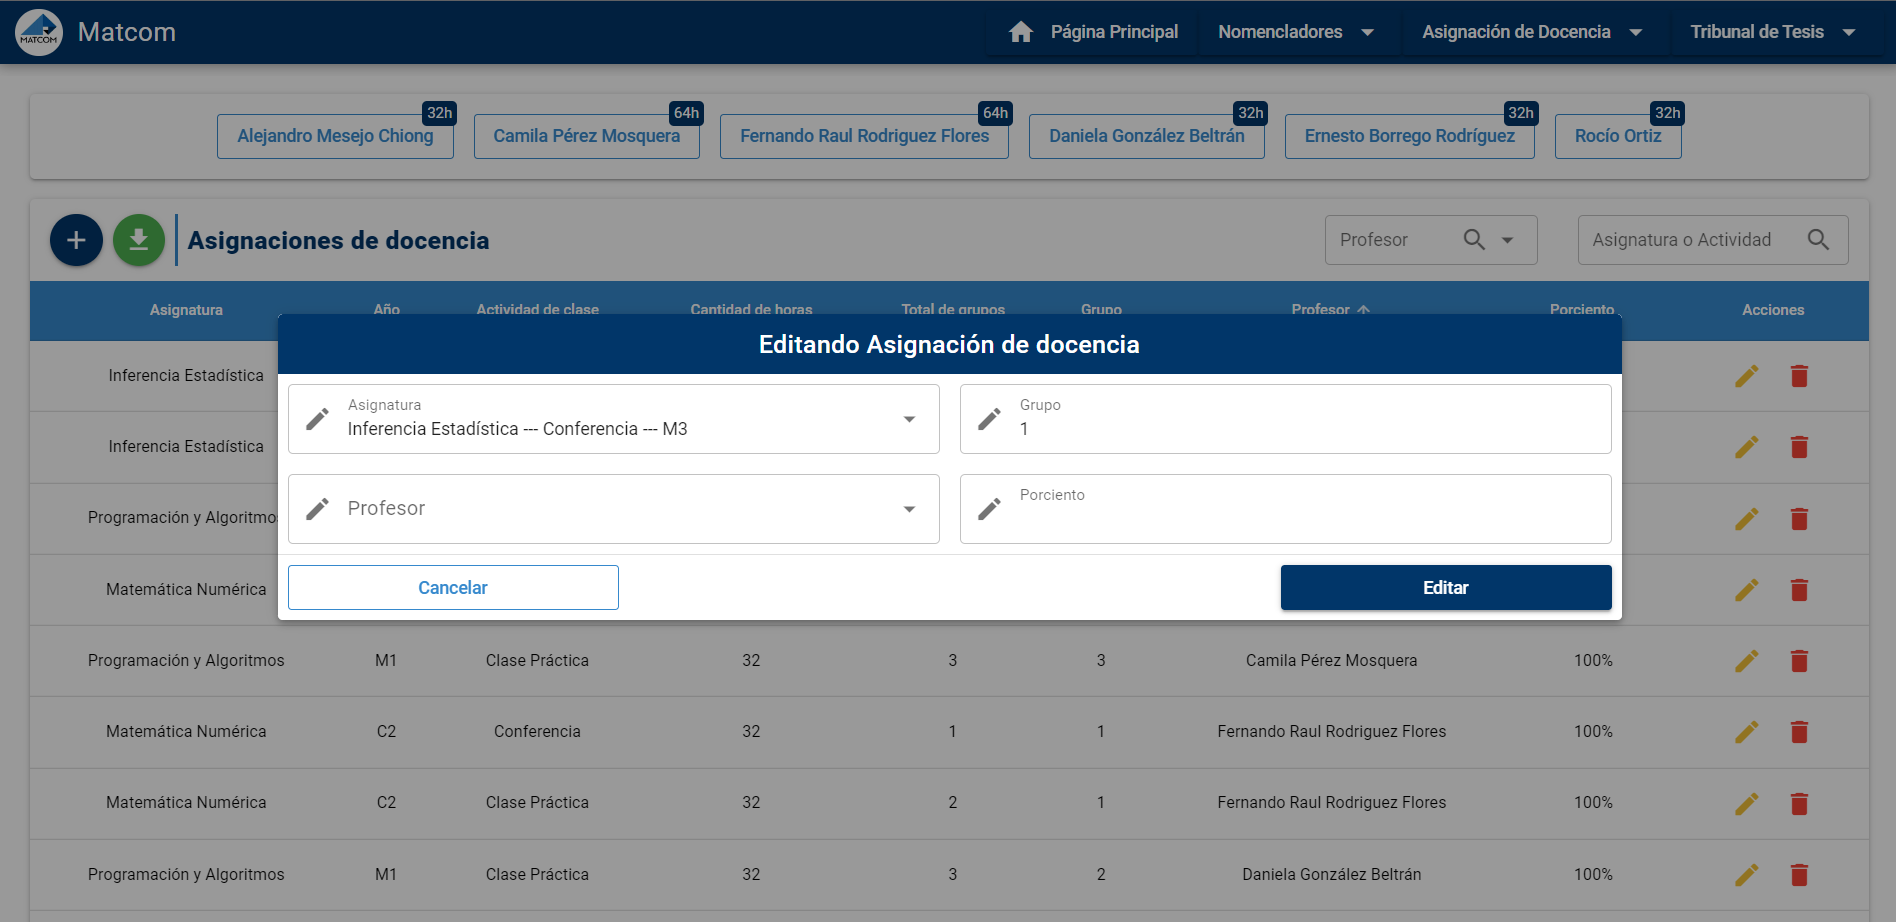
\includegraphics[scale=0.3]{Graphics/Implementation/Docencia/AD-edit-form.png}
%     \caption{Vista del formulario para editar una asignación de docencia}
%     \label{img-ta-edit-form1}
% \end{figure}


% Cuando se edita una asignación de docencia es necesario definir la planificación de 
% la asignatura (Inferencia Estadística---Conferencia---M3), grupo, profesor que se 
% desea asignar y el porciento total de horas que impartirá el profesor. En la figura
% \ref{img-ta-edit-form2} se muestra como asignar a la profesora Vivian Sistaschs con un 100
% porciento de las horas que se deben impartir en la planificación de la asignatura Inferencia Estadística. 

% \begin{figure}[H]
%     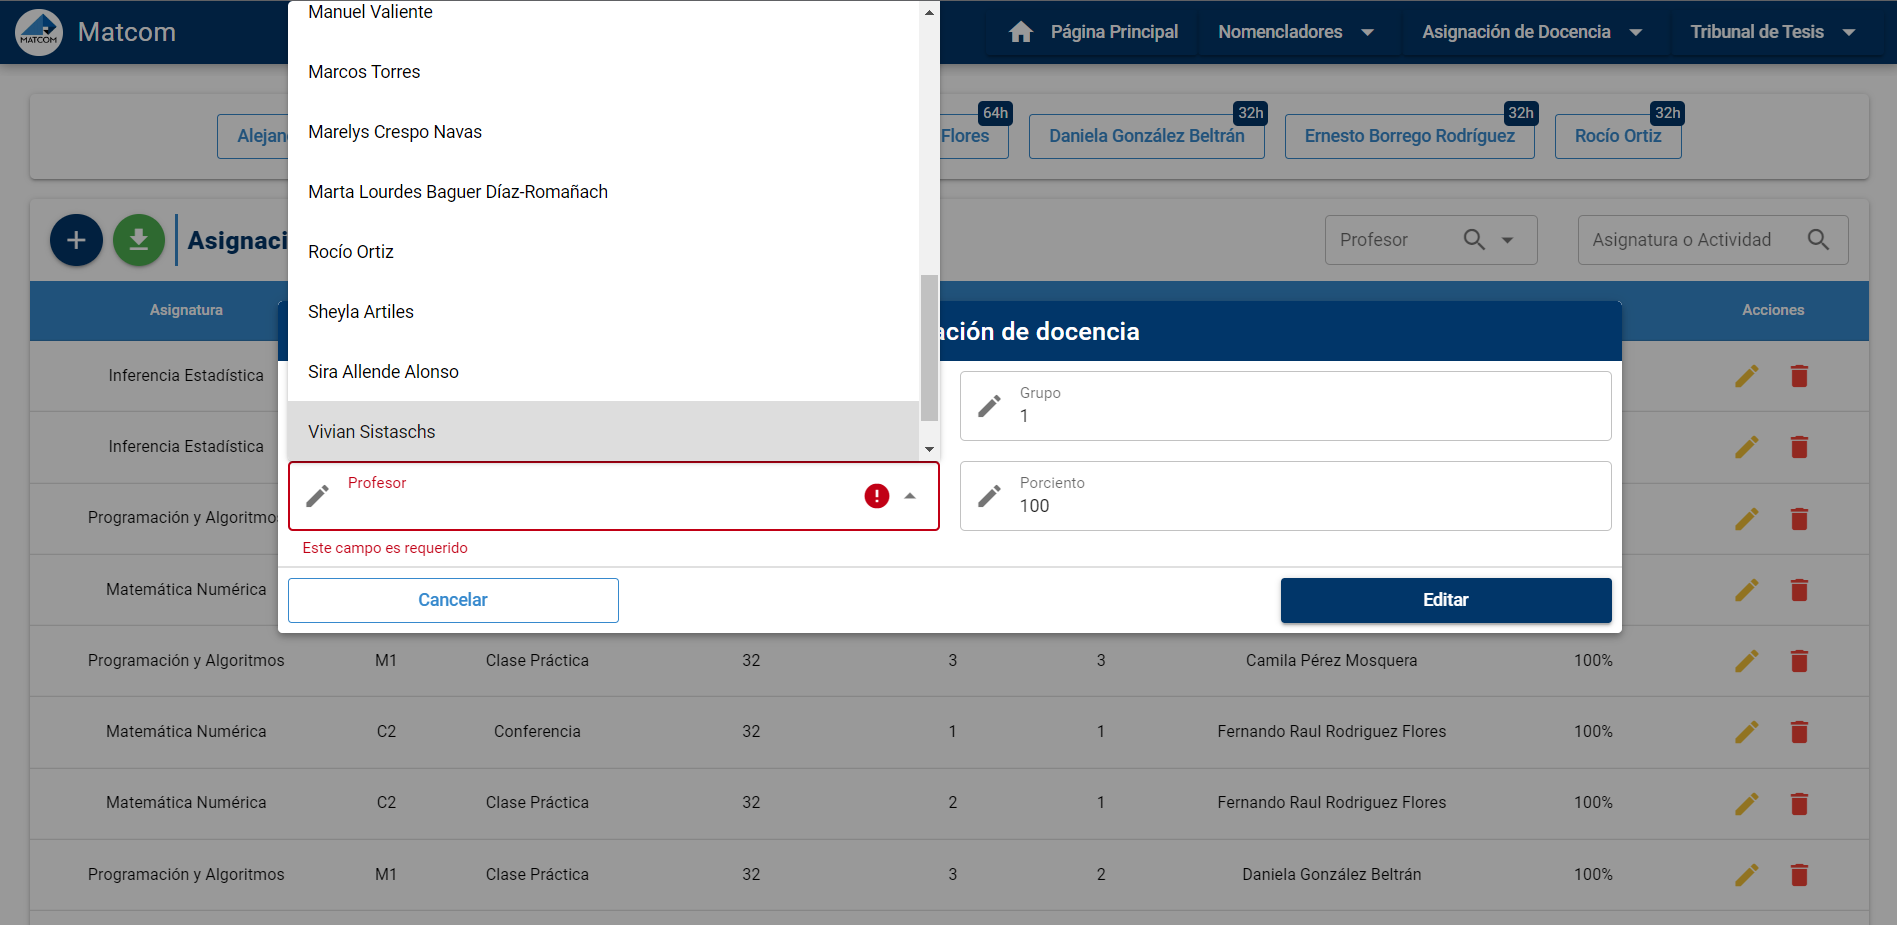
\includegraphics[scale=0.3]{Graphics/Implementation/Docencia/AD-edit-form2.png}
%     \caption{Vista del formulario para editar una asignación de docencia, mostrando los profesores posibles para la asignación}
%     \label{img-ta-edit-form2}
% \end{figure}



% La figura \ref{img-ta-result} muestra el resultado de completar los pasos
% que se muestran en la figuras \ref{img-ta-ordering}, \ref{img-ta-edit-form1} y \ref{img-ta-edit-form2}.

% % \begin{figure}[H]
% %     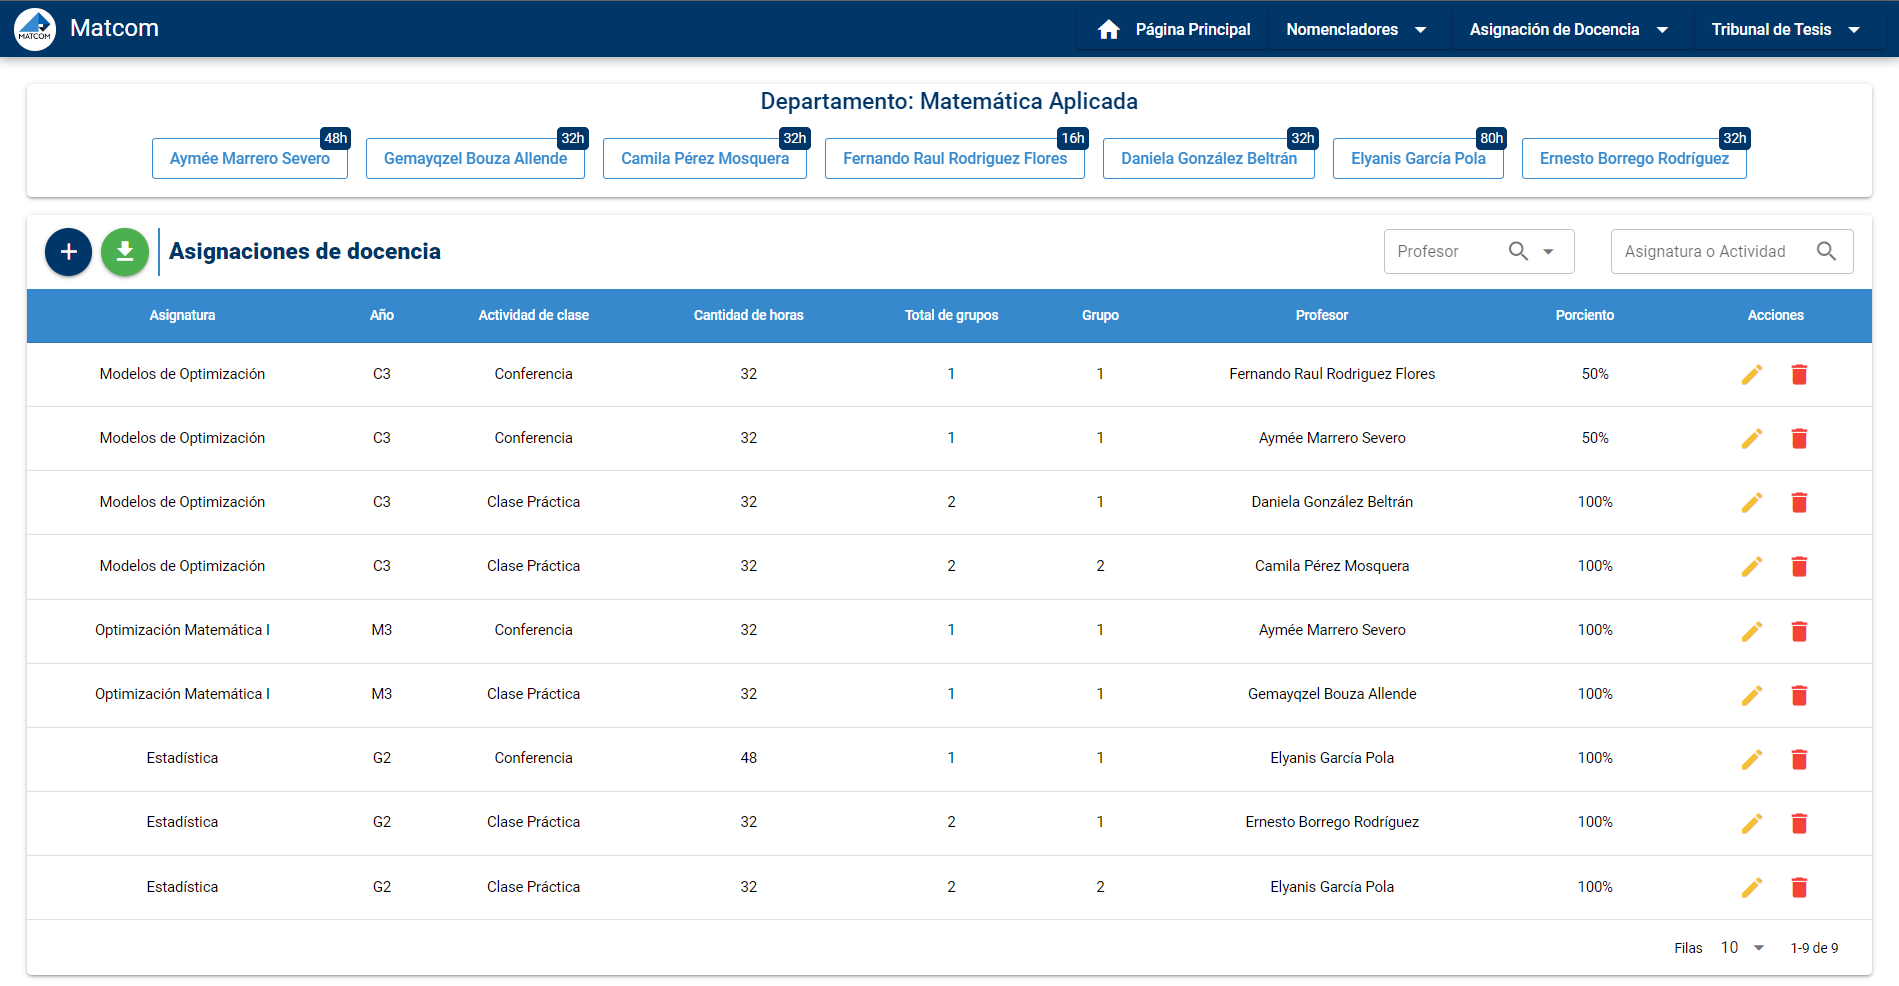
\includegraphics[scale=0.3]{Graphics/Implementation/Docencia/AD-result.png}
% %     \caption{Vista de la asignación tras realizar una asignación correctamente}
% %     \label{img-ta-result}
% % \end{figure}

% Cada vez que se realicen cambios en la tabla, ya sean por agregar, editar o eliminar 
% asignaciones de docencia, la carga docente de los profesores se actualiza como se indica 
% en el recuadro A. El recuadro B refleja como quedó la fila tras la asignación de la profesora 
% Vivian Sistaschs para que imparta las 48 horas de conferencia de la asignatura Inferencia Matemática
% a los estudiantes que cursan el tercer año de la carrera Matemática.



En la siguiente sección se describen los pasos para realizar la confección de los 
tribunales y la planificación de las defensas de tesis.

\section{Planificación de las tesis} \label{cap4:tesis}
La planificación de las tesis consta de dos subprocesos principales: la confección de los tribunales 
y la programación de las defensas. 
En esta sección se describen los pasos a seguir para completar 
la planificación de las tesis a través del sistema.
Para ilustrar este proceso se utilizará el mismo ejemplo que se 
describe en la sección \ref{tesis:cap2}. 
En la tabla \ref{tabla-tesis-cap4} se muestran los datos de dos 
tesis, en la tabla \ref{tabla-tribunal-tesis-cap2} el tribunal seleccionado y en 
la tabla \ref{tabla-defensa-tesis-cap4} el horario escogido para la defensa de las mismas.

\begin{table}[H]
    \centering
    \begin{tabular}{ | c | c | c | c |}
      \hline
      \thead{ID} & \thead{Tesis} & \thead{Estudiante} & \thead{Tutores} \\
      \hline 
             1 & \makecell{Simulación y optimización \\ de movimientos de malabares} & Gustavo Despaigne & Fernando Rodríguez  \\
      \hline
             2 & \makecell{Propagación de epidemias \\ mediante modelos basados \\ en metapoblaciones} & Abel Antonio Cruz & \makecell{Angela M. León \\ José A. Mesejo} \\
      \hline
    \end{tabular}
    \caption{Datos de las tesis}
    \label{tabla-tesis-cap4}
\end{table}


\begin{table}[H]
    \centering
    \begin{tabular}{ | c | c | c | c |}
      \hline
      \thead{ID Tesis} & \thead{Tutores} & \thead{Oponente} & \thead{Presidente} \\
      \hline 
             1 & Fernando Rodríguez & Gemayqzel Bouza & Aymeeé Marrero  \\
      \hline
             2 & \makecell{Angela M. León \\ José A. Mesejo } & Damian Valdés & Gemayqzel Bouza  \\
      \hline
    \end{tabular}
    \caption{Posibles tribunales para las tesis tesis}
    \label{tabla-tribunal-tesis-cap4}
\end{table}

\begin{table}[H]
    \centering
    \begin{tabular}{ | c | c | c | c |}
      \hline
      \thead{ID Tesis} & \thead{Fecha} & \thead{Hora} & \thead{Local} \\
      \hline 
             1 & 10/12/2022 & 2:00 PM & Aula Posgrado  \\
      \hline
             2 & 10/12/2022 & 3:30 PM & Salón del Decanato \\
      \hline
    \end{tabular}
    \caption{Posible horarios para los actos de defensa}
    \label{tabla-defensa-tesis-cap4}
\end{table}


El primer paso es ingresar las tesis en el sistema,
en la figura \ref{img-tc-thesis} se muestra la interfaz de usuario
que permite realizar esta tarea.


\begin{figure}[H]
    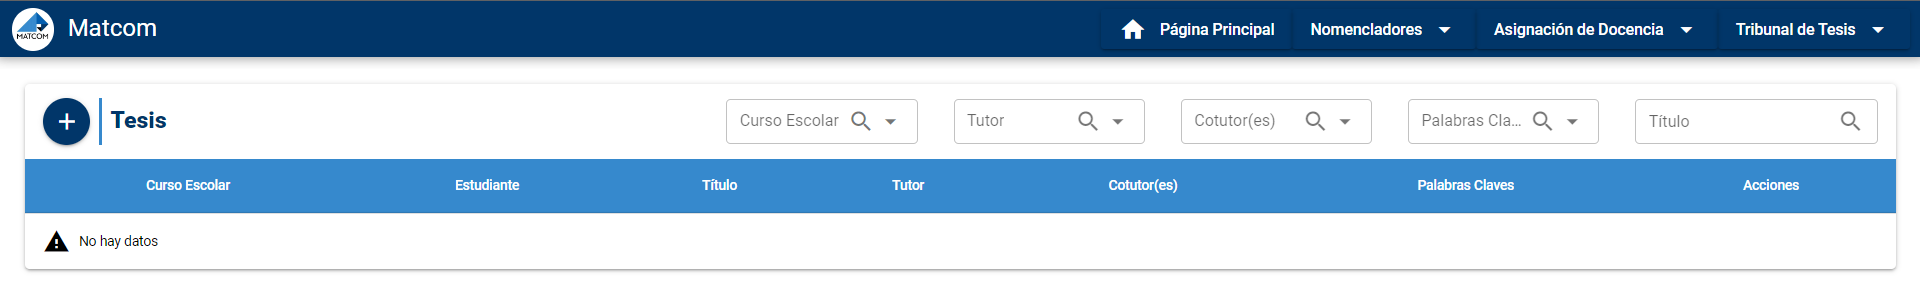
\includegraphics[scale=0.3]{Graphics/Implementation/Tesis/thesis-empty.png}
    \caption{Vista de la tesis.}
    \label{img-tc-thesis}
\end{figure}


Para agregar una nueva tesis en el sistema, se debe pulsar sobre el botón 
de agregar que se indica en el recuadro A de la figura \ref{img-tc-thesis}.
Luego se deben llenar los campos necesarios relacionados con las tesis. En la figura
\ref{img-tc-thesis-form} se muestra el resultado de pulsar sobre el botón de agregar y llenar los campos 
correspondientes a la primera tesis que se muestra en la tabla \ref{tabla-tesis-cap4}.

\begin{figure}[H]
    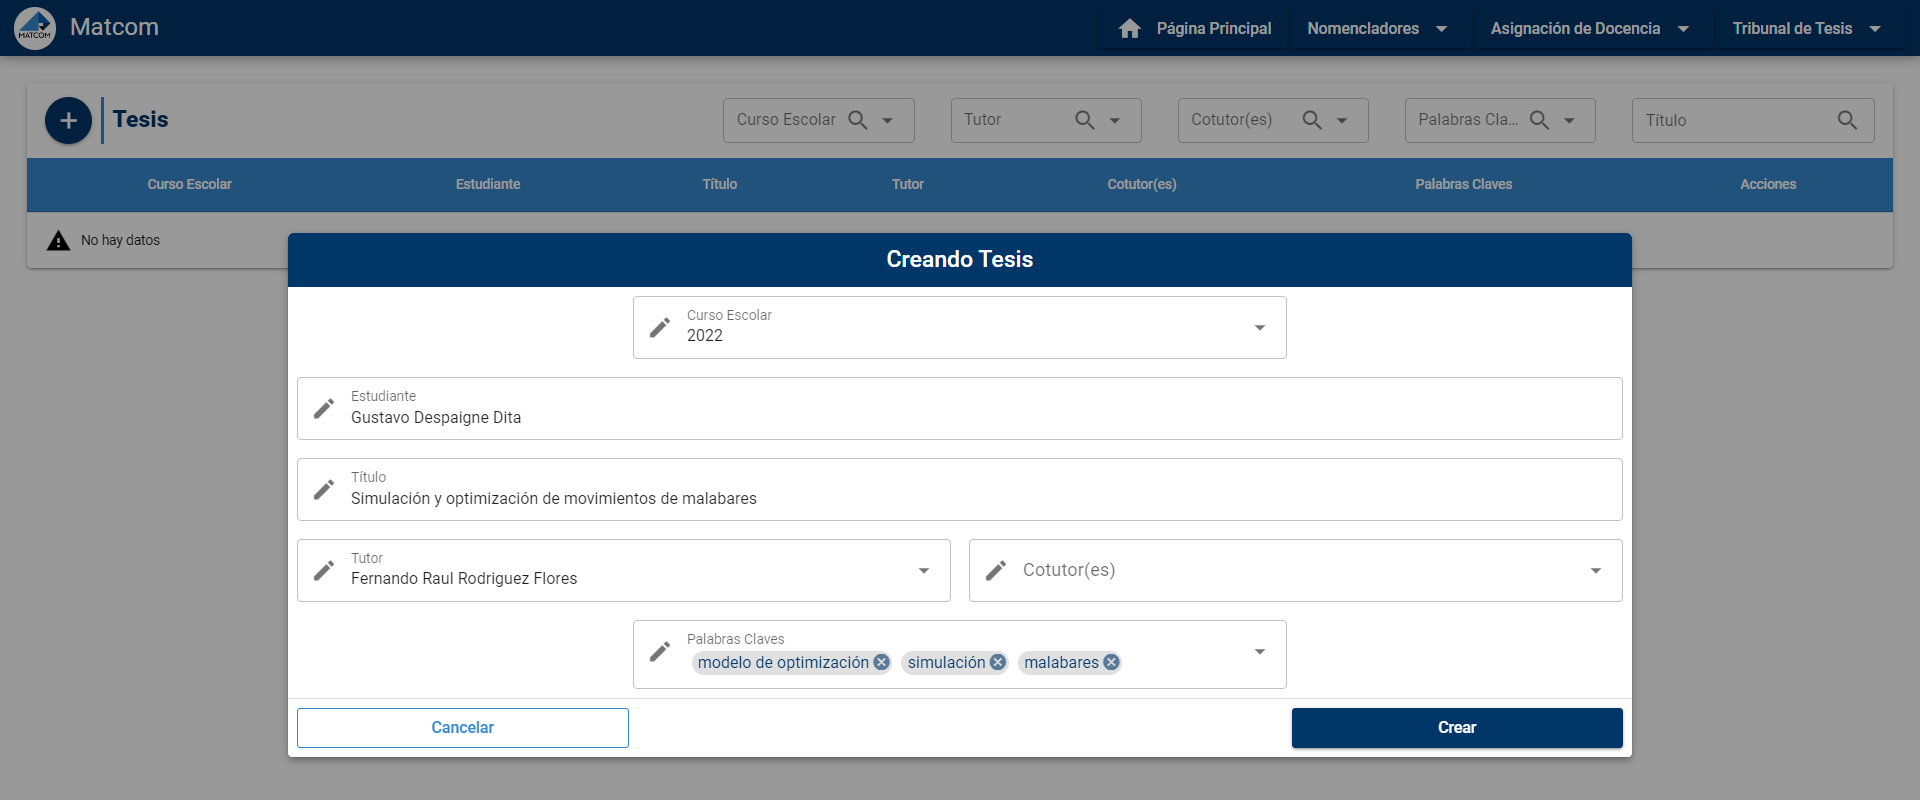
\includegraphics[scale=0.3]{Graphics/Implementation/Tesis/thesis-form.png}
    \caption{Vista del formulario para agregar una tesis.}
    \label{img-tc-thesis-form}
\end{figure}


Repitiendo el procedimiento anterior se puede agregar la segunda tesis que se 
muestra en la tabla \ref{tabla-tesis-cap4}. En la figura \ref{img-tc-thesis-result} tal
se muestra el resultado de agregar las dos tesis en el sistema.

\begin{figure}[H]
    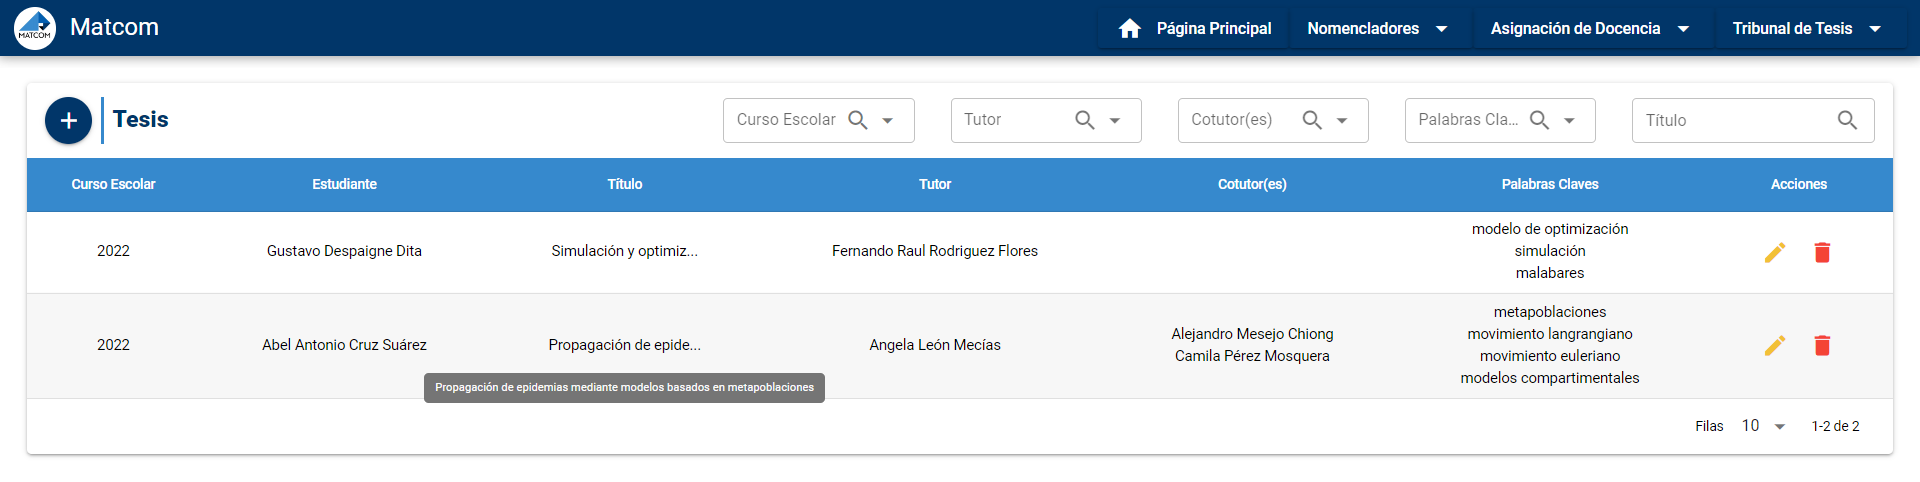
\includegraphics[scale=0.3]{Graphics/Implementation/Tesis/thesis-result.png}
    \caption{Vista de la interfaz de usuario tras agregar las dos tesis del ejemplo.}
    \label{img-tc-thesis-result}
\end{figure}

Cada vez que se agregue una tesis al sistema, se crea una  
instancia de un tribunal de tesis con los campos de oponente y presidente sin asignar.
En la figura \ref{img-tc-thesis-committee-empty}  se muestran los tribunales incompletos creados 
automáticamente a partir de las tesis que se ingresaron en el sistema.

\begin{figure}[H]
    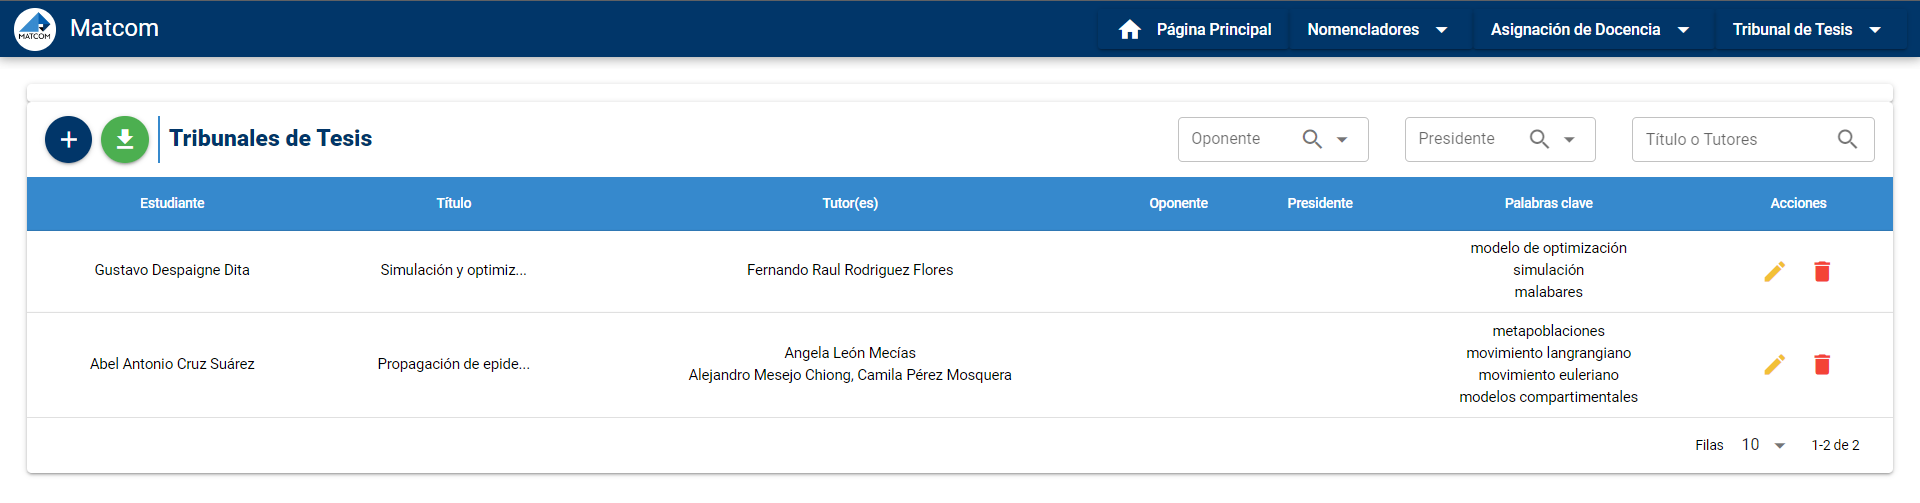
\includegraphics[scale=0.3]{Graphics/Implementation/Tesis/thesis-committee-empty.png}
    \caption{Vista de la interfaz de usuario para la confección de los tribunales.}
    \label{img-tc-thesis-committee-empty}
\end{figure}


El próximo paso es asignar los profesores que conformarán  los tribunales de tesis.
El encargado de realizar este proceso debe pulsar sobre el botón de editar 
de la fila correspondiente al tribunal que desea definir. En la figura \ref{img-tc-thesis-committee-form}
se muestra el resultado de pulsar sobre el botón de la primera fila y completar el tribunal
con los profesores que se muestran en la tabla \ref{tabla-tribunal-tesis-cap4}.


\begin{figure}[H]
    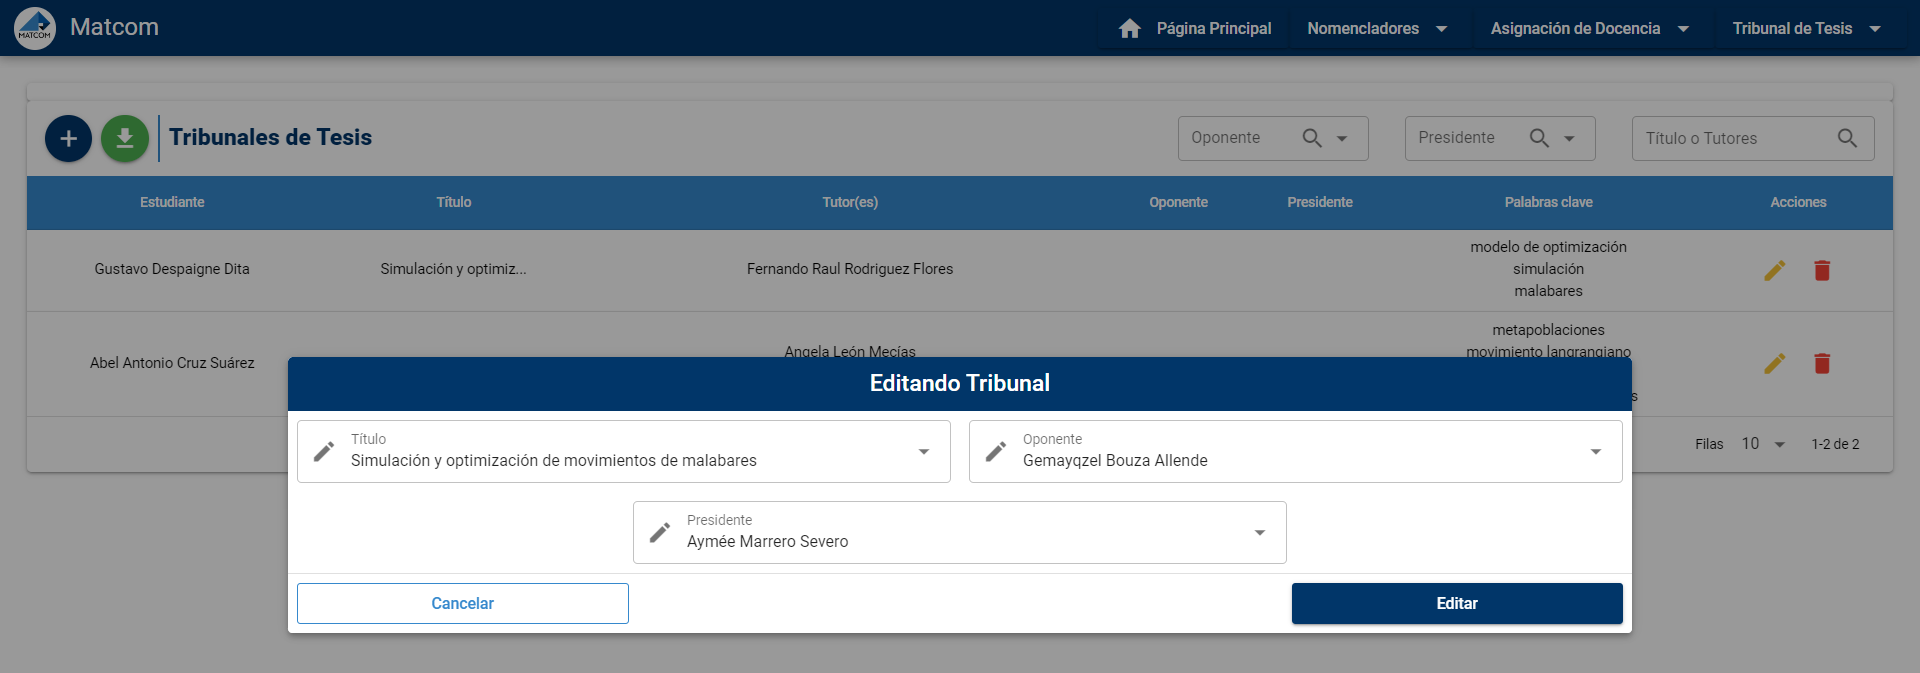
\includegraphics[scale=0.3]{Graphics/Implementation/Tesis/thesis-committee-form.png}
    \caption{Vista del formulario para la confección de los tribunales.}
    \label{img-tc-thesis-committee-form}
\end{figure}


Cada vez que un tribunal de tesis se modifique se actualiza la participación de los 
profesores en tribunales, para cada profesor se muestra la cantidad de tribunales en los que 
participa como oponente y como presidente. En la figura \ref{img-tc-thesis-committee-assign1}
se muestra el resultado de confeccionar el tribunal para la tesis del estudiante Gustavo Despaigne 
Dita.


\begin{figure}[H]
    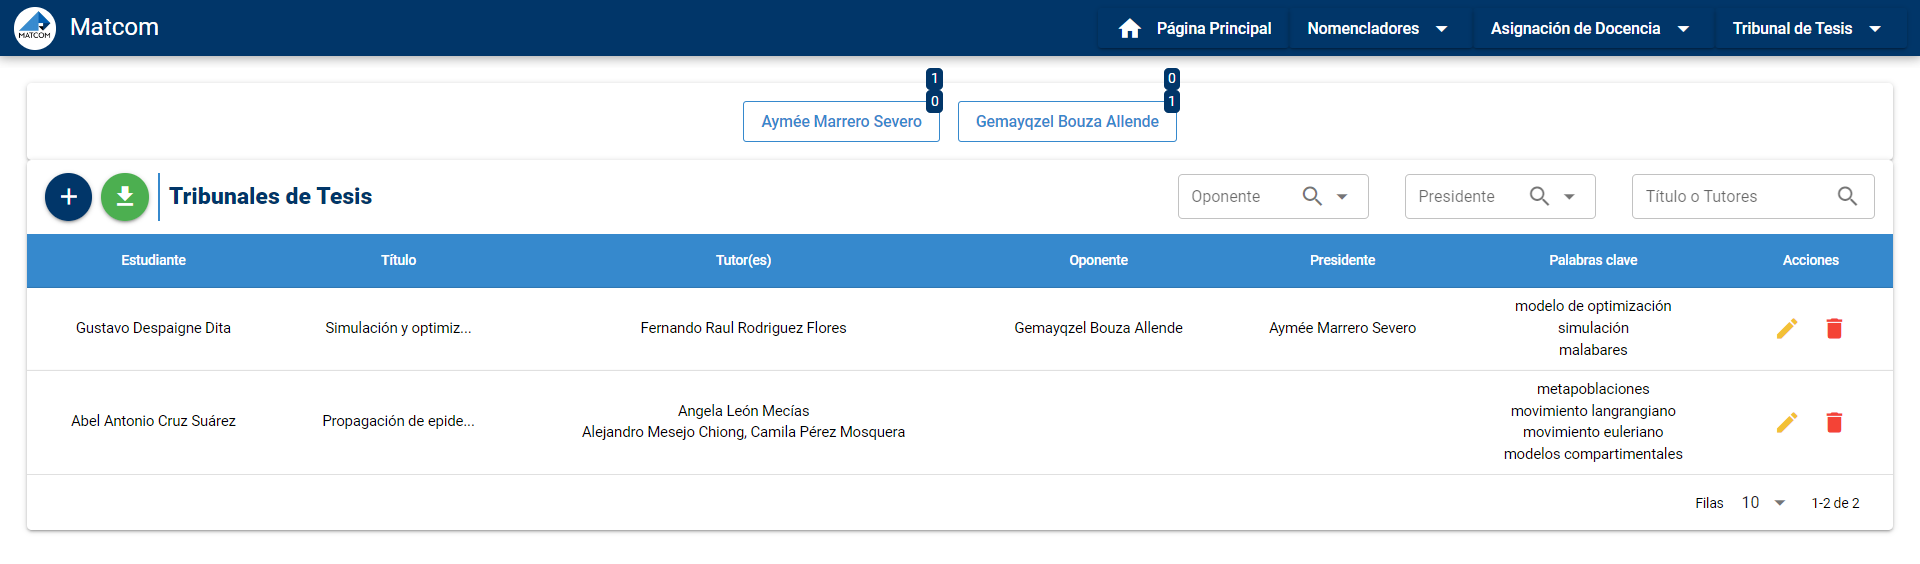
\includegraphics[scale=0.3]{Graphics/Implementation/Tesis/thesis-committee-assign1.png}
    \caption{Vista resultante de confeccionar el tribunal de la primera tesis de la tabla.}
    \label{img-tc-thesis-committee-assign1}
\end{figure}

En el recuadro A que se indica en la figura \ref{img-tc-thesis-committee-assign1},
se muestran las participaciones de los profesores en los tribunales que se hayan asignado.
En este ejemplo, la profesora Aymeeé Marrero participa en 0 tribunales como oponente y en 1 tribunal
como presidente y la profesora Gemayqzel Bouza participa en 1 tribunal como oponente y en 0 tribunales 
como presidente.
El recuadro B muestra una descripción que aparece al colocar el cursor sobre uno de los profesores, en 
este caso sobre el recuadro que representa la cantidad de tribunales en los que participa la profesora Gemayqzel.
La figura \ref{img-tc-thesis-committee-assign2} muestra el resultado de confeccionar el tribunal para la tesis del estudiante Abel
Antonio Cruz Suárez.

\begin{figure}[H]
    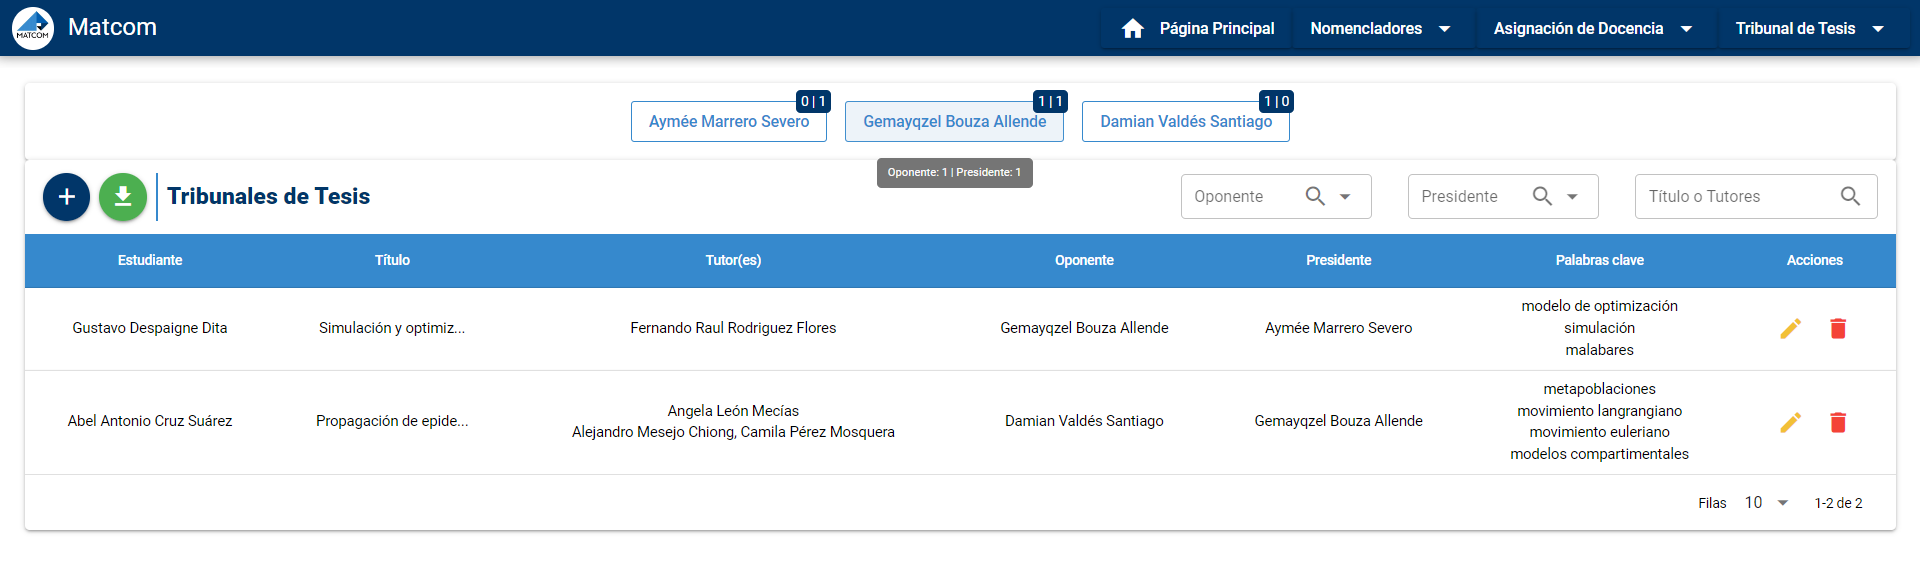
\includegraphics[scale=0.3]{Graphics/Implementation/Tesis/thesis-committee-assign2.png}
    \caption{Vista del formulario para la confección de los tribunales.}
    \label{img-tc-thesis-committee-assign2}
\end{figure}

En la figura \ref{img-tc-thesis-committee-assign2}
se puede apreciar que se actualizaron las participaciones de los profesores en los tribunales.
Se agregó la participación del profesor Damian Valdés y se actualizó la de la profesora Gemayqzel Bouza, 
aumentando en 1 la cantidad de participaciones en tribunales como presidente.


Cuando se hayan confeccionado los tribunales de tesis, el siguiente paso 
es realizar la programación de las defensas. 
Cuando una tesis se agrega al sistema, se crea una instancia 
de una defensa de tesis sin definir los campos fecha, hora y local.
En la figura \ref{img-tc-thesis-defense-empty} se muestra la interfaz de usuario donde se realiza 
el proceso de programación de las defensas.

\begin{figure}[H]
    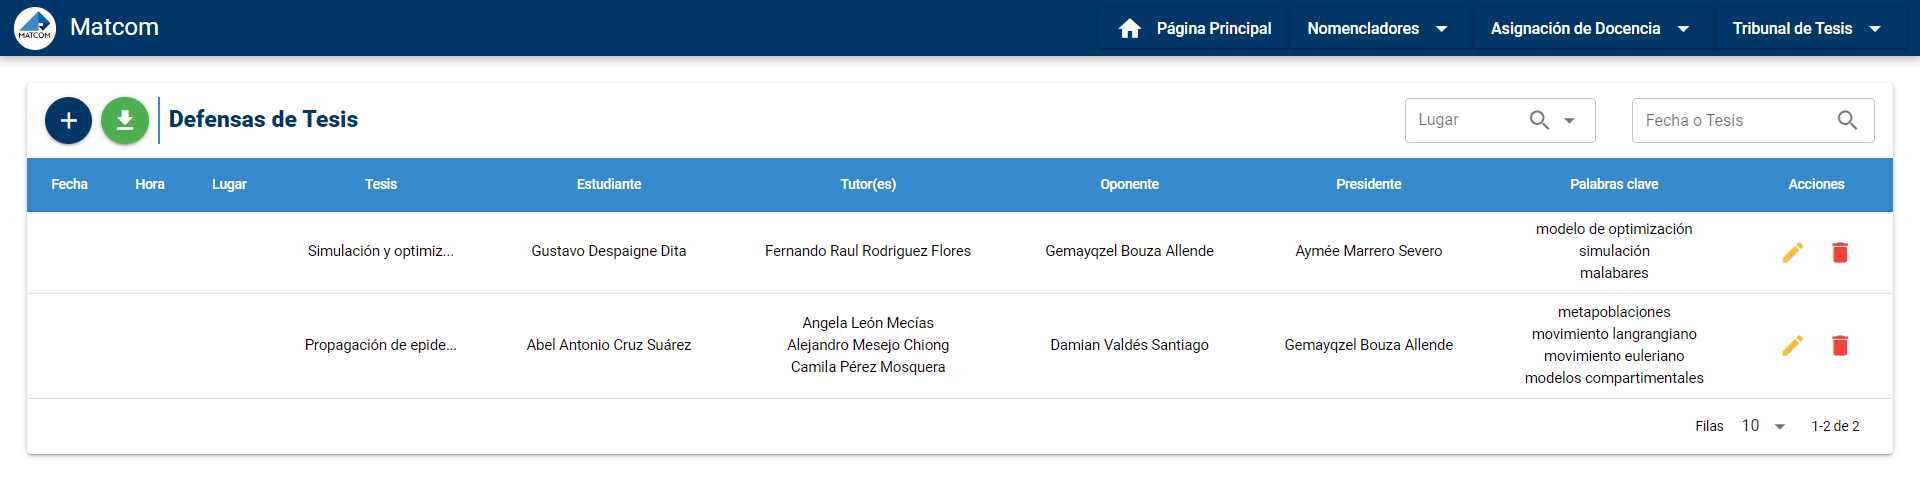
\includegraphics[scale=0.3]{Graphics/Implementation/Tesis/thesis-defense-empty.png}
    \caption{Interfaz de usario para programar las defensas de tesis}
    \label{img-tc-thesis-defense-empty}
\end{figure}

Similar al proceso de confección de los tribunales, para definir la fecha, hora y lugar 
donde se realizará la defensa de una tesis, se debe pulsar sobre el botón de editar correspondiente 
a la fila de la defensa que se desea planificar. En la figura \ref{img-tc-thesis-defense-form}
se muestra el resultado de pulsar sobre el botón de editar de la primera fila
y completar los datos de la planificación correspondiente a la tabla \ref{tabla-defensa-tesis-cap4}. 


\begin{figure}[H]
    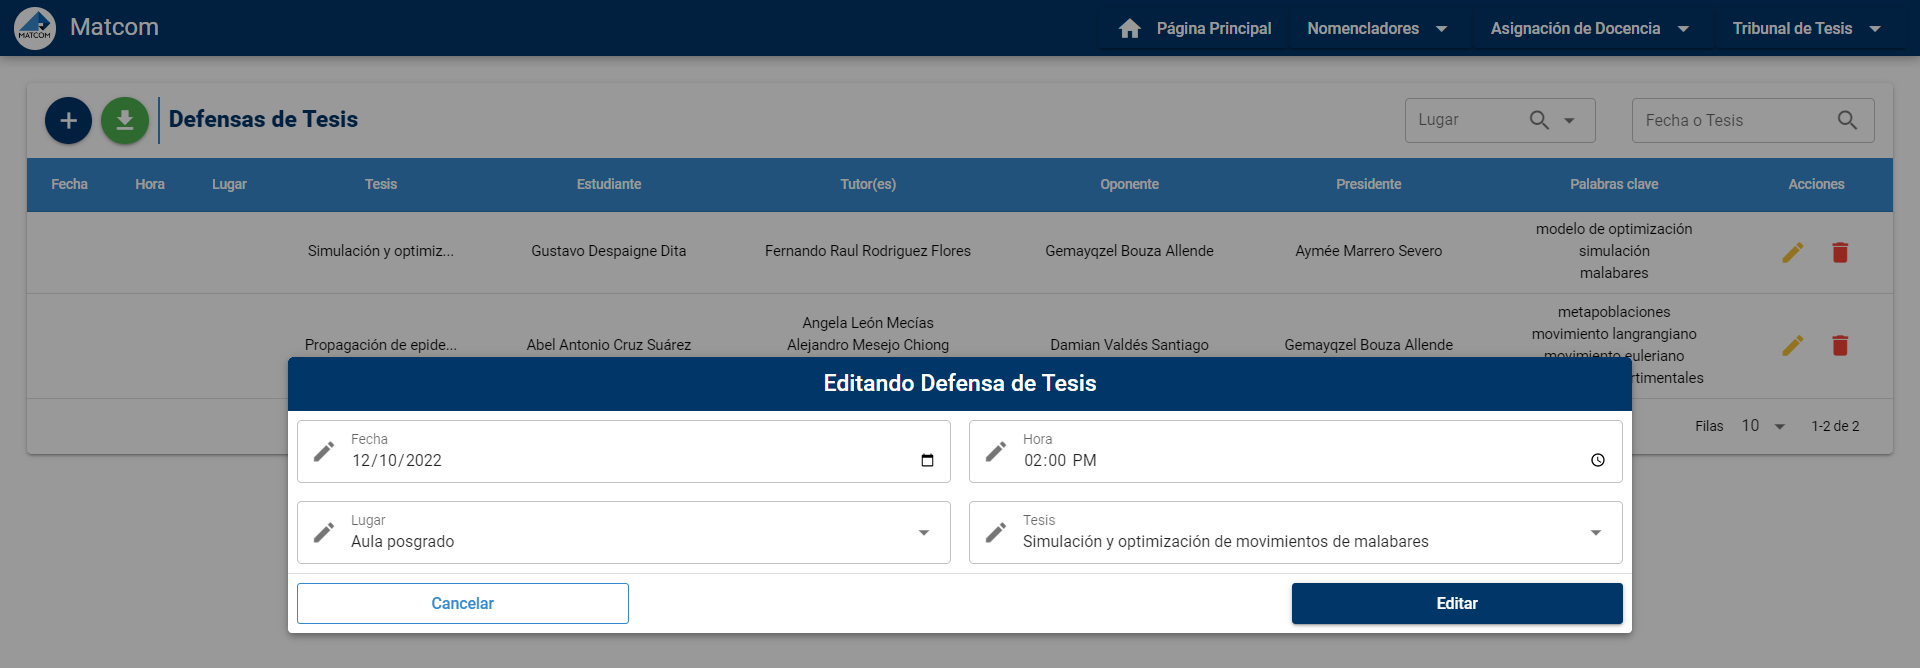
\includegraphics[scale=0.3]{Graphics/Implementation/Tesis/thesis-defense-form.png}
    \caption{Vista del formulario para la planificación de las tesis.}
    \label{img-tc-thesis-defense-form}
\end{figure}


Una vez que se hayan programado las defensas de las tesis, se puede 
exportar la información de estas a un archivo CSV pulsando sobre el recuadro A que se 
muestra en la figura \ref{img-tc-thesis-defense-result}.


\begin{figure}[H]
    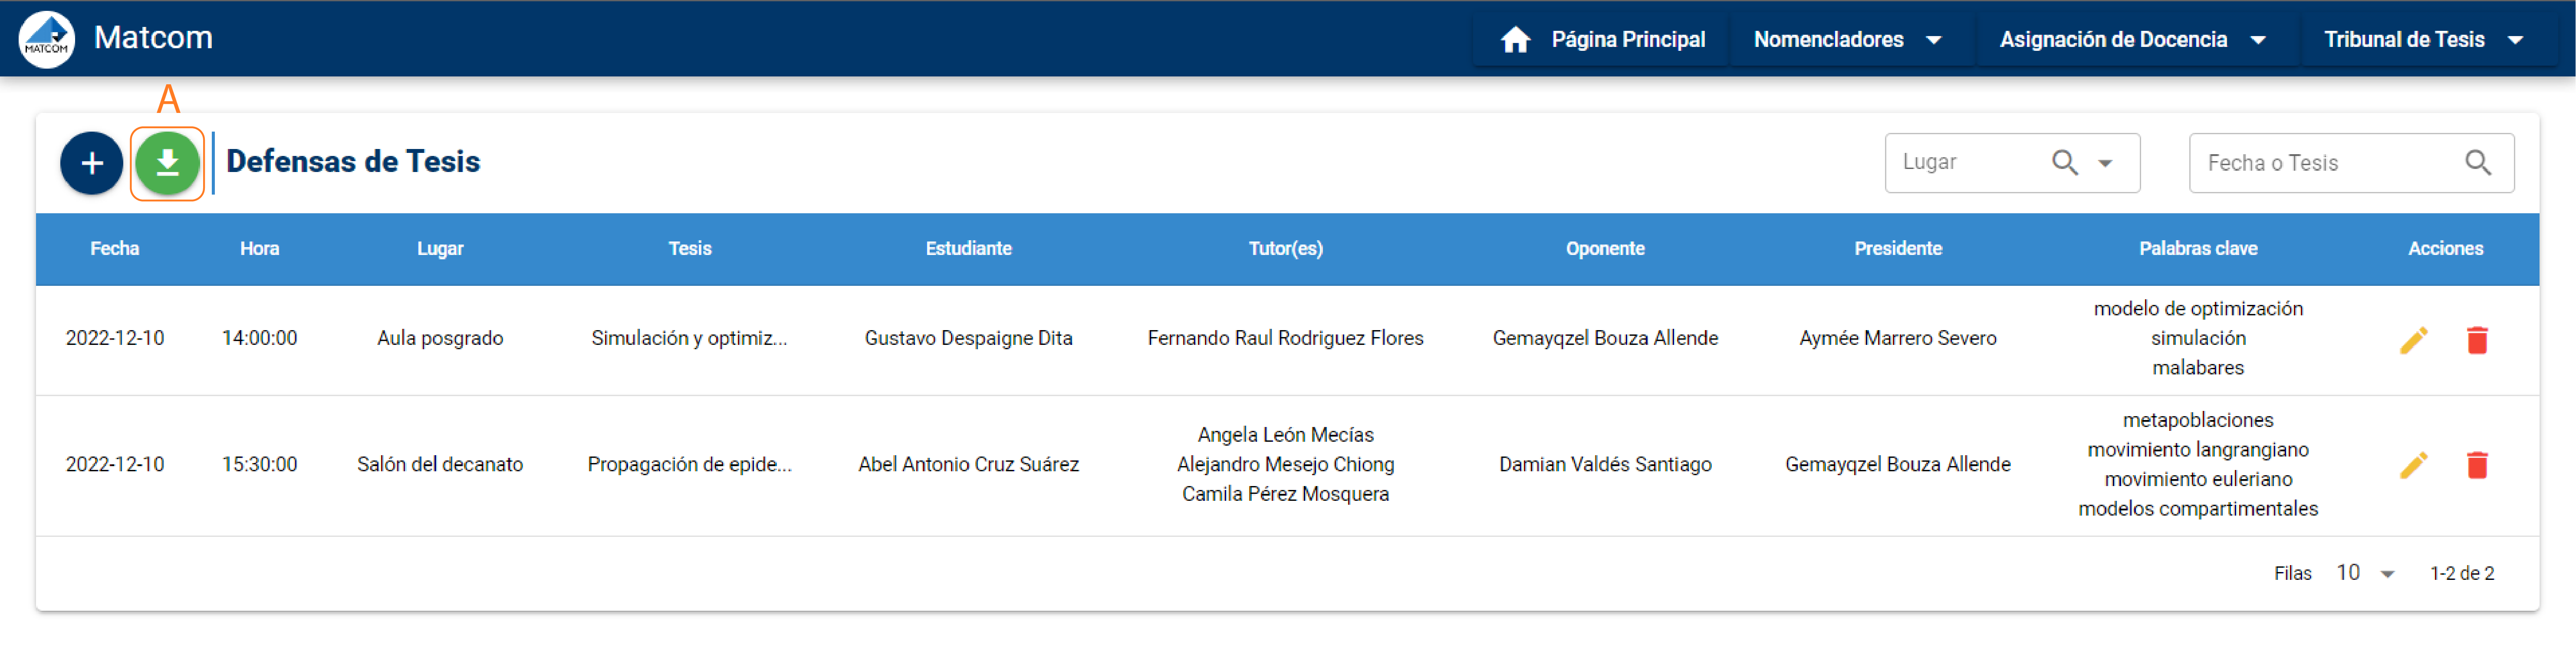
\includegraphics[scale=0.3]{Graphics/Implementation/Tesis/thesis-defense-result.png}
    \caption{Vista resultado de las planificaciones de tesis.}
    \label{img-tc-thesis-defense-result}
\end{figure}

% Para definir la fecha, hora y local donde se realizará la defensa de una tesis, se debe 
% pulsar sobre el botón de editar de la fila correspondiente a la defensa que 
% se desea planificar. En la figura tal se muestra ek resultado de pulsar sobre la fila 
% tal para planificar la defensa de la tesis tal. \\



Para poder llevar a cabo la planificación de las tesis a través
del sistema que se propone, es necesario que en la base de datos 
se ingresen las informaciones que intervienen en este proceso. Por ejemplo 
para poder confeccionar un tribunal es necesario que la tesis haya sido agregada 
anteriormente, pero para poder agregar la tesis es necesario que los tutores y 
cotutores se encuentren en el sistema. Por tanto el primer paso 
para realizar la planificación de las tesis, es ingresar todos los datos que se describen 
en la sección \ref{database:planificación-tesis}


En la siguiente sección se describen otras funcionalidades implementadas 
con el objetivo de agregar utilidad al sistema que se propone.

\section{Exportar e importar datos de la base de datos}\label{cap4:csv}

En el servidor se implementó un módulo 
que permite salvar el estado de la base de datos 
en documentos csv y poblar la base de datos a partir de los mismos.
Se crearon dos comandos para ejecutar en la terminal con el 
fin de realizar las tareas mencionadas previamente:

\subsection{Exportar los datos de la base de datos}

Se implemetó el comando \texttt{save\_database}
que permite exportar una o todas las tablas de la base de datos.
La información de cada tabla se almacena en un archivo CSV.
Para exportar la información de una única tabla
se debe especificar su nombre precedido del argumento \texttt{-m}. Por 
ejemplo para salvar la tabla que contiene la información de los profesores, se debe 
ejecutar el siguiente comando.

\begin{verbatim}
    python manage.py save_database -m Professors
\end{verbatim}


Por otra parte, si lo que se desea es exportar la información de todas las tablas 
de la base de datos a documentos CSV, se debe ejecutar el siguiente comando.

\begin{verbatim}
    python manage.py save_database
\end{verbatim}


\subsection{Importar datos a la base de datos}
Se implementó el comando \texttt{fill\_database} que permite poblar la 
base de datos a partir de los archivos CSV generados con el comando \texttt{save\_database}.
Con este comando se puede poblar una o todas las tablas de la base de 
datos. 
Para poblar la información de una única tabla
se debe especificar su nombre precedido del argumento \texttt{-m}. Por 
ejemplo para llenar la tabla que contiene la información de las asignaturas, se debe 
ejecutar el siguiente comando.

\begin{verbatim}
    python manage.py fill_database -m Subjects
\end{verbatim}

Por otra parte, si lo que se desea es importar la información de todos los archivos CSV  
para la base de datos, se debe ejecutar el siguiente comando.

\begin{verbatim}
    python manage.py fill_database
\end{verbatim}


Los posibles nombres de entidades a utilizar con
el parámetro -m tanto para el comando 
\texttt{save\_database} como \texttt{fill\_database} son:
\texttt{ClassTypes}, \texttt{Faculties},
\texttt{ScientificDegrees}, \texttt{TeachingCategories},
\texttt{Semesters}, \texttt{TeachingGroups}, \texttt{TimePeriods}, \texttt{ScholarYears},
\texttt{Careers}, \texttt{StudyPlans}, \texttt{CarmenTable}, \texttt{Departments},
\texttt{Subjects}, \texttt{Professors}, \texttt{SubjectDescriptions}, \texttt{TeachingAssignments},
\texttt{Places}, \texttt{Keywords}, \texttt{Thesis}, \texttt{ThesisCommittee}. \\


En este capítulo se describieron los pasos a seguir para realizar la asignación de docencia 
y la planificación de las tesis a través del sistema que se propone. Se ilustraron las principales 
funcionalidades que se deseaban incorporar como: conocer la carga docente de los profesores durante 
el proceso de asignación, conocer la cantidad de participaciones de los profesores en los tribunales 
y la exportación de la información de estos procesos a un documento CSV. \\

En el próximo capítulo se describe la estructura del proyecto y algunos 
detalles de implementación que pueden servir para incorporar nuevos procesos 
en el sistema de gestión implementado.

% Se implementó un modelo de optimización para la 
% generación de asignaciones de docencia, pendiente
% computar el peso de las asignaciones (dado las
% preferencias de los profesores y sus habilidades)

\chapter{Extensibilidad}\label{chapter:extensibility}
Uno de los objetivos de este trabajo es la creación de una herramienta que 
permita la posterior integración de procesos de administración y planificación 
que se llevan a cabo en la Facultad de Matemática y Computación de la Universidad
de La Habana. 
En este capítulo propone una guía de cómo agregar nuevos 
procesos al sistema de gestión que se implementó.

En la siguiente sección se describe cómo están estructurados los proyectos 
servidor y cliente. 

\section{Estructura del cliente y servidor}
El desarrollo en el lado del servidor se llevó a cabo con el  
uso de la biblioteca Django, en particular Django Rest Framework.
Para el desarrollo de los procesos de asignación de docencia y planificaciones de las 
tesis se crearon dos apps independientes de Django, con el objetivo de agrupar los ficheros 
necesarios para la modelación de cada proceso. 
En la figura \ref{img-server-structure} se muestra cómo está estructurado el servidor.




% Para la creación del proyecto se utilizó el siguiente comando.


% \begin{verbatim}
%     django-admin startproject <nombre_del_proyecto>
% \end{verbatim}

%  Para la creación de las apps de Django se 
% utilizó el comando siguiente.

% \begin{verbatim}
%     python manage.py startapp <nombre_de_la_app>
% \end{verbatim}

% Como resultado se obtuvo la siguiente estructura que se muestra 
% en la figura .

\begin{figure}[H]
    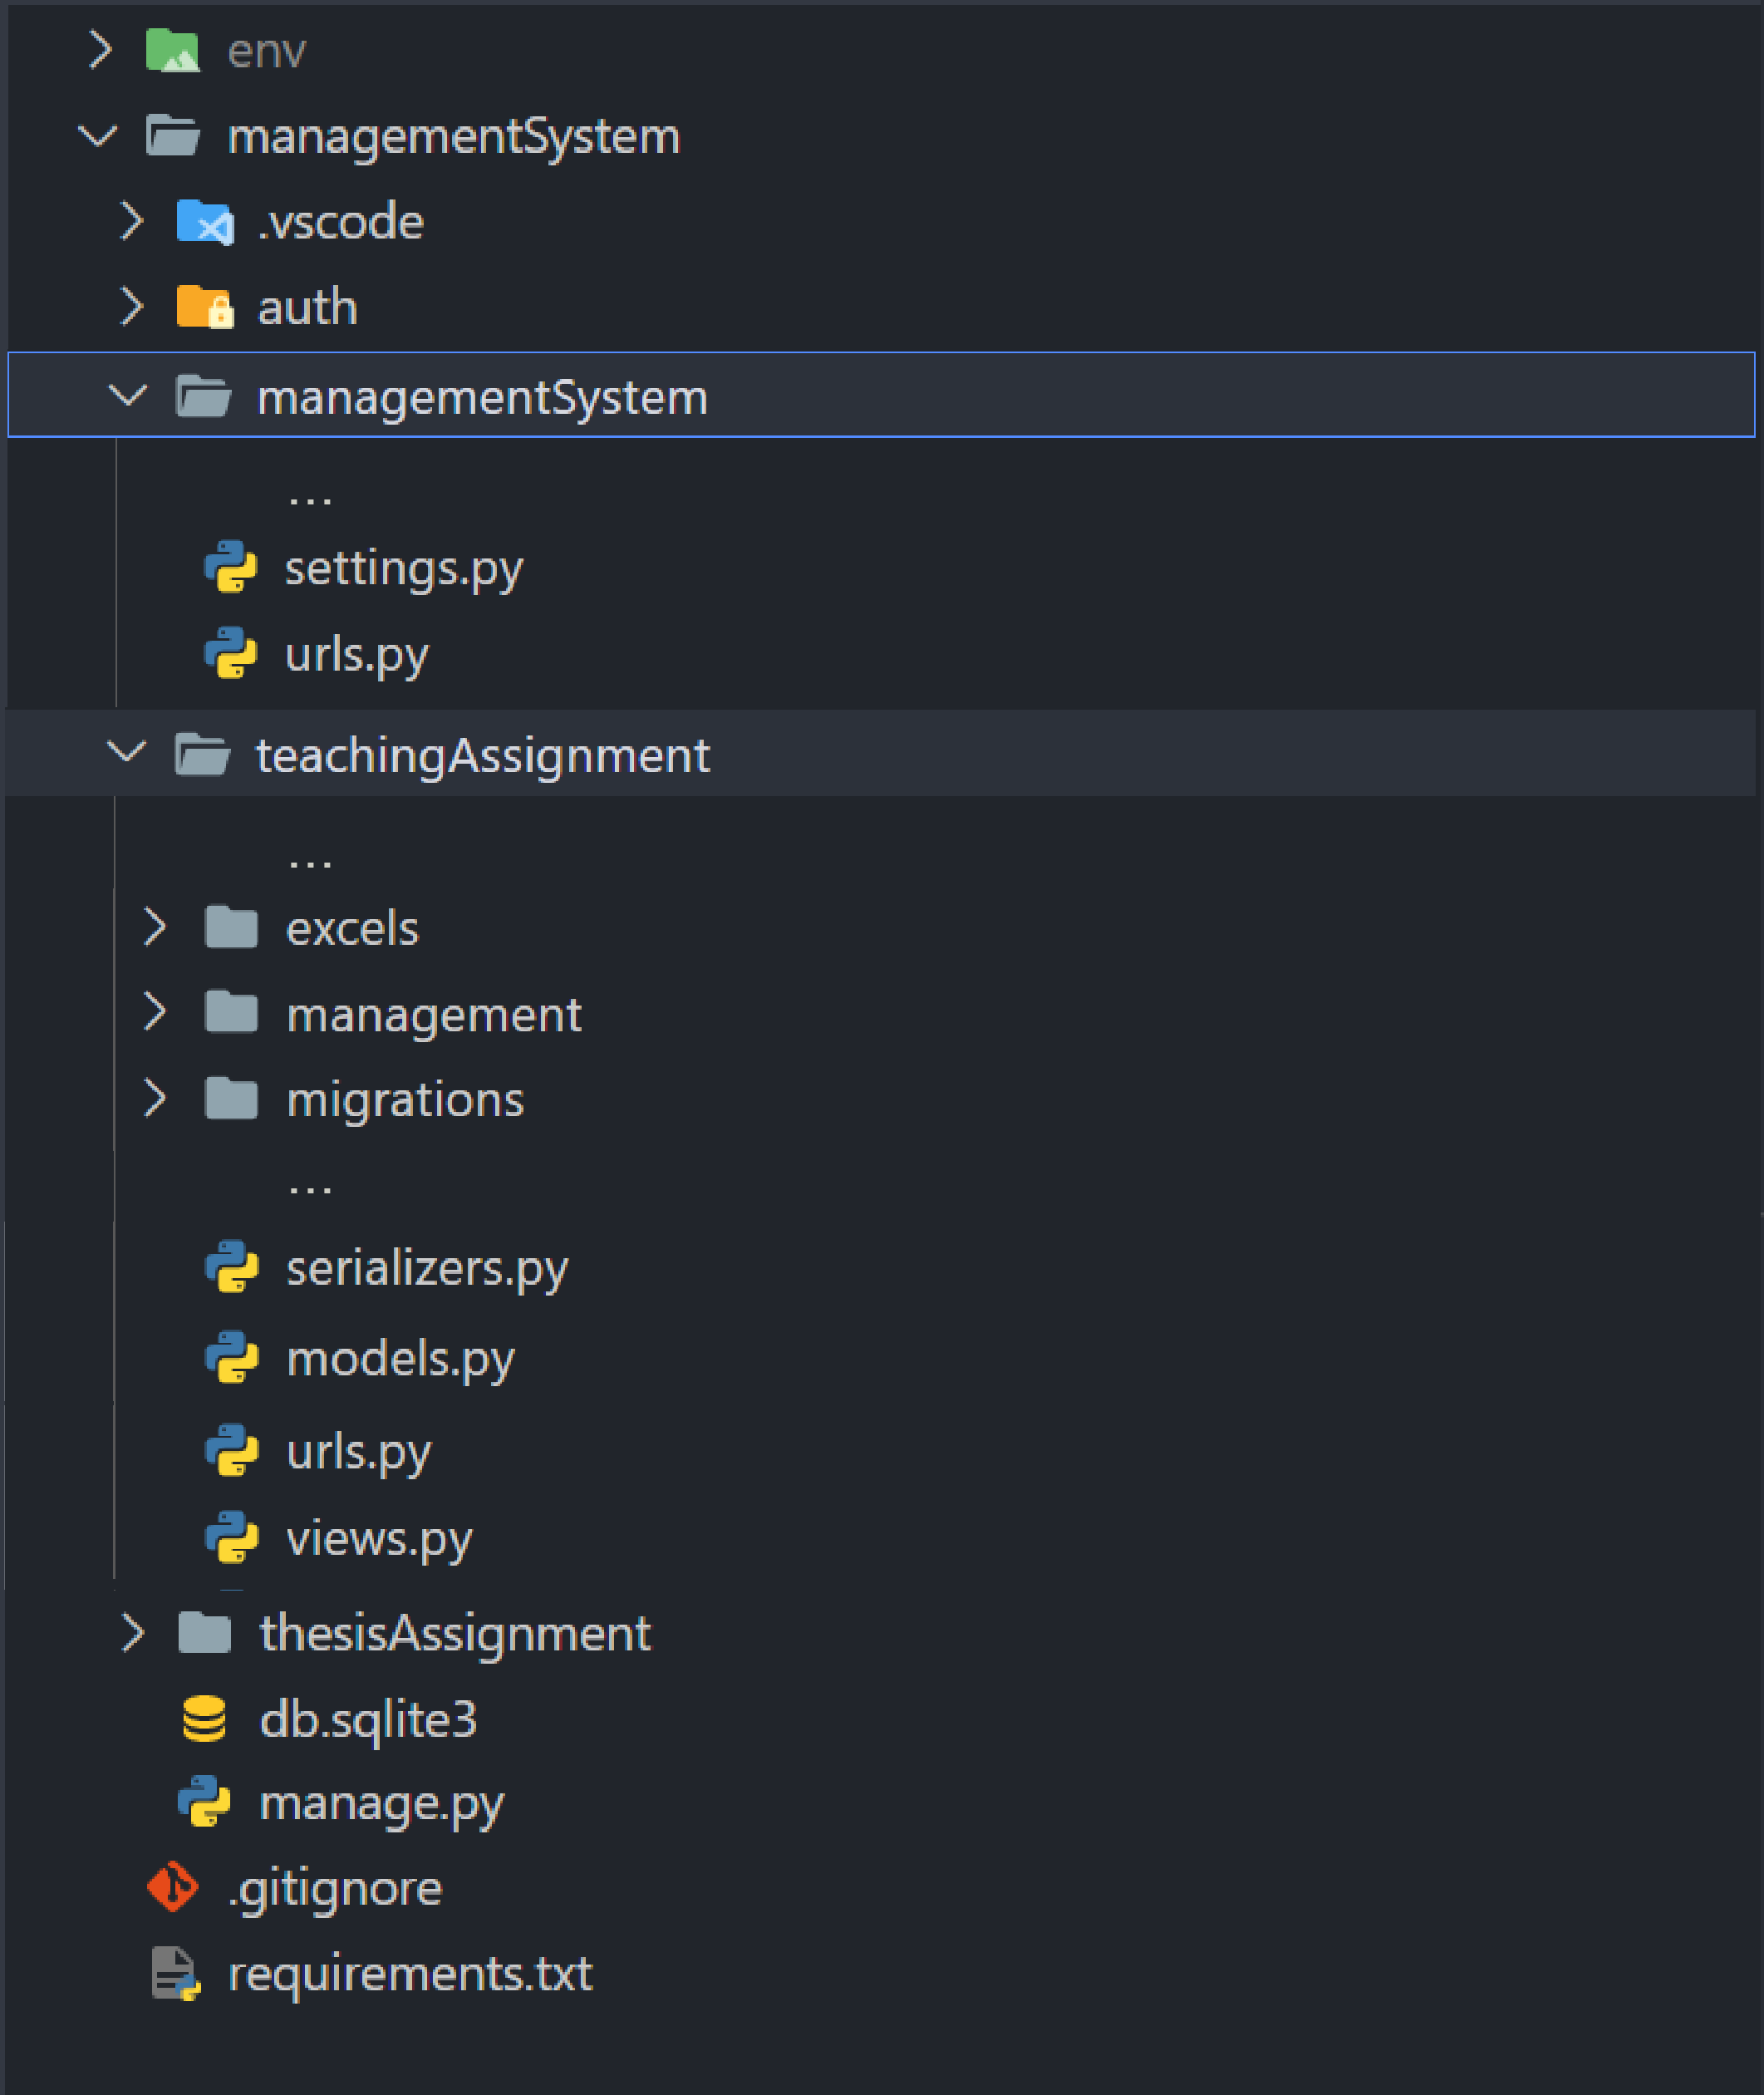
\includegraphics[scale=0.3]{Graphics/Extensibility/server-structure.png}
    \caption{Estructura de los ficheros del proyecto servidor}
    \label{img-server-structure}
\end{figure}


A continuación se describen las carpetas y ficheros principales del proyecto 
servidor.

\begin{itemize}
    \item managementSystem: es la carpeta principal del proyecto, en el fichero settings.py se encuentran
    todas las configuraciones. En el fichero url.py se deben agregar las urls de las apps creadas 
    en el proyecto. En este caso, se incluyen las urls de las apps teachingAssignment y thesisAssignment. 
    \item teachingAssignment:  app creada para el desarrollo del proceso de asignación de docencia. En la carpeta excels 
    se implementó la funcionalidad de descargar un fichero CSV con la información de la asignación de docencia. 
    \item teachingAssignment:  app creada para el desarrollo del proceso de planificación de las tesis. En la carpeta excels 
    se implementó la funcionalidad de descargar la información de los tribunales y defensas de tesis en ficheros CSV.
    \item teachingAssignment/management: en esta carpeta se encuentran las implementaciones de los comandos \textit{save\_database} 
    y \textit{fill\_database}, con los que se permite salvar y poblar la base de datos, respectivamente.
\end{itemize}


Para el desarrollo del cliente se utilizó la biblioteca Quasar. El proyecto 
cliente se inició haciendo uso de la herramienta Quasar CLI. 
La distribución de los ficheros quedó como se muestra a continuación.

\begin{figure}[H]
    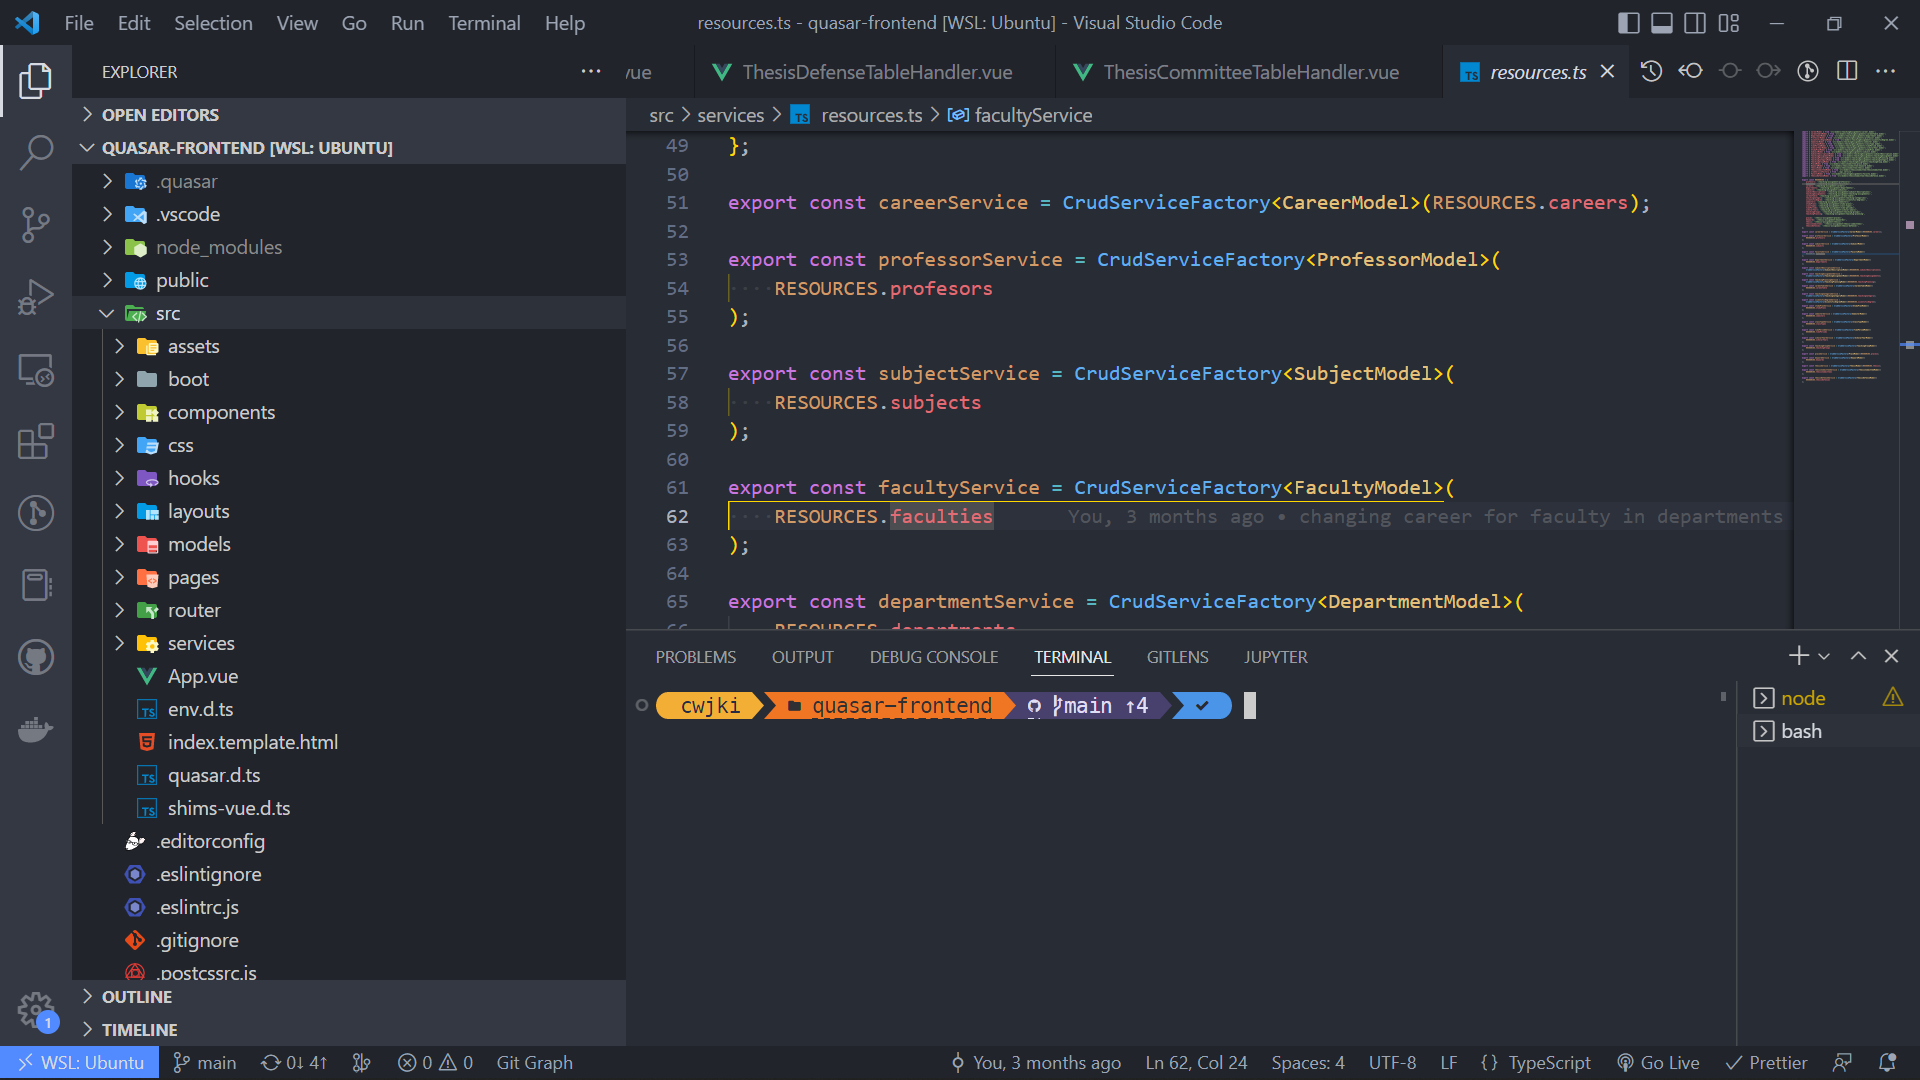
\includegraphics[scale=0.3]{Graphics/Extensibility/client-src-structure.png}
    \caption{Estructura de los ficheros del proyecto servidor}
    \label{img-client-structure}
\end{figure}

A continuación se describe qué encontrar en cada una de las carpetas principales del proyecto
cliente.

\begin{itemize}
    \item assets: las imágenes que se utilizaron en el proyecto.
    \item boot: se configura la url base para la comunicación con el servidor. 
    \item components: las componentes implementadas para el funcionamiento del proyecto. 
    Por ejemplo se creó una componente tabla para la visualización de cada una de las entidades 
    que intervienen en los procesos de asignación de docencia y planificación de las tesis. 
    \item css: los ficheros relacionados con el estilo utilizado.
    \item hooks: la implementación de un hook para conocer qué departamento se desea administrar en cada momento 
    y mostrar solo los datos relacionados con ese departamento. Por ejemplo, si se quiere realizar la asignación de docencia en el 
    departamento de Matemática Aplicada, solo se deben poder asignar los profesores que pertenezcan a ese departamento.
    \item layouts: la implementación del la barra de navegación principal.
    \item models: las definiciones de los tipos utilizados. Por ejemplo, se creó una interfaz ProfessorModel donde se definen los 
    campos que tiene un profesor, como: id, name, lastName, department, scientificDegree y teachingCategory.  
    \item pages: la implementación de las páginas de la aplicación web.
    \item router: el enrutamiento de la aplicación web.
    \item services: la implementación de una capa de abstracción para la comunicación con el servidor.
\end{itemize}


Se definió una capa de abstracción para la comunicación con 
el servidor, que permite a partir de una url, realizar las operaciones CRUD: create, read, update, delete. 
A continuación se muestra su definición.

\begin{verbatim}
    export const CrudServiceFactory = <T = any>(url: string) => {
    return {
        url: url,
        fullUrl: baseURL + url,
        create(obj: T) {
            return api.post<T>(url, obj);
        },
        list(query: Dictionary = {}) {
            return api.get<ListResult<T>>(url + buildQuery(query));
        },
        update(id: string, obj: Dictionary) {
            return api.patch<T>(url + id + '/', obj);
        },
        delete(id: string) {
            return api.delete<T>(url + id);
        },
    };
};
\end{verbatim}


En el fichero resources.ts, que se encuentra dentro de la carpeta ``services'',
se debe definir un servicio para cada uno de los endpoints 
con los que se quiera realizar la comunicación. Por ejemplo,
para realizar las peticiones relacionadas a los profesores se 
creó el servicio ``professorService'', cuyo definición se muestra a continuación.

\begin{verbatim}
    export const RESOURCES = {
        profesors: '/teaching-assignment/professors/',
        faculties: '/teaching-assignment/faculties/',
        careers: '/teaching-assignment/careers/',
        ...,

    };

    export const professorService = CrudServiceFactory<ProfessorModel>(
        RESOURCES.profesors
    );
\end{verbatim}


De esta forma, desde cualquier fichero que se importe el servicio ``professorService'',
se pueden realizar peticiones al servidor del estilo:

\begin{verbatim}
    professorService.create(obj: T)
    professorService.list(query: Dictionary)
    professorService.update(id: string, obj: Dictionary)
    professorService.delete(id)
\end{verbatim}


En la siguiente sección, se recomiendan las pautas a seguir para la incorporaración 
de nuevos procesos en el sistema de gestión.

\section{Recomendaciones para agregar un nuevo proceso en el sistema de gestión}
Para describir los pasos que se deben seguir para agregar un nuevo proceso en el sistema,
se ejemplificará con el proceso de planificación de las tesis. Supongamos que en el 
sistema de gestión solo está informatizado el proceso de asignación de docencia y se 
quiere agregar el de planificación de las tesis.

En el lado del servidor,
se recomienda crear una una app de django para encapsular los ficheros necesarios 
que intervienen en la modelación del proceso de planificación de las tesis.
Por tanto el primer paso sería ejecutar el siguiente comando.

\begin{verbatim}
    python manage.py startapp thesisAssignment
\end{verbatim}

Dentro de la carpeta thesisAssignment se deben definir los modelos, serializadores, 
vistas y urls necesarias. Para el proceso de planificación de las tesis se crearon nuevas 
entidades como Place, Keyword, Thesis, ThesisCommittee y ThesisDefense. Se modelaron sus
relaciones con otras entidades que se habían definido durante el proceso de asignación de 
docencia, por ejemplo, entre las entidadades Thesis y Professor se definieron las relaciones de tutor y cotutor.

En el lado del cliente, se siguieron los siguientes pasos para agregar el proceso 
de planificación de las tesis. 

\begin{itemize}
    \item Se creó la carpeta thesisCommittee, dentro de la carpeta src/models, para 
    agregar los tipos de las entidades que interviene en este proceso. Se agregaron las interfaces 
    KeywordModel, PlaceModel, ThesisModel, ThesisCommitteeModel y ThesisDefenseModel.
    \item En el fichero resources.ts, que se encuentra en la carpeta services, se crearon los servicios 
    placeService, keywordService, thesisService, thesisCommitteeService y thesisDefenseService, para realizar 
    las peticiones al servidor.
    \item Se creó una carpeta thesisCommittee dentro de la carpeta src/components/tables para agrupar 
    las componentes que se implementaron para la visualización de los datos en tablas. 
    \item Se creó una carpeta thesisCommittee dentro de la carpeta src/pages para agrupar 
    las vistas que necesarias para la modelación de este proceso: Keywords.vue, Place.vue, 
    Thesis.vue, ThesisCommittee.vue y ThesisDefense.vue.
    \item En el fichero routes.ts que se encuentra en la carpeta src/routes, se agregaron las rutas que llevan a las vistas definidas en el paso anterior.
    \item Se agregaron los botones que permiten ir a las vistas creadas en la barra de navegación de la aplicación web.
\end{itemize}


En resumen, en el lado del servidor, se recomienda la creación de una nueva app de Django que agrupe los ficheros necesarios para la modelación del 
proceso que se desea incorporar en el sistema de gestión. Se deben definir los modelos, cómo se serializan los datos y a través de cuáles urls se exponen.
En el lado del cliente se recomienda crear interfaces que representen el tipo de las entidades que intervienen en el proceso, definir los servicios para realizar 
las peticiones al servidor, agrupar las componentes y las vistas necesarias en carpetas que indiquen el proceso que se está informatizando y agregar un mecanismo para 
acceder a esas vistas. 

% Supongamos que se quiere agregar al sistema de gestión el proceso de planificación de 
% las evaluaciones de un semestre. A continuación se describen los pasos principales
% que se sugieren para la integración de este proceso.

% \begin{itemize}
%     \item Crear una nueva app de django con el comando tal.
%     \item Dentro de la carpeta creada en el paso anterior definir los modelos, serializadores, 
%     vistas y urls necesarios en ficheros nombrados models.py, serializers.py, views.py, urls.py respectivamente. 
%     \item Crear una carpeta con el nombre del proceso que se está modelando dentro de las carpetas pages y components. 
%     En la carpeta pages se encuentrar las vistar principales y dentro de la carpeta components definir las componentes 
%     necesarias 
%     \item En la carpeta services se implemetó una api para la comunicación con el servidor. Se creo un CRUDServiceFactory 
%     que permite realizar pedidos de crear, listar, actualizar y borrar. Solo se necesita agregar la url y el tipo de dato 
%     en el fichero resources. 
    

% \end{itemize}





\backmatter

\begin{conclusions}
    En la facultad de Matemática y Computación de la Universidad de La Habana (MATCOM)
se realizan un conjunto de procesos para administrar y planificar las actividades docentes. 
La mayoría de estas tareas se llevan a cabo de forma manual por los profesores de la facultad, lo cual representa
un derroche de tiempo que se pudiera dedicar a la investigación.
Dos de estos procesos son la asignación de docencia y la planificación de las tesis. 

En este trabajo se diseña e implementa un sistema de gestión para informatizar 
la asignación de docencia y la planificación de las tesis, creando una plataforma que permite 
la posterior integración de otros procesos.

    
Se desarrolló una aplicación web teniendo en cuenta el flujo de trabajo que se sigue actualmente para 
llevar a cabo ambos procesos, con el objetivo de facilitar la utilización del sistema como herramienta
para realizarlos.

La información necesaria para realizar la asignación de docencia y 
las planificaciones de las tesis  
se almacena en una base de datos.
Para el diseño de la base de datos se contempló la necesidad de integrar 
posteriormente la informatización y/o automatización del resto de los procesos 
administrativos de la facultad.

Además, se implementó la funcionalidad de exportar la
información correspondiente a la asignación docente,
la confección de los tribunales y la programación de las defensas de las tesis, 
con el mismo formato utilizado actualmente para la planificación de estos procesos.


Para comprobar el funcionamiento del sistema,
se reprodujo la asignación de docencia para el departamento 
de Matemática Aplicada correspondiente al período 
enero--julio del curso 2022, y se simuló la confección de los tribunales 
y la programación de las defensas de las tesis correspondientes
a este curso. 

El sistema que se propone representa una base para la informatización de la gestión de la facultad,
ya que, aunque de momento solo se informatizan la asignación de docencia
y la planificación de las tesis, se diseñó
con la perspectiva de integrar en un único sistema todas las tareas
administrativas de la facultad. \\

Algunas de las recomendaciones que se proponen son las
siguientes:
\begin{itemize}
    \item Implementar un mecanismo para automatizar la asignación de docencia.
    \item Implementar un mecanismo para automatizar la planificación de las tesis contemplando 
    las investigaciones que se han realizado en la facultad relacionadas con este tema, como 
    \cite{tribunales}.
    \item Incorporar al sistema otros procesos de gestión de la facultad.
    \item Agregar la información de la docencia externa, correspondiente a las facultades a las que se les brinda servicio.
    \item Agregar las áreas de investigación de los profesores para mejorar el proceso de confección de los tribunales.
\end{itemize}

\end{conclusions}




\begin{recomendations}
    Recomendaciones
\end{recomendations}

\printbibliography[heading=bibintoc]



\end{document}